\documentclass[12pt,a4paper,openright,twoside]{book}
\usepackage{mathtools}
\RequirePackage[utf8]{inputenc}
\RequirePackage{phd-thesis}
\addbibresource[label=biblio]{phd-thesis.bib}

\mainlinespacing{1.241} % line spacing in mainmatter, comment to default (1)

\begin{document}
	
\frontmatter
%!TeX root = phd-thesis.tex
\title{Symbolic Knowledge Injection \& Extraction for Autonomous Learning}
\author{Matteo Magnini}
\date{\today}

\newgeometry{margin=0.8in}
\begin{titlepage}
	\begin{center}
		% \vspace*{0.2cm}

		\large
		\textbf{ALMA MATER STUDIORUM -- UNIVERSITÀ DI BOLOGNA \\ DISI Dipartimento di Informatica: Scienza e Ingegneria}
		\\
		\noindent\hrulefill
		\vspace{0.4cm}

		\Large
		Doctor of Philosophy in \\
		Computer Science and Engineering

		\vspace{0.4cm}

		Cycle XXXVIII

		\vspace{0.4cm}
		%TODO: update as soon as Ilaria provides the offcial template
		Settore Scientifico Disciplinare: ING-INF/05

		Settore Concorsuale: 09/H1

		\Huge
		\vspace{3cm}
		\textbf{
			Symbolic Knowledge Injection \& Extraction for Autonomous Learning
		}

		{\Large{
		\vspace{3cm}

		\textit{Candidate:\\}
		\centering
		Matteo Magnini}
		\\}
		\large
		\vspace{2.5cm}
		\begin{minipage}[t]{0.64\textwidth}
			\begin{flushleft}
				\textit{PhD coordinator:}
				\\
				\textbf{Prof. Ilaria Bartolini}
			\end{flushleft}
		\end{minipage}
		\begin{minipage}[t]{0.34\textwidth}
			\begin{flushright}
				\textit{Supervisor:}
				\\
				\textbf{Prof.} \textbf{Andrea Omicini}
				\\
				\vspace{0.4cm}
				\textit{Co-supervisor:}
				\\
				\textbf{Prof.} \textbf{Enrico Denti}
			\end{flushright}

		\end{minipage}\\

		\vfill
		\noindent\hrulefill
		\vspace{0.3cm}
		\Large
		%TODO: update as soon as Ilaria provides the offcial template

		Esame finale anno 2025
	\end{center}
\end{titlepage}
\restoregeometry

\begin{abstract}
    %
    \Gls{AI} represents one of humanity's most transformative technological advancements, with roots in the mid‑20th century and rapidly growing societal impact.
    %
    Over the past decade, the field of \gls{NeSy} \gls{AI} -- which seeks to integrate \emph{symbolic} and \emph{sub-symbolic} approaches -- has gained increasing prominence as a promising paradigm for building intelligent systems.
    %
    By combining the structured reasoning capabilities of symbolic \gls{AI} with the adaptability and scalability of sub-symbolic methods, \gls{NeSy} \gls{AI} aims to overcome the inherent limitations of each paradigm, paving the way for more robust and interpretable systems.

    Within this broad and multifaceted landscape, this thesis focuses on two complementary subfields of \gls{NeSy} \gls{AI}: \gls{SKI} and \gls{SKE}.
    %
    These two areas, often seen as \emph{two sides of the same coin}, provide foundational mechanisms for the development of hybrid intelligent systems.
    %
    \Gls{SKI} enables the injection of structured domain knowledge into sub-symbolic models, guiding their behavior, improving generalization, and enhancing trustworthiness.
    %
    \Gls{SKE}, conversely, facilitates the extraction of symbolic, human-understandable information from these models, bridging the gap between opaque internal representations and interpretability.
    %
    Together, \gls{SKI} and \gls{SKE} form a synergistic loop: while \gls{SKI} influences learning by introducing external structure, \gls{SKE} enables inspection, verification, and refinement of that structure, contributing to the creation of systems that are explainable, reliable, and adaptable to real-world complexity.

    This thesis explores the challenges and opportunities of \gls{NeSy} \gls{AI}, with a particular focus on \gls{SKI}, \gls{SKE}, and their role in the engineering of intelligent systems.
    %
    After an overview of the background and state of the art, we identify key challenges in integrating symbolic and sub-symbolic paradigms.
    %
    We then present original contributions in the form of methodologies, algorithms, and tools designed to advance the capabilities of \gls{NeSy} systems.

    The advent of \glspl{LLM} has further transformed the landscape of \gls{AI}, offering unprecedented capabilities for understanding and generating natural language.
    %
    This thesis investigates how \glspl{LLM} can augment \gls{SKI} and \gls{SKE}, providing new avenues for designing systems that learn and adapt autonomously.
    %
    By leveraging these models, we demonstrate how hybrid approaches can address complex challenges -- such as fairness and decision-making in healthcare -- while ensuring interpretability and alignment with ethical principles.

    Finally, we discuss how these advancements align with the broader vision of \gls{NeSy}, while also contributing to the specific goal of this thesis: enabling the development of systems capable of fully autonomous learning.
    %
    These systems integrate the structured reasoning of symbolic \gls{AI}, the adaptability of sub-symbolic models, and the transformative potential of \glspl{LLM}, opening pathways toward more versatile and intelligent applications.
    %
    Such progress not only advances the field but also brings us closer to the distant horizon of general \gls{AI}, where machines can learn, reason, and adapt autonomously.

    \sloppypar
    \textbf{Keywords} -- \emph{\acrlong{AI}, \acrlong{NeSy} \gls{AI}, \acrlong{SKI}, \acrlong{SKE}, \acrlong{LLM}, intelligent systems, autonomous learning.}
\end{abstract}


\begin{dedication}
    %
    ``The work of each individual contributes to a totality, and so becomes an undying part of the totality.
    %
    That totality of human lives -- past and present and to come -- forms a tapestry that has been in existence now for many tens of thousands of years and has been growing more elaborate and, on the whole, more beautiful in all that time.
    %
    % Even the Spacers are an offshoot of the tapestry and they, too, add to the elaborateness and beauty of the pattern.
    %
    [\dots] An individual life is one thread in the tapestry and what is one thread compared to the whole?
    %
    Daneel, keep your mind fixed firmly on the tapestry and do not let the trailing off of a single thread affect you.''

    ---Isaac Asimov, \emph{Robots and Empire}
    %
\end{dedication}

\begin{acknowledgements} % this is optional
    %
    First and foremost, I would like to thank my parents, Barbara and Marcello, for their unconditional love and support throughout my life.
    %
    I thank my beloved wife, Aqila, for the never ending encouragement and for always pushing me to aim at greater goals.
    %
    I am grateful to my entire family for their help during these years.

    I want to thank my supervisor, Andrea, for his wise advice, continuous support, and for giving me the freedom to explore my ideas.
    %
    I thank my close collaborator, and de-facto a co-supervisor, Giovanni, for his invaluable insights, constructive criticism, and for always being available to discuss ideas and challenges.
    %
    I thank all the other researchers I collaborated with during these years, including Gianluca, Sara, Roberta, Andrea A., Andrea R., Federico and many others.
    %
    I also want to mention -- even if I do not explicitly list all the names -- the researchers of the Lab 4.0 for the shared experiences and the fun times we had together.
    %
    Finally, I thank Ana for being my supervisor during my visiting at the University of Oslo, and for her precious guidance and support.

    Life is also outside Academia, actually, life is mostly outside Academia.
    %
    At the very end of this journey I decided to get married, and I want to thank all my friends who made this day unforgettable and help me in the organization.
    %
    I think I almost lost my mind putting together the writing of this thesis with the wedding organization, but I made it, and I am still (probably) sane.
    %
    Aside from the wedding, these years have been full of emotions, trips, cool experiences and tough moments.
    %
    Eliciting everyone would be infeasible, but I want to mention a few of them.
    %
    Alberto, Eugenio, Marco, Enrico, Michele, the researchers at IFI (Oslo university), especially Riccardo and Paul, the students and the people who frequent the Sthop pub.

    This paragraph has been added after the reviewers' comments.
    %
    Research would not be possible without the peer review process, and it is good to acknowledge the effort of those who dedicate their time to review scientific works.
    %
    At the same time it is also good to point out when a review is done just as a formality, without real care for the work being reviewed.
    %
    I particularly thank the first reviewer for its time and for the detailed and constructive feedback, which helped me improve the quality of this thesis.
    %
    Unfortunately, I cannot say the same for the second reviewer, whose comments were very superficial and not much helpful.
    %
    To be honest, it seems a very rushed -- and out of time -- review, that me myself I would not have written even for a workshop paper.

    Last but not least, I want give a special thanks to somebody that usually does not appear in the acknowledgements of a PhD thesis.
    %
    In fact, since the very beginning of my academic career right after the Master's degree, a major event has shaken the world, and it is still going on: the invasion of Ukraine by fascist Russia.
    %
    The free people of Ukraine are fighting every day to defend not only their homeland, but also the values of freedom and democracy that we all cherish, and without which scientific research itself would not be possible as we know it.

    \vspace{1em}
    \begin{flushright}
        \emph{Slava Ukraini!}

        \emph{Heroiam slava!}
    \end{flushright}

\end{acknowledgements}

\sloppy

%----------------------------------------------------------------------------------------
\dominitoc
\tableofcontents   
\listoffigures     % (optional) comment if empty
\listoftables      % (optional) comment if empty
\lstlistoflistings % (optional) comment if empty
\printglossary[type=\acronymtype,nonumberlist]
%\printnoidxglossaries
%----------------------------------------------------------------------------------------

\mainmatter
\glsresetall

\begin{refsection}
%! Author = matteomagnini
%! Date = 05/03/25

%----------------------------------------------------------------------------------------
\chapter{Introduction}
\label{ch:introduction}
\mtcaddchapter
\minitoc
%----------------------------------------------------------------------------------------

\begin{refsection}

\section{Research background and context}
\label{sec:research-background-and-context}
%
Through the course of history, humanity has experienced several socio-technological revolutions that have changed the way we live.
%
From the first industrial revolution that initiated the automation of manual labor, to the world-wide spread of computers that started the automation of processes and decision-making \sidenote{cite/talk about expert systems(?)}, we are now witnessing the \ac{AI} revolution.
%
The advent of \ac{AI} has already successfully automated cognitive tasks \sidenote{add citation to image recognition and similar}, and it is expected to go further by reaching -- and possibly surpassing -- \emph{human-level intelligence}.
%
\Ac{AI} is not a recent invention, it has been around since the 1950s.
%
The reasons why only now (in the last decade to be more precise) \ac{AI} has become ubiquitous are the presence of crucial ingredients that were missing in the past.
%
Thanks to
%
\begin{inlinelist}
    \item the enormous amount of \emph{data},
    %
    \item the improvement of \emph{memory} and \emph{computational power} -- that still follows the Moore's law --, and
    %
    \item the affordability of huge quantity of \emph{energy},
    %
\end{inlinelist}
%
\ac{AI} finally flourished again.

The first kind of \ac{AI} that was developed is \emph{symbolic}.
%
Symbolic means that there are \emph{symbols} with specific \emph{meanings} that are manipulated by algorithms.
%
Symbolic \ac{AI} follows the \emph{deductive} process of reasoning, where the system starts from a set of axioms and applies rules.
%
These kinds of \ac{AI} programs are pretty effective in well-defined domains where there are clear rules that always hold, e.g., board games,~\ac{TSP},~\acp{BWP}, etc.
%
\emph{Sub-symbolic} \ac{AI} came after, and it is based on the \emph{inductive} process of reasoning.
%
Conversely to symbolic \ac{AI}, sub-symbolic \ac{AI} does not rely on symbols that have meanings for humans, but on \emph{patterns} that are learned from data.
%
Programs that uses sub-symbolic \ac{AI} to solve a certain task are said to perform \ac{ML}, because a model needs to first learn from examples before being able to generalize to unseen data.
%
\sidenote{consider to add a sentence or two about other different kinds of algorithms based on different learning principles like RL}
%
Sub-symbolic models like \acp{NN} can reach human or super-human performance in pre-defined tasks like image recognition, natural language processing, and many others.
%
However, to be properly effective, these models usually need a huge amount of data and hardware resources.

The natural evolution in \ac{AI} research is to use both symbolic and sub-symbolic approaches together.
%
This is the idea behind \ac{NeSy} \ac{AI}, where the deductive reasoning of symbolic \ac{AI} is combined with the inductive learning of sub-symbolic models, especially \acp{NN}.
%
This branch of \ac{AI} is still relatively young; the first works that tried to combine logic rules within a \ac{NN} date back to the 90s~\cite{DBLP:conf/aaai/TowellSN90,DBLP:journals/ai/TowellS94}.


\section{Overview and contributions}
\label{sec:overview-and-contributions}
%
Lorem Ipsum

\section{Structure of the thesis}
\label{sec:structure-of-the-thesis}
%
Lorem Ipsum

\printbibliography[title=Reference,heading=bibintoc]

\end{refsection}

%----------------------------------------------------------------------------------------
%--------------------------------------- PART I -----------------------------------------
%----------------------------------------------------------------------------------------

\part{Background}
\label{part:background}

%\begin{refsection}
%! Author = matteomagnini
%! Date = 05/03/25

%----------------------------------------------------------------------------------------
\chapter{Artificial intelligent systems}
\label{ch:intelligent-systems}

\begin{flushright}
\begin{minipage}{0.5\textwidth}
    What is \emph{intelligence}?

    What is \emph{\glsentrylong{AI}}?

    What are the characteristics of an \emph{intelligent system}?

    -- \textbf{\Cref{itm:rq0}}
\end{minipage}
\end{flushright}

\minitoc
%----------------------------------------------------------------------------------------


In this chapter, we introduce the concept of \emph{intelligence} providing one of the possible definition (\Cref{sec:what-is-intelligence}) starting from the sort of intelligence in animals and humans (\Cref{subsec:intelligence-in-nature}).
%
We then introduce intelligence in computer science with insights on reasoning, learning and agency (\Cref{subsec:intelligence-in-computer-science}).
%
Then, we focus on the core background of this thesis: \gls{AI} (\Cref{sec:ai}) by providing all the necessary notions the reader needs to understand the rest of the thesis.
%
Finally, we discuss the impact and implications of \gls{AI} in modern society (\Cref{sec:ai-and-society}).

%----------------------------------------------------------------------------------------
%-------------------------------------- Intelligence ------------------------------------
%----------------------------------------------------------------------------------------

\section{What is intelligence?}\label{sec:what-is-intelligence}

Intelligence is a concept that encompasses a wide range of abilities and characteristics of single \emph{individuals} or \emph{groups}.
%
From an \emph{evolutionary} perspective, intelligence characterises some animal species -- and organisms belonging to other biological kingdoms -- from simple forms of life.
%
In the history of our planet, carbon-based life evolved from unicellular organisms to multicellular organisms, and ultimately to complex organisms with specialized cells and tissues.
%
Some of these organisms (e.g., insects) developed skills -- such as \emph{navigation}, \emph{communication}, \emph{self-organisation}, \emph{adaptation}, and so on -- that \emph{are perceived} as intelligent abilities.
%
More evolved individuals (e.g., mammals) developed even more complex forms of intelligence, such as \emph{planning}, \emph{reasoning}, \emph{learning}, etc.


In much more recent history, the carbon-based life was not the only one to ``manifest'' intelligent behaviours.
%
With the invention of the computer, also machines can perform tasks that we consider intelligent.
%
To distinguish between the intelligence of living beings and that of machines, we refer to the former as \emph{natural intelligence} and to the latter as \emph{\gls{AI}}.


Intelligence originally emerged as a result of the evolutionary process and from the interaction of organisms with each others and their environment.
%
Later, we built machines that can perform tasks that require some sort of intelligent ability.
%
However, it is us -- as humans -- \emph{to attribute} the label of intelligent to someone or something and not to others.
%
Indeed, it is said that \emph{``intelligence is in the eye of the beholder''}.
%
In this sense, we can say that intelligence is not an absolute concept, but it should be considered under a relative perspective.


Giving a single rigorous definition of intelligence is not a trivial task.
%
Furthermore, there is not one single shape of intelligence, but it can be declined in many different ways (e.g., \emph{emotional intelligence}, \emph{social intelligence}, \emph{spatial intelligence}, etc.).
%
In this thesis we do not want to stay strictly dependant to a specific definition of intelligence, nevertheless it would be useful to provide a one.
%
We give a broad definition to help the reader to get more familiar with recurrent concepts that will appear later.
%
We choose to adopt a definition inspired by a notorious satirical essay by Cipolla~\cite{cipolla2013allegro}.
%
In \emph{``The basic laws of human stupidity''}, the author classifies \emph{individuals} into four categories based on the \emph{result} of their \emph{actions}:
%
\begin{itemize}
    \item \textbf{Stupid} $\rightarrow$ losses for others and for themselves;
    \item \textbf{Helpless} $\rightarrow$ benefits for others and losses for themselves;
    \item \textbf{Bandit} $\rightarrow$ losses for others and benefits for themselves;
    \item \textbf{Intelligent} $\rightarrow$ benefits for others and for themselves.
\end{itemize}
%
Now, what is a \emph{loss} or a \emph{benefit}?
%
We can see losses and benefits as the failure or success in -- fully or partially -- achieving a certain \emph{goal}.
%
With this respect we can state that:
%
\begin{definition}[Intelligence]
    \label{def:intelligence}
    an individual (or a group) has an intelligent behaviour if it is able to \textbf{perform actions} that lead to the \textbf{achievement} of a given \textbf{goal}.
\end{definition}
%
\Cref{def:intelligence} intentionally adopts a broad notion of intelligent behaviour.
%
Under this formulation, the ability to select actions that achieve a goal may also characterize simple reactive or feedback-based systems, as well as biological processes such as homeostasis.
%
For this reason, the definition should not be interpreted as a comprehensive or exclusive account of intelligence.
%
Rather, it serves as an operational definition, sufficient to delimit the class of systems considered in this work, namely artificial agents whose behaviour is guided by internal representations and decision mechanisms.


\Cref{def:intelligence} is also similar to the definitions of intelligence collected in the work of Legg and Hutter~\cite{DBLP:journals/mima/LeggH07}, such as the definition \emph{``The capacity to learn or to profit by experience''}~\cite{sternberg2000handbook}.
%
Broadly speaking, a common feature of these definitions is that intelligence is seen as a property of an individual \emph{interacting} with an external \emph{environment}, problem, or situation.
%
This interaction is fundamental to practically all proposed definitions of intelligence.
%
Another shared characteristic is the relationship between intelligence and the ability to succeed or \emph{profit} in achieving \emph{objectives}.
%
The notion of success or profit implies the existence of a specific \emph{goal}, although the exact nature of the goal may vary across individuals or contexts.
%
What matters is the capacity of the individual to carefully select actions that lead to the accomplishment of these goals.
%
The greater this capacity to succeed across a variety of goals, the greater the individual's intelligence.
%
This perspective aligns with the idea that intelligence is not a fixed attribute but rather a dynamic ability to adapt and perform effectively in diverse scenarios.


\subsection{Natural intelligence}\label{subsec:intelligence-in-nature}

In order to survive in their environment, animals -- but also other organisms of different kingdoms such as plants or fungi -- have developed a set of abilities and some of them are perceived as intelligent.
%
For the sake of simplicity, we will consider just to animals, but many of the concepts we will talk about can be extended to other organisms.
%
Animals have a \emph{body}, and they are \emph{situated} in the physical world.
%
Through sensory organs, they can \emph{perceive} the environment and with muscles they can \emph{interact} with it.
%
They are \emph{autonomous} individuals, i.e., they are able to perform actions without the need of an external controller.


All animals are able to keep themselves alive (\emph{self-sufficiency}) until natural death or an accident occurs.
%
In addition to self-sufficiency, animals contribute to the survival of their species generating offspring.
%
To do so, they need to navigate the environment, find food, avoid predators, reproduce, and so on.


Humans have developed two main characteristics about intelligence that are no match for any other animals: \emph{reasoning} and \emph{learning}.
%
\paragraph{Reasoning}
%
Logical reasoning, or simply reasoning, is a process of drawing conclusions from premises.
%
There exists three main ways of reasoning:
%
\begin{itemize}
    %
    \item \textbf{Deductive reasoning} $\rightarrow$ it is a top-down approach that starts from a general statement and derives specific conclusions.
    %
    For example, if we know that \emph{all humans are mortal} and \emph{Socrates is a human}, we can conclude that \emph{Socrates is mortal}.
    %
    Deductive reasoning can be compared to what Kahneman calls \emph{System 2} in his book \emph{Thinking, Fast and Slow}~\cite{kahneman2011thinking}.
    %
    Kahneman describes the second system as \emph{slow thinking}, which is deliberate, effortful, logical and more rational.
    %
    \item \textbf{Inductive reasoning} $\rightarrow$ it is a bottom-up approach that starts from specific observations and derives general conclusions.
    %
    For example, if we observe that \emph{the sun rises every day}, we can conclude that \emph{the sun will rise tomorrow}.
    %
    Inductive reasoning can be mapped in the \emph{System 1} -- i.e., \emph{fast thinking} -- of Kahneman, which is automatic, effortless, intuitive and emotional.
    %
    However, this mapping should be interpreted as partial: while some forms of inductive reasoning may rely on rapid, intuitive mechanisms, \emph{System 1} also includes innate or pre-attentive processes that are not the result of learning, and more complex inductive inferences may involve deliberative components typically associated with \emph{System 2}.
    %
    \item \textbf{Abductive reasoning} $\rightarrow$ it is a form of reasoning that starts from an observation and seeks the simplest and most likely explanation (i.e., \emph{Occam's razor}).
    %
    For example, if we observe that \emph{the grass is wet}, we can conclude that \emph{it rained last night}.
    %
    This kind of reasoning is the same that is adopted by detectives to solve crimes.
    %
    Abduction also requires the use of statistics and probabilities, and therefore it deals with uncertainty (\emph{``Once you eliminate the impossible, whatever remains, no matter how improbable, must be the truth''---Arthur Conan Doyle}\footnote{a person must be aware of all the possibilities in order to not fall into a deductive error.}).
\end{itemize}


\paragraph{Learning}
%
Human beings can perform a vast array of tasks, and their ability to learn new ones is a cornerstone of their intelligence.
%
Learning is a process that allows individuals to \emph{model reality}, adapt to their environment, and share knowledge with others.
%
Broadly speaking, humans acquire new skills and knowledge in two primary ways: by generalising experience -- e.g., via \emph{inductive} reasoning --, or by \emph{deductively} inferring new knowledge from what they already hold or can obtain from others---e.g., through direct communication (talking) or indirect communication (reading)~\cite{human-reasoning-1994}.
%
In the former case, novel knowledge is formed in the learner's mind by interacting with the environment and interpreting sensory input.
%
In the latter case, knowledge is represented symbolically (e.g., through words, gestures, or diagrams), enabling communication and the transfer of meaning between individuals.
%
This symbolic representation is crucial for sharing complex ideas and building upon the collective knowledge of a society.

Animals, too, exhibit learning abilities, though the mechanisms and extent vary widely across species.
%
For instance, many animals rely on experience to adapt to their environment, such as learning to navigate, find food, or avoid predators.
%
Some species, like primates and certain birds, demonstrate the ability to use symbols or tools, which suggests a rudimentary form of modeling reality and reasoning about their surroundings~\cite{shettleworth2010cognition}.
%
In both humans and animals, learning is deeply tied to the interaction with the environment, where experiences shape the internal models of reality that guide future actions.

In humans, the ability to reason about acquired knowledge is particularly advanced.
%
This reasoning allows individuals to not only apply learned concepts but also to refine and expand them, often by integrating new information with existing symbolic representations.
%
Such reasoning processes are essential for problem-solving, planning, and innovation, which are hallmarks of human intelligence~\cite{DBLP:journals/mima/LeggH07}.
%
Moreover, the ability to share knowledge through symbolic means, such as language, has enabled humans to build complex societies and advance technologically.


\subsection{Intelligence in computer science}
\label{subsec:intelligence-in-computer-science}
%
Since the automation of computation with the invention of the computer, intelligence has always been a central topic in computer science.
%
Officially, the field of \gls{AI} was born in 1956 at the Dartmouth Conference, where a group of researchers gathered to discuss the possibility of \emph{computing towards intelligence}.
%
In this section, we provide a high-level introduction of how machines can mimic the processes of reasoning and learning that we find in natural intelligence.
%
Later, in \Cref{sec:ai} we give a detailed background on \gls{AI}.


\subsubsection{Reasoning}\label{subsubsec:reasoning-cs}
%
Every form of reasoning presupposes a structured connection between \emph{reality} and its \emph{representation}.
%
In symbolic approaches to \gls{KR}, this connection is mediated through \emph{symbols}, where the interplay between \emph{signifier} and \emph{signified} enables the encoding of meaning.
%
Symbols thus act as the bridge between the external world and computational processes, allowing reasoning systems to manipulate abstract entities while still preserving a link to the underlying semantics of the domain.
%
In this sense, reasoning is not only the mechanical application of rules, but also the interpretative activity that derives new knowledge by operating on representations whose significance is grounded in the symbolic layer of \gls{KR}.


Symbolic \gls{KR} has always been regarded as a key issue since the early days of \gls{AI}, under the assumption that intelligent behavior requires explicit forms of knowledge and mechanisms to represent and manipulate it~\cite{DBLP:journals/cacm/NewellS76,BRACHMAN2004327}.
%
When compared to arrays of numbers, symbolic \gls{KR} is far more flexible and expressive, and, in particular, more intelligible---both machine- and human-interpretable.
%
Historically, most \gls{KR} formalisms and technologies have been designed on top of \emph{computational logic}~\cite{lloyd1990computational}, that is, the exploitation of formal logic in computer science.
%
Consider, for instance, \emph{deductive databases}~\cite{green1968}, \emph{description logics}~\cite{DBLP:conf/dlog/2003handbook}, \emph{ontologies}~\cite{cimiano2006-ontologies}, \emph{Horn} logic~\cite{Mcnulty1977}, \emph{higher-order} logic~\cite{VanBenthem2001}.


Reasoning in computer science involves the process of deriving conclusions from a set of premises or facts, often encoded in a formal language.
%
Logic reasoners, such as Prolog-based systems like tuProlog~\cite{DBLP:conf/padl/DentiOR01}, play a central role in automating this process.
%
These reasoners typically follow a sequence of steps:
%
\begin{itemize}
    \item \textbf{Parsing}, the reasoner first parses the input knowledge base, which consists of facts, rules, and queries, into an internal representation;
    %
    \item \textbf{Inference}, using inference rules, such as \emph{modus ponens}~\cite{DBLP:books/daglib/0076838}, the reasoner derives new facts or verifies the truth of a query.
    %
    \item \textbf{Unification}, a key operation in logic reasoning is unification, where variables in predicates are matched with constants or other variables to satisfy logical constraints;
    %
    \item \textbf{Search}: the reasoner explores the search space of possible solutions, often using strategies like depth-first search or breadth-first search, depending on the implementation;
    %
    \item \textbf{Result generation}, finally, the reasoner provides the results of the reasoning process, which could be a solution to the query, a proof, or a set of derived facts.
\end{itemize}
%
For example, in a Prolog-based system, a query is resolved by attempting to unify it with facts or the heads of rules in the knowledge base, recursively applying the rules' bodies until a solution is found or all possibilities are exhausted.
%
Logic reasoners are widely used in various applications, including expert systems, semantic web technologies, and automated theorem proving, due to their ability to handle complex symbolic reasoning tasks efficiently.



\subsubsection{Learning}\label{subsubsec:machine-learning-cs}
%
The learning process performed by machines is called \glsfull{ML}.
%
\gls{ML} is a wide umbrella term that encompasses a variety of different ways of learning and different learning tasks.
%
A widely adopted definition of \gls{ML} is the one given by Tom Mitchell in 1997~\cite{DBLP:books/daglib/0087929}:
%
\begin{definition}[Machine Learning]
    \label{def:ml}
    a computer program is said to learn from experience $E$ with respect to some class of tasks $T$ and performance measure $P$ if its performance at tasks in $T$, as measured by $P$, improves with experience $E$.
\end{definition}
%
The software component deputed to learning is referred as \emph{model}, \emph{learner} or \emph{predictor} (and possibly other names).
%
The experience $E$ can be represented as a given dataset, i.e., a collection of input data, but there could be other ways (e.g., through \gls{RL}).
%
The input can come in different shapes, e.g., \emph{tabular data}, \emph{images}, \emph{text}, etc.
%
Each input type is represented in different ways to be interpreted by a machine: an entry in a table is represented as a vector of features, an image is usually represented as a matrix, or a tensor, and a text can be represented as a vector of word embeddings.
%
There can be a variety of different tasks $T$ and performance measures $P$.
%
In the rest of this section, we will provide a brief overview of the most common tasks and performance measures.


The most common macro \gls{ML} tasks are:
%
\begin{itemize}
    \item \textbf{Classification} $\rightarrow$ given the input data $X={x_1, x_2, \dots, x_n}$, the task is to predict a label $y$ (a.k.a., output) from a finite set of labels $Y=\{y_1, y_2, \dots, y_m\}$.
    %
    The input is made of numerical features $x_i$ that can either be binary, categorical, or continuous.
    %
    Ultimately, the goal is to learn a prediction function $\pi^{*}: X \rightarrow Y$;
    %
    \item \textbf{Regression} $\rightarrow$ the task consists in predicting a continuous value $y$ from the input data $X$.
    %
    Similarly to classification, the goal is to learn the optimal predictor that maps the input $X$ to the output $Y$ (usually $Y=\mathbb{R}$);
    %
    \item \textbf{Clustering} $\rightarrow$ the task is to group the input data $X$ into $k$ clusters according to some strategy (e.g., usually a distance function).
    %
    A cluster is a subset of the input data $X$ that is \emph{similar to each other} and \emph{dissimilar from the data in other clusters}.
    %
    Clustering predictors can be considered as classifiers upon anonymous classes.
    %
\end{itemize}
%
To approximate $\pi^{*}$, a learning algorithm is used.
%
Depending on the type of learning algorithm, the learning process can be \emph{supervised}, \emph{unsupervised}, or \emph{reinforcement}.
%

\paragraph{Supervised}
%
A \gls{ML} process is \emph{supervised} if it is trained on a labelled dataset, where each data point is associated with a corresponding label that represents the desired output.
%
The training set is made of pairs $(x_i, y_i)$, where $x_i$ is the input data and $y_i$ is the corresponding label.
%
The goal of the learning process is to learn a function $f$ that maps the input data $x_i$ to the corresponding label $y_i$, such that $f(x_i) \approx y_i$ for almost all training examples~\footnote{the learning process can sacrifice accuracy on some training examples to improve generalization on unseen data.}.
%
The function $f$ is usually a mathematical model that is trained on the training set by minimizing a loss function, which quantifies the error between the predicted output $\hat{y}_i = f(x_i)$ and the true label $y_i$.
%
For example, in a binary classification task, the loss function could be the binary cross-entropy, while in a regression task, it could be the mean squared error.
%
Once trained, the model can generalize to unseen data, predicting labels for new inputs based on the patterns it has learned from the training set.
%
An example of supervised learning is email spam detection, where the input $x_i$ could be the content of an email, and the label $y_i$ could be either \emph{spam} or \emph{not spam}.
%
The model learns to classify emails by analyzing a dataset of labelled examples and can then predict whether a new email is spam or not.
%

\paragraph{Unsupervised}
%
In unsupervised learning, the learning task consists of discovering patterns, structures, or relationships within a dataset without relying on labeled outputs.
%
The goal is to find an optimal representation or grouping of the data based on an objective criterion, such as minimizing intra-cluster distances or maximizing data variance.
%
Common tasks in unsupervised learning include \emph{clustering}, where data points are grouped into clusters based on similarity, and \emph{dimensionality reduction}, where the data is transformed into a lower-dimensional space while preserving its essential structure.
%
For example, in clustering, the \emph{k-means} algorithm partitions a dataset into \(k\) clusters by iteratively assigning data points to the nearest cluster centroid and updating the centroids to minimize the total intra-cluster variance~\cite{lloyd1982least}.
%
Another example is \gls{PCA}, a dimensionality reduction technique that identifies the directions (principal components) in which the data varies the most, enabling efficient data compression and visualization~\cite{pearson1901lines}.


\paragraph{\Glsentrylong{RL}}
%
In reinforcement learning, the learning task consists of letting an agent estimate \emph{optimal plans or policies} by interacting with an environment and receiving feedback in the form of rewards or penalties.
%
The agent's goal is to maximize the cumulative reward over time by learning which actions to take in different states of the environment.
%
This process is typically modeled as a \gls{MDP}, which is defined by a set of states, a set of actions, a transition function that describes the probabilities of moving between states, and a reward function that assigns a numerical value to each state-action pair~\cite{DBLP:books/lib/SuttonB98}.
%
For example, consider a ground robot that performs phototaxis, i.e., it moves towards a light source.
%
The robot can perceive its environment through sensors that detect the light intensity and can perform actions such as moving forward, turning left, or turning right.
%
When the robot moves closer to the light source, it receives a positive reward, while moving away results in a negative reward.
%
Over time, the robot learns a policy that maps states to actions, allowing it to navigate effectively towards the light source by maximizing its cumulative reward.

%
%\subsubsection{Agents}\label{subsubsec:agents}
%%
%We will use the term software \emph{agent} (just \emph{agent} for simplicity) from now on to refer to a software process that has particular characteristics.
%%
%One of these is \emph{autonomy}.
%%
%Autonomy is the ability of an agent to act without the direct control of humans or other agents.
%%
%Technically speaking, an agent encapsulates its own thread of control.
%%
%Autonomy is not absolute, but it is a matter of degree; e.g., self-sufficiency increases the degree of autonomy of an agent.
%%
%Autonomy -- \emph{per se} -- does not imply intelligence.
%%
%For example, from a biological perspective, a cell has some degree of autonomy (e.g., it has boundaries, it interacts with the environment, etc.), but certainly we do not consider it an intelligent entity.
%%
%However, it is a fundamental trait of living systems and life evolved towards more and more autonomous systems.
%
%
%A \emph{robot} -- i.e., an \emph{embodied agent} -- that is able to recognise when its battery is low and to recharge itself is more autonomous than a robot that needs to be recharged by a human.




%----------------------------------------------------------------------------------------
%---------------------------------------- AI --------------------------------------------
%----------------------------------------------------------------------------------------

\section[Artificial Intelligence]{\Glsentrylong{AI}}
\label{sec:ai}

The wide range of \gls{AI} techniques are divided into many categories, including two major ones: \emph{symbolic} and \emph{sub-symbolic} \gls{AI}.
%
\Cref{fig:ai-map} provides an overview of \gls{AI} fields, highlighting the distinction between symbolic and sub-symbolic approaches.
%
The thing that distinguishes these two categories is the way they \emph{represent knowledge} and how they process it.
%
No intelligence can exist without knowledge and no computation can occur in lack of representation.
%
In the rest of the thesis, we will use the term symbolic (resp., sub-symbolic) \gls{AI} and symbolic (resp., sub-symbolic) \gls{KR} almost interchangeably.
%
Symbolic \gls{AI} is based on \emph{symbols}, which come with a \emph{meaning} and could be manipulated according to the formalism and rules of a given \gls{AI} system.
%
On the other hand, sub-symbolic \gls{AI} is based on a numerical representation -- a.k.a., sub-symbolic -- where the numbers are not directly interpretable.
%
Numbers are technically symbols, but numbers, arrays and their functions are not recognised as means for symbolic \gls{KR}.
%
According to Van Gelder~\cite{DBLP:conf/ogai/Gelder90}, in order to be considered symbolic, \gls{KR} approaches must:
%
\begin{requirements}
    %
    \item \label{itm:symbolic-req-1} involve a set of symbols;
    %
    \item \label{itm:symbolic-req-2} the symbols can be combined following a set of grammatical rules;
    %
    \item \label{itm:symbolic-req-3} elementary symbols and combinations of symbols can be assigned a meaning.
    %
\end{requirements}
%
\begin{figure}
    \centering
    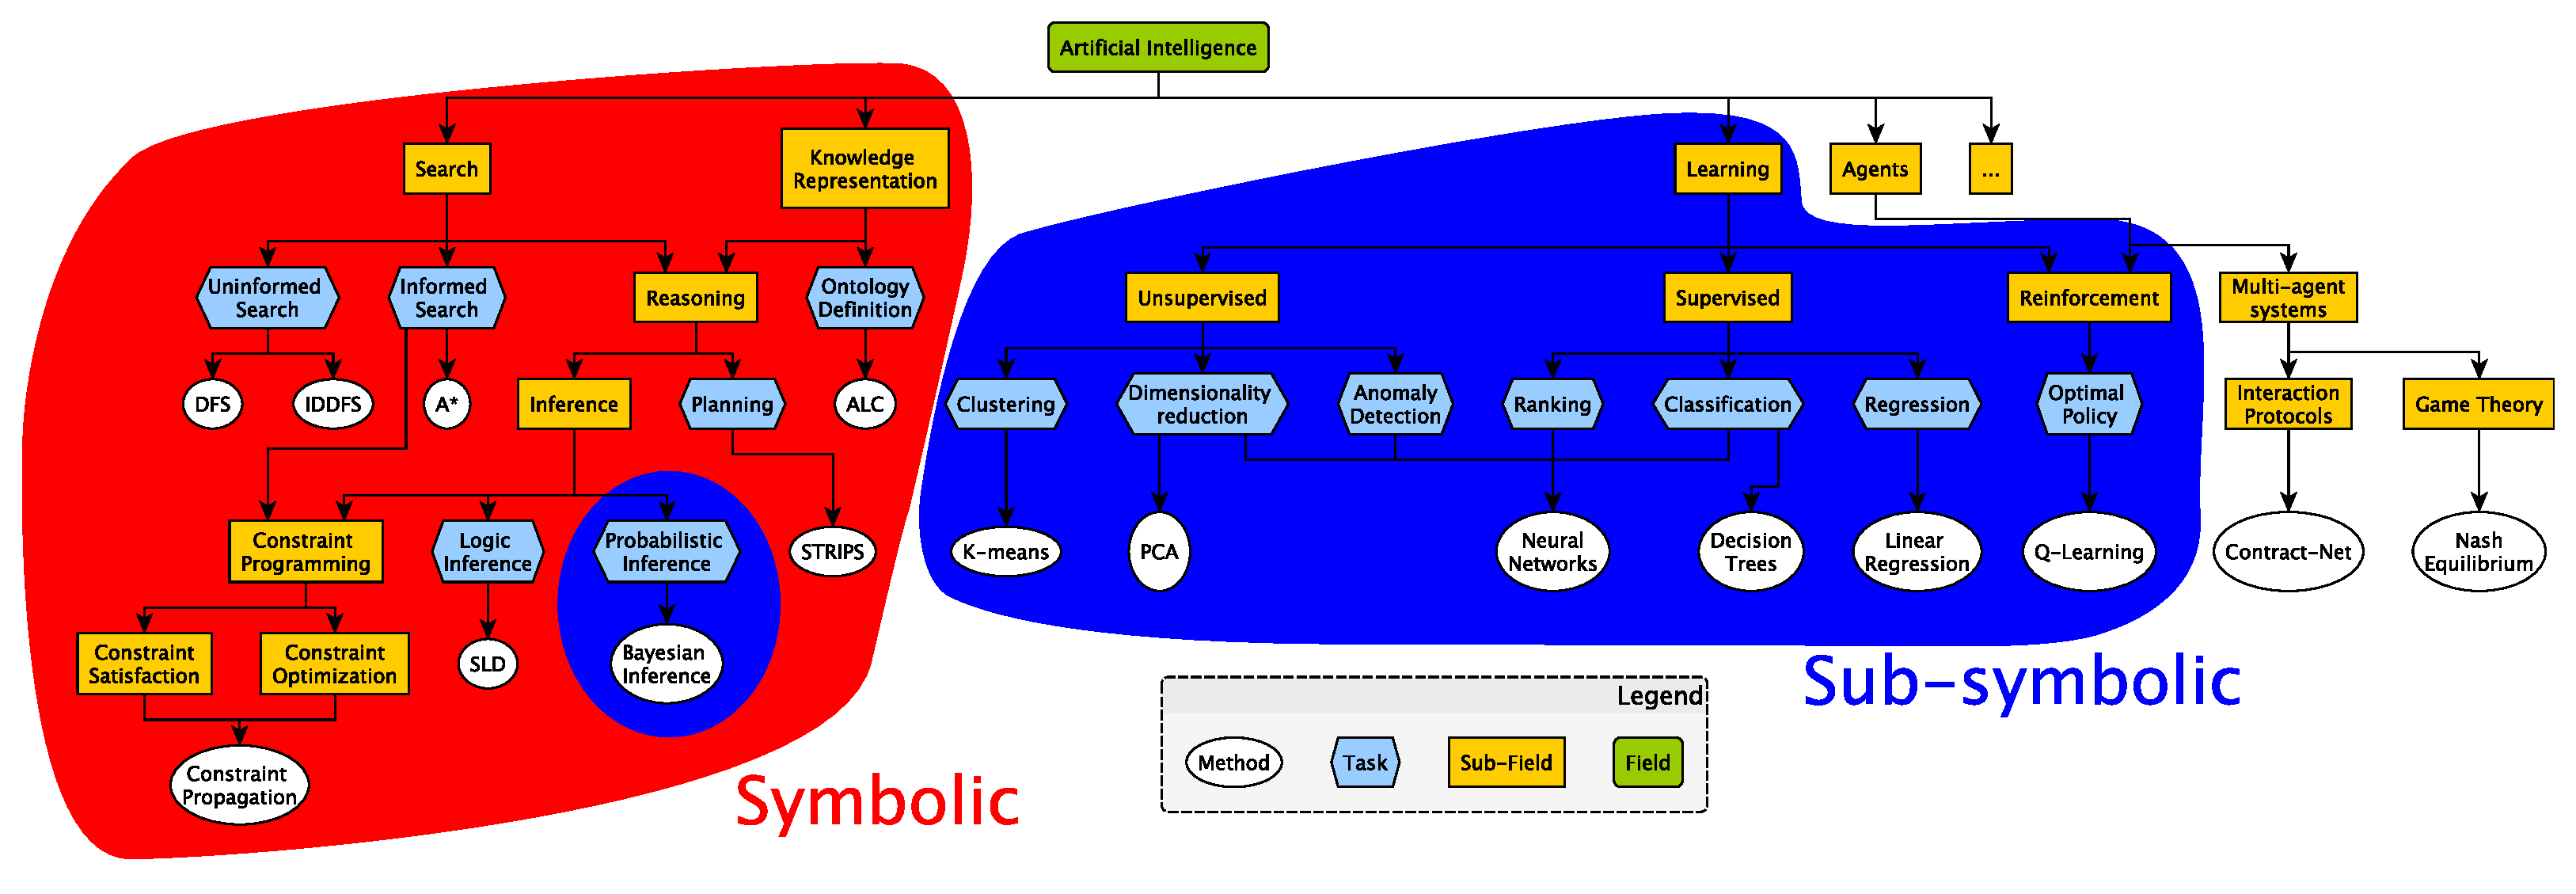
\includegraphics[width=\textwidth]{figures/ai-map2}
    \caption[Overview of the field of artificial intelligence]{
        \Gls{AI} map (not exhaustive) illustrating the main subfields with a focus on symbolic and sub-symbolic approaches.
        %
        On the left side, symbolic \gls{AI} is represented by search algorithms, \glspl{KR}, and reasoning.
        %
        On the right side, sub-symbolic \gls{AI} is represented by learning technique families, such as unsupervised learning, supervised learning, and reinforcement learning.
        %
        The figure is a simplified representation to give the reader a general idea of the landscape of \gls{AI}.
        %
        Notably, learning-based approaches are not necessarily subsymbolic.
        %
        For instance, \gls{ILP} and \glsentryshort{DT} learning induce explicit symbolic structures whose components retain a well-defined and compositional semantics, despite being learned from data.
    }
    \label{fig:ai-map}
\end{figure}


\paragraph{Local vs. distributed}
%
Multidimensional arrays are the fundamental building block of sub-symbolic data representation.
%
Formally, a $D$-order array is an ordered container of real numbers, where $D$ indicates the number of indices required to access each element.
%
We refer to 1-order arrays as \emph{vectors}, 2-order arrays as \emph{matrices}, and arrays of order greater than two as \emph{tensors}.
%
In sub-symbolic tasks based on arrays, information is typically conveyed both by the values stored in the array and their position within it.
%
The dimensions of the array -- denoted as $(d_1 \times \dots \times d_D)$ -- also play a crucial role, as sub-symbolic systems are usually designed to operate on arrays of fixed shape.
%
That is, the values of $d_1, \dots, d_D$ are chosen at design time and remain unchanged thereafter.
%
This violates \Cref{itm:symbolic-req-2} above; accordingly, we define sub-symbolic \gls{KR} as the task of encoding information into rigid numeric arrays.
%
\emph{Local} and \emph{distributed} representations are two key modes for encoding data into such arrays.
%
In local representations, each entry in the array corresponds to a well-defined concept from the target domain---its semantic meaning is clear and independent.
%
In distributed representations, by contrast, individual values carry little or no standalone meaning: their interpretation depends on the configuration of values across a neighbourhood in the indexing space.
%
Consequently, while the exact location of values is largely irrelevant in local representations, it becomes essential in distributed ones.
%
Notably, distributed representations violate \Cref{itm:symbolic-req-3}, and for this reason, recent literature often labels as \emph{sub-symbolic} those predictors that rely on distributed encoding of data.

%----------------------------------------------------------------------------------------
%------------------------------------ Symbolic AI ---------------------------------------
%----------------------------------------------------------------------------------------

\subsection[Symbolic AI]{Symbolic \Gls{AI}}\label{subsec:symbolic-ai}
%
Symbolic \gls{AI} has been regarded as crucial since \gls{AI}'s inception.
%
Symbolic \gls{KR} offers enhanced flexibility, expressiveness, and intelligibility, being interpretable both by machines and by humans.

\paragraph{Intentional vs. extensional}
%
In formal logic, one may define concepts either \emph{extensionally} or \emph{intensionally}.
%
Extensional definitions are direct representations of data.
%
For example, the set of square numbers admits the extensional definition $\{0,1,4,9,16,\dots\}$ by listing every member explicitly.
%
Conversely, an \emph{intensional} definition is an indirect representation of data.
%
In \gls{FOL}, this corresponds to defining a relation via a formula; for instance, the set of square numbers can be defined as $\{\,x\mid \exists n\in\mathbb{Z}\,(x = n^2)\}$ which succinctly encodes an infinite extension with a single schema.
%
Recursive intensional predicates further enhance expressivity: for example, the ancestor relation can be axiomatized by $\mathit{Ancestor}(x,y)\;\Leftrightarrow\;\mathit{Parent}(x,y)\;\lor\;\exists z\,[\,\mathit{Parent}(x,z)\wedge\mathit{Ancestor}(z,y)\,]$ allowing a compact representation of an infinite set of pairs with a finite rule.
%
In formal logic, intensional definitions are prized for their ability to model potentially unbounded domains within finite logical formalisms.


\paragraph{Expressiveness vs. tractability}
%
\begin{SCfigure}
    \centering
    \includegraphics[width=0.58\textwidth]{figures/venn_diagram_logics}
    \caption[Venn diagram of different logic families]{
        %
        Venn diagram of different logic families, illustrating the trade-off between expressiveness and tractability.
        %
        \Gls{FOL} is the most expressive logic -- not the most expressive logic in general -- encompassing all others.
        %
        On the other hand, propositional logic is the least expressive, as it can only represent atomic propositions and their combinations.
        %
        All the other logics fall somewhere in between, with varying degrees of expressiveness and tractability.
    }
    \label{fig:venn-diagram-logics}
\end{SCfigure}

%
Tractability addresses the theoretical question of whether a logic reasoner can determine the truth of a given formula within feasible time and space bounds.
%
The answer is deeply tied to the specific reasoning algorithm and the logic's formal properties.
%
Depending on the features a logic provides -- such as quantifiers, function symbols, or recursive definitions -- it may be more or less expressive.
%
The higher the expressiveness, the more complex the problems that can be represented and reasoned about, but this also increases the computational burden.
%
This well-known phenomenon is often referred to as the expressiveness/tractability trade-off~\cite{DBLP:journals/jlp/CadoliS93,BRACHMAN2004327,DBLP:journals/ci/LevesqueB87}.
%
In practice, highly expressive logics make it easier for human users to model rich domains, often requiring fewer and more concise formulas.
%
However, this comes at the cost of automated inference, which may become computationally intractable, undecidable, or non-terminating in the general case.
%
To mitigate this issue, various fragments and extensions of \gls{FOL} have been identified, each providing different tradeoffs between what can be expressed and what can be decided efficiently.
%
\Cref{fig:venn-diagram-logics} illustrates the relationships among different logic families, highlighting the trade-off between expressiveness and tractability.


\subsubsection[First-order logic]{\Glsentrylong{FOL}}\label{subsubsec:first-order-logic}
%
\Gls{FOL} is a general-purpose formalism that underpins most symbolic \gls{KR} systems.
%
It enables both human and computational agents to model entities and their interrelations through predicates and terms within a defined domain of discourse.
%
Its syntax comprises variables (quantified explicitly or implicitly), constants, function symbols, and predicate symbols, which are combined via logical operators such as conjunction (\(\wedge\)), disjunction (\(\vee\)), implication (\(\rightarrow\)), and equivalence (\(\leftrightarrow\)).
%
\Gls{FOL} allows for both \emph{extensional} and \emph{intensional} definitions.
%
Recursive intensional definitions, in particular, are powerful, enabling finite representations of infinite sets.
%
Despite its flexibility, \gls{FOL} is semi-decidable in general: there is no algorithm that can determine the truth of every \gls{FOL} formula in finite time, which limits its use in systems requiring guaranteed termination~\cite{DBLP:conf/dlog/2003handbook}.


\subsubsection{Horn logic}\label{subsubsec:horn-logic}
%
Horn logic is a significant subset of \gls{FOL}, offering a balanced trade-off between theoretical expressiveness and practical tractability~\cite{DBLP:journals/jcss/Makowsky87}.
%
It is built around the concept of \emph{Horn clauses}~\cite{DBLP:journals/jsyml/Horn51}, which are formulas in \gls{FOL} that exclude quantifiers and consist of a disjunction of predicates, with at most one non-negated literal.
%
Alternatively, a Horn clause can be expressed as an implication where the consequent is a single predicate and the antecedent is a conjunction of predicates: \(h \gets b_1, \dots, b_n\).
%
Here, \(\gets\) denotes logical implication (from right to left), commas represent logical conjunctions, and \(b_i\) as well as \(h\) are predicates of arbitrary arity, potentially containing \gls{FOL} terms such as variables, constants, or functions.

Horn clauses can be interpreted as \emph{if-then} rules written in reverse order, where only conjunctions of predicates are allowed in the antecedent.
%
In essence, Horn logic is a constrained subset of \gls{FOL} characterized by the following limitations:
%
\begin{inlinelist}
%
    \item formulas are reduced to clauses, containing only predicates, conjunctions, and a single implication operator;
    %
    \item operators such as \(\lor\), \(\leftrightarrow\), or \(\neg\) (negation) are not allowed;
    %
    \item variables are implicitly quantified; and
    %
    \item terms behave as they do in \gls{FOL}.
    %
\end{inlinelist}


\subsubsection{Datalog}\label{subsubsec:datalog}
%
Datalog is a declarative query language and a restricted subset of \gls{FOL}, designed for deductive databases and knowledge representation~\cite{DBLP:journals/jcss/AjtaiG94}.
%
It represents knowledge using function-free Horn clauses, as defined in \Cref{subsubsec:horn-logic}.
%
This restriction eliminates the use of function symbols, thereby forbidding structured terms such as recursive data structures.
%
As a result, Datalog is well-suited for applications requiring finite and decidable reasoning, as the absence of function symbols ensures termination of inference algorithms.
%
Similar to Horn logic, Datalog's knowledge bases consist of sets of function-free Horn clauses, which are interpreted as rules and facts.
%
Rules in Datalog follow the form \(h \gets b_1, \dots, b_n\), where \(h\) is the head of the rule and \(b_1, \dots, b_n\) are the body predicates.
%
Unlike general \gls{FOL}, Datalog does not allow disjunctions, negations, or explicit quantifiers, as variables are implicitly universally quantified.
%
Datalog is widely used in areas such as \glspl{KG}, semantic web technologies, and database systems, where efficient reasoning over large datasets is required.
%
Its simplicity and computational efficiency make it a practical choice for symbolic \gls{AI} tasks that demand tractable reasoning.


\subsubsection[Description logic]{\Glsentrylong{DL}}\label{subsubsec:dl}
%
\Gls{DL} are a family of subsets of \gls{FOL}, typically involving limited or no quantifiers, no structured terms, and no \textit{n}-ary predicates where \(n \geq 3\)~\cite{DBLP:books/daglib/0041477}.
%
In essence, \gls{DL} represents knowledge using constants and variables, along with atomic, unary, and binary predicates.


The differences among specific variants of \gls{DL} lie in the set of supported logical connectives and whether negation is allowed.
%
The wide variety of \gls{DL} stems from the well-known trade-off between expressiveness and tractability.
%
Depending on the application, one may prefer a more expressive \gls{DL} variant, which offers richer features at the cost of reduced tractability or even decidability of algorithms manipulating the knowledge, or vice versa.


In \gls{DL}, it is common practice to use specific terminology for different elements of knowledge representation:
%
\begin{itemize}
    %
    \item Constant terms are referred to as \textit{individuals}, as each constant represents a single entity within a domain.
    %
    \item Unary predicates are called \textit{classes} or \textit{concepts}, grouping sets of individuals for which the predicate holds true.
    %
    \item Binary predicates are referred to as \textit{properties} or \textit{roles}, connecting pairs of individuals.
    %
\end{itemize}
%

Using this nomenclature, knowledge in \gls{DL} can be represented by associating entities with constants (e.g., URLs) and defining concepts and properties accordingly.
%
Binary predicates are particularly significant as they enable the connection of pairs of entities.
%
This is typically achieved through subject-predicate-object triplets, represented as ground binary predicates of the form \(\langle a \, f \, b\rangle\) or \(f(a, b)\), where \(a\) is the subject, \(f\) is the predicate, and \(b\) is the object.

Collections of such triplets form \glspl{KG}, which are directed graphs where vertices represent individuals and arcs represent binary properties connecting these individuals.
%
\glspl{KG} may explicitly or implicitly instantiate a specific ontology, which is a formal description of classes characterizing a domain, their relationships (e.g., inclusion, exclusion, intersection, equivalence), and the properties they must or must not include.


\glspl{DL} are widely used in applications such as semantic web~\cite{DBLP:conf/coopis/GangemiM03} and ontology engineering~\cite{DBLP:books/ios/HGJKP2016}, where efficient reasoning and knowledge representation are essential.
%
Their ability to balance expressiveness and computational efficiency makes them a cornerstone of symbolic reasoning systems.


\subsubsection[Ontologies and knowledge graph]{Ontologies and \glsentrylong{KG}}\label{subsubsec:ontologies-and-kg}
%
An ontology is a formal and explicit specification of a shared conceptualisation of a domain~\cite{DBLP:books/daglib/p/Grimm10}.
%
It provides a structured vocabulary to describe the entities relevant in that domain, along with their attributes and the relationships among them.
%
This organisation enables both human understanding and machine-based reasoning.

Ontologies are typically expressed using \glspl{DL}, a family of logic-based formalisms for knowledge representation.
%
\Glspl{DL} define three main components:
%
\begin{inlinelist}
    %
    \item\emph{concepts} (or \emph{classes}), which group entities sharing similar features;
    %
    \item\emph{individuals} (or \emph{instances}), which are the concrete elements of the domain;
    %
    \item\emph{roles} (or \emph{properties}), which describe binary relationships between individuals.
    %
\end{inlinelist}
%
Different \glspl{DL} vary in their expressive power: for example, \gls{EL} supports only conjunction and existential quantification to ensure efficient reasoning, while more expressive DLs like \gls{ALC} allow for full Boolean operators and universal quantification.

Concepts are typically denoted using capital italic letters, such as $\mathit{Animal}$ or $\mathit{Cat}$.
%
These can be combined using logical constructors like intersection ($\sqcap$), union ($\sqcup$), or negation ($\lnot$) to form more complex classes.
%
A statement like $\mathit{Cat} \sqsubseteq \mathit{Animal}$ expresses that all cats are animals.

Individuals are constants representing specific entities in the domain and are usually written in monospaced lowercase, for example \texttt{tom}.
%
Membership of an individual in a concept is denoted using the ``is-a'' relation, written as \texttt{tom}~:~$\mathit{Cat}$, meaning ``Tom is a cat.''
%
Each individual may belong to multiple concepts.

Roles represent binary relations between individuals and are written in lowercase sans-serif font, such as \textsf{eats}.
%
They connect pairs of individuals, and their domain and range can be restricted using expressions such as $\textsf{eats} \sqsubseteq \mathit{Animal} \times \mathit{Edible}$.
%
Assertions like $\textsf{eats}(\texttt{tom}, \texttt{mouse})$ state that Tom eats the mouse.

The subsumption relation ($\sqsubseteq$) is used to express inclusion between concepts or roles.
%
For instance, $\mathit{Cat} \sqsubseteq \mathit{Animal}$ means that every cat is also an animal, and $\textsf{predatorOf} \sqsubseteq \textsf{eats}$ means that every predator-prey relationship implies eating.
%
Special concepts such as $\top$ and $\bot$ are used to denote the most general and the most specific concepts, respectively.

Collections of such axioms form an ontology.
%
\Gls{TBOX} define concepts and roles and their interrelations, while \gls{ABOX} specify which individuals belong to which concepts or are related via which roles.

\Glspl{KG} also provide a structured way to represent knowledge as graphs.
%
They consist of triplets (or \emph{facts}) of the form $(s, p, o)$, where $s$ is the subject, $p$ is the predicate (or property), and $o$ is the object.
%
These triplets form a directed graph where nodes represent individuals and edges represent relationships.

Unlike ontologies, KGs do not necessarily impose formal constraints on the structure or semantics of the triplets.
%
This flexibility allows for representing heterogeneous and incomplete data.
%
However, some \glspl{KG} are explicitly grounded in an ontology, and may follow its vocabulary and logical constraints.

In summary, ontologies and knowledge graphs both aim to formally capture structured knowledge.
%
Ontologies provide formal semantics and enable logical reasoning, while knowledge graphs emphasise scalability and flexibility in representing factual data.


\subsubsection{Propositional Logic}\label{subsubsec:propositional-logic}
%
Propositional logic is a restricted subset of \gls{FOL} in which quantifiers, terms, and non-atomic predicates are absent.
%
Its language consists solely of atomic propositions -- also called 0-ary predicates -- combined using standard logical connectives such as conjunction ($\land$), disjunction ($\lor$), negation ($\lnot$), and implication ($\rightarrow$).
%
Each proposition can be interpreted as a Boolean variable that takes a truth value in \{\texttt{true}, \texttt{false}\}.
%
The semantics of propositional logic aligns with Boolean algebra, making it straightforward to evaluate the truth of a formula given the truth values of its atomic components.

For example, a propositional formula such as $p \land \lnot q \rightarrow r$ can be interpreted as follows:
%
$p$ might stand for the proposition ``it is raining,'' $q$ for ``there is a roof,'' and $r$ for ``the floor is wet.''
%
In this case, the formula asserts that if it is raining and there is no roof, then the floor will be wet.

Compared to \gls{FOL}, propositional logic is significantly less expressive.
%
The absence of quantifiers means that general statements over a domain cannot be made.
%
Similarly, the lack of terms prevents direct reference to entities in the domain.
%
As a consequence, each relevant aspect of a scenario must be explicitly encoded as an individual proposition.

This limitation in expressiveness has important computational implications.
%
In particular, determining the satisfiability of a propositional formula is a decidable problem.
%
This makes propositional logic attractive in scenarios where tractable reasoning is required.

Despite its apparent simplicity, propositional logic can model a surprising range of situations.
%
Expressions involving numerical constants, variables, and comparisons (e.g., $x > 5$ or $y = 3$) can be encoded propositionally by introducing a distinct Boolean variable for each comparison.
%
This reduction allows the use of propositional logic in settings where the original problem does not explicitly involve logical variables or quantifiers, but can be decomposed into atomic truth conditions.


\subsubsection{Decision trees}\label{subsubsec:decision-trees}
%
\Glspl{DT} are a family of predictors that support both classification and regression tasks.
%
During the learning phase, the input space is recursively partitioned into multiple regions through a series of splits (i.e., decisions) based on the input data \(X\).
%
Each region is associated with a constant prediction, and the splits are designed to minimize the error with respect to the expected outputs \(Y\), while keeping the total number of regions low.
%
The learning process synthesizes a hierarchical structure of decision rules, which are followed to compute predictions for any \(x \in X\).
%
In the inference phase, these decision rules are evaluated sequentially, starting from the root of the tree and proceeding to a leaf node.
%
Each leaf corresponds to a specific region of the input space, resulting in a single prediction for each \(x\).

Unlike other predictor families, \glspl{DT} produce a tree of decision rules as the outcome of the learning process.
%
This tree is straightforwardly interpretable by humans and can be graphically represented in two-dimensional charts.
%
This property is particularly valuable when the internal workings of an automatic predictor need to be understood by a human agent.
%
\Glspl{DT} are often used in applications where interpretability is crucial, as their structure provides clear insights into the decision-making process.
%
They are often transformed into sets of logical rules for easier comprehension and analysis.


\subsubsection[Limits of symbolic AI]{Limits of symbolic \Gls{AI}}\label{subsubsec:limits-of-symbolic-ai}
%
Symbolic \gls{AI} has been a foundational approach in the field of \gls{AI}, providing a structured way to represent and reason about knowledge.
%
However, it also has several limitations.


Symbolic systems can be \emph{delicate}, meaning they may fail to handle unexpected situations or incomplete information~\cite{DBLP:books/ox/90/McDermott90}.
%
This is because symbolic systems rely on predefined rules and representations, which may not cover all possible scenarios.


As the complexity of the domain increases, the number of rules and symbols required to represent knowledge can grow significantly.
%
This can make it difficult to manage and maintain large symbolic systems; they do not \emph{scale} easily~\cite{DBLP:journals/ai/LenatF91}.


Symbolic systems typically require \emph{manual encoding} of knowledge, which can be time-consuming and error-prone.
%
This makes it challenging to adapt to new information or learn from experience.
%
This limitation is usually referred in the literature as the \emph{knowledge engineering bottleneck}~\cite{DBLP:books/aw/RN2020}.


Moreover, symbolic systems often struggle to handle \emph{uncertainty} and probabilistic reasoning.
%
This is because symbolic representations are typically deterministic, making it difficult to model real-world situations that involve uncertainty.


To sum up, symbolic models struggle to capture the nuances and complexities of real-world data, particularly when dealing with noisy or ambiguous information.
%
Also, they struggle when the domain is \emph{dynamic} and constantly changing, as they may require frequent updates to the rules and representations.


%-----------------------------------------------------------------------------------------
%------------------------------------ Sub-symbolic AI ------------------------------------
%-----------------------------------------------------------------------------------------

\subsection[Sub-symbolic AI]{Sub-symbolic \Gls{AI}}\label{subsec:sub-symbolic-ai}
%
Sub-symbolic \gls{AI} encompasses a wide range of techniques that rely on numerical representations.
%
Contributions come from varius fields, including \gls{ML}, statistical learning, and data mining.
%
The huge number of approaches is also motivated by the well known \gls{NFL} theorem~\cite{DBLP:journals/tec/DolpertM97} that states that no single learning algorithm can outperform all others across all possible tasks.
%
The most common predictor families are linear models, \glspl{DT}, \glspl{RF}, \glspl{SVM}, \glspl{NN} (including \glspl{LLM}), and many others.


\paragraph{Predictive performance vs. interpretability}
%
\begin{figure}[h]
    \centering
    \includegraphics[width=0.9\textwidth]{figures/interpretability-performance-tradeoff}
    \caption[Performance vs. interpretability trade-off]{
        %
        Trade-off between predictive performance and interpretability in common sub-symbolic predictors.
        %
        The figure illustrates how different predictor families balance these two aspects, with simpler models being more interpretable but potentially less accurate.
        %
    }
    \label{fig:performance-vs-interpretability}
\end{figure}
%
The \emph{complexity} of a sub-symbolic predictor can vary significantly.
%
By complexity we mean the overall structure of the model, including the number of parameters, the operations that are performed, and possibly the way the model is trained.
%
\Glspl{DT}, for example, are relatively simple models that can be easily interpreted by humans.
%
The downside of \glspl{DT} is that they make predictions by linearly partitioning the input space, which can lead to poor generalisation on unseen data.
%
On the other hand, \glspl{NN} can be extremely complex, with millions of parameters and intricate architectures that are difficult to interpret.
%
However, \glspl{NN} can capture highly non-linear relationships in the data, often leading to superior predictive performance compared to simpler models.
%
The definition of interpretability is not univocal, and it lacks measures that are widely accepted~\cite{DBLP:journals/natmi/Rudin19}.
%
Despite that, \Cref{fig:performance-vs-interpretability} illustrates in an informal way the trade-off between predictive performance and interpretability in sub-symbolic predictors.


\paragraph{Sort of \gls{ML} predictors}
%
There exist many sub-symbolic models in the literature.
%
Some of them are relatively simple and easy to interpret, while others are more complex and difficult to understand.
%
Among them, \gls{DT} are relatively simple, interpretable and popular models.
%
On the other hand, \glspl{NN} are more complex and difficult to interpret, but they can capture highly non-linear relationships in the data.
%
In between these two extremes, there are many other models, such as \glspl{RF} and \glspl{SVM}, that offer a balance between interpretability and predictive performance.
%
For the sake of conciseness, we will focus only on the models that are relevant for the rest of the thesis.


\subsubsection[Neural networks]{\Glsentrylongpl{NN}}\label{subsubsec:neural-networks}
%
\begin{figure}
    \centering
    \includegraphics[height=0.9\textheight]
    {figures/neural-network-architectures}
    \caption[Common neural network architectures]{
        %
        Overview of common \gls{NN} architectures.
        %
        Each architecture is designed to handle different types of data and tasks, leveraging specific structural features to improve performance.
    }
    \label{fig:nn-architectures}
\end{figure}
%
\Glspl{NN} are a family of predictors inspired by the structure and function of biological neural networks.
%
They consist of interconnected nodes -- a.k.a., neurons -- interconnected into a \gls{DAG} and organized into layers, where each neuron receives inputs, applies a non-linear activation function, and produces an output.
%
Despite being very popular nowadays, the first idea of a \gls{NN} has been proposed back in 1943~\cite{mcculloch1943logical}.
%
The so-called perceptron -- a single-layer \gls{NN} -- has been introduced in 1958~\cite{rosenblatt1958perceptron}.
%
Due to the limited expressiveness of single-layer \glspl{NN}, the perceptron could only learn linearly separable functions~\cite{DBLP:books/daglib/0066902}.

To overcome these limitations, researchers proposed to stack multiple layers of neurons, leading to the concept of \glspl{MLP}.
%
Although the theoretical foundations of such models were clear early on, the lack of an effective training algorithm hindered their practical use.
%
This changed with the rediscovery and popularization of the \textit{backpropagation} algorithm in the 1980s~\cite{rumelhart1986learning}, which allowed efficient computation of gradients through multiple layers using the chain rule of calculus.
%
This innovation enabled \glspl{MLP} to learn complex non-linear functions and marked the beginning of modern \gls{NN} research.

Many different architectures have been proposed since then, including fully connected \glspl{NN}, \glspl{CNN}, \glspl{RNN}, and more.
%
\Cref{fig:nn-architectures} provides an overview of some common \gls{NN} architectures.
%
These architectures are designed specifically to handle different types of data and tasks, such as image classification, \gls{NLP}, and time series analysis.


\paragraph{Feedforward Neural Networks}
%
The simplest class of \glspl{NN} is the family of feedforward networks, in which information flows unidirectional from the input layer through one or more hidden layers to the output layer, without forming cycles.
%
Among these, \glspl{MLP} are the canonical example, consisting of fully connected layers interleaved with non-linear activation functions.
%
Given sufficient capacity, \glspl{MLP} are universal function approximators~\cite{hornik1989multilayer}, capable of representing any Borel measurable function under mild assumptions.
%
Despite their theoretical expressiveness, \glspl{MLP} are inefficient when processing structured inputs such as images or sequences, as they fail to exploit the inherent inductive biases of the data.

\paragraph{Convolutional Neural Networks}
%
To overcome the limitations of \glspl{MLP} on grid-like data such as images, \glspl{CNN} were introduced.
%
Pioneering work on hierarchical feature extraction was done by Fukushima with the Neocognitron~\cite{fukushima1980neocognitron}, followed by the successful application of convolutional networks to handwritten digit classification in LeNet-5~\cite{lecun1998gradient}.
%
\glspl{CNN} apply learnable convolutional filters that exploit local spatial correlations, reducing the number of parameters and enabling translation equivariance.
%
Pooling layers further promote translation invariance by down sampling intermediate representations.
%
These properties make \glspl{CNN} particularly well-suited for tasks involving visual perception.

\paragraph{Recurrent Neural Networks}
%
\Glspl{RNN} are designed to process sequential data by incorporating recurrence in the form of feedback connections.
%
More generally, recurrence in neural networks refers to the presence of cyclic connections that give rise to an internal state evolving over time, allowing the network to be interpreted as a discrete-time dynamical system.
%
From this perspective, the current state of the network depends not only on the current input but also on its previous state, enabling the modelling of temporal dependencies and variable-length input sequences.
%
In standard \glspl{RNN} architectures, this recurrent behaviour is typically implemented by units that receive input both from the current time step and from their own past activations, effectively providing a form of memory across time.
%
Despite their expressive power, standard \glspl{RNN} suffer from the vanishing and exploding gradient problems~\cite{bengio1994learning}, which hinder their ability to learn long-range dependencies.
%
To address these issues, more sophisticated variants have been developed, notably \glspl{LSTM}~\cite{hochreiter1997long} and \glspl{GRU}~\cite{cho2014learning}, which introduce gating mechanisms to regulate information flow and preserve long-term context.


\subsubsection{\Glsentrylong{LLM}}\label{subsubsec:llm}
%
Pre-trained \glspl{LLM}, such as the GPT models developed by OpenAI~\cite{radford2018improving}, have achieved remarkable success in various \gls{NLP} tasks.
%
These models, based on the \emph{transformer} architecture~\cite{DBLP:conf/nips/VaswaniSPUJGKP17}, are trained on vast amounts of textual data, enabling them to encode extensive knowledge about real-world entities, such as historical events and geographical facts~\cite{DBLP:journals/tacl/JiangXAN20}.
%
They can perform tasks like lexical operations, common-sense reasoning, and solving mathematical problems~\cite{DBLP:conf/emnlp/MadasuS22,DBLP:journals/tacl/GevaKSKRB21,DBLP:conf/nips/Wei0SBIXCLZ22}.
%
However, the extent to which \glspl{LLM} exhibit genuine reasoning abilities remains a topic of debate~\cite{DBLP:journals/ethicsit/HicksHS24}.
%
Some studies suggest that these models often rely on statistical patterns in the data to simulate reasoning, rather than truly understanding the underlying concepts~\cite{DBLP:conf/fat/BenderGMS21}.
%
% This debate highlights the need for further research into the interpretability and reasoning capabilities of \glspl{LLM}.

The transformer architecture, introduced by Vaswani et al.~\cite{DBLP:conf/nips/VaswaniSPUJGKP17}, was originally designed for machine translation.
%
Over time, it has become the foundation for state-of-the-art \gls{NLP} models.
%
A transformer consists of two main components: the \emph{Encoder}, which converts a text sequence into an embedded representation, and the \emph{Decoder}, which generates output sequences in an autoregressive manner.
%
Both components are composed of multiple layers, with each layer incorporating mechanisms like self-attention and feed-forward neural networks.

The self-attention mechanism is a key innovation of the transformer.
%
It allows the model to focus on different parts of a sentence, capturing contextual relationships between words.
%
Formally, given an embedded representation \(E\), the model computes three vectors: \emph{key} (\(K\)), \emph{query} (\(Q\)), and \emph{value} (\(V\)), using weight matrices \(W_k\), \(W_q\), and \(W_v\).
%
The output is then calculated as:
%
\[
Z = \text{softmax}\left(\frac{QK^\top}{\sqrt{d_k}}\right)V,
\]
%
where \(d_k\) is the dimensionality of the key vectors.
%
This mechanism is extended to multiple attention heads in the \emph{Multi-Head Attention} module, enhancing the model's ability to capture diverse relationships.

Two prominent transformer-based models are BERT and GPT.
%
BERT, introduced in~\cite{DBLP:conf/naacl/DevlinCLT19}, is an encoder-based model trained using \emph{masked language modeling}, where certain words in the input are masked, and the model predicts them.
%
In contrast, GPT~\cite{radford2018improving} is a decoder-based model trained with \emph{causal language modeling}, generating text sequentially from a given prefix.
%
These models have set benchmarks in various \gls{NLP} tasks, demonstrating the versatility and power of transformer architectures.


\paragraph{Learning from the Web}

\glspl{LLM} can be viewed as extensive \emph{knowledge bases}~\cite{PetroniRRLBWM19}.
%
They store the textual data they were trained on and enable efficient information retrieval through free-text queries.
%
The training data for these models is typically sourced from a wide range of publicly available Web content.

%
For example, the early BERT model~\cite{DBLP:conf/naacl/DevlinCLT19} was trained on the BooksCorpus dataset~\cite{ZhuKZSUTF15}, a collection of over 11,000 books, and a snapshot of the English Wikipedia.
%
Similarly, GPT~\cite{gpt2-2019,gpt3-2020} were trained on datasets scraped from the public Internet, using Reddit as an entry point for identifying high-quality content~\cite{training-data-attack-2021}.
%
The RoBERTa model~\cite{roberta-2019} extended this approach by incorporating additional datasets, such as:
%
\begin{inlinelist}
    \item the Common~Crawl News dataset\footnote{\url{https://commoncrawl.org}},
    %
    \item the OpenWebTextCorpus~\cite{Gokaslan2019OpenWeb}, and
    %
    \item the Stories dataset~\cite{TrieuQuoc2018}.
\end{inlinelist}

%
The LLAMA family of models~\cite{llama1,llama2} utilized a combination of datasets, including the colossal clean crawled corpus (C4)~\cite{RaffelSRLNMZLL20}, English Wikipedia, and other sources.
%
Finally, the Mixtral-of-Experts model by MistralAI is also pre-trained on data extracted from the open Web\footnote{\url{https://mistral.ai/news/mixtral-of-experts}}.


\paragraph{Oracles for Data Generation}
%
Web-based pre-training allows \glspl{LLM} to accumulate substantial domain-specific knowledge across a wide range of topics.
%
This knowledge can be extracted by crafting appropriate prompts, enabling \glspl{LLM} to act as \emph{oracles} for information retrieval tasks.
%
Such capabilities are particularly useful for generating synthetic data that incorporates domain-specific knowledge.
%
In these cases, users can design prompts to guide the \gls{LLM} in generating the desired content, which can then be converted into the required format.


\paragraph{Hallucinations}
%
It is important to note that \glspl{LLM} are not perfect oracles.
%
They may produce text that is factually incorrect or inconsistent with the context, a phenomenon known as \emph{hallucination}~\cite{hallucination-2023}.
%
This limitation highlights the need for careful evaluation of the outputs generated by \glspl{LLM}, as they cannot be blindly trusted.

%
\paragraph{Temperature}
%
To mitigate hallucinations, \glspl{LLM} often include a parameter called \emph{temperature}, which controls the randomness of their responses.
%
The temperature parameter is a real value in the range \([0, 1]\).
%
A lower temperature results in more deterministic outputs, as the model selects the most probable next word.
%
Conversely, a higher temperature introduces more randomness by sampling from the probability distribution of possible next words.
%
This mechanism allows users to balance the \emph{creativity} of the model with the need for accuracy\footnote{
    %
    A language model predicts the next word in a sequence based on a probability distribution.
    %
    Setting the temperature to 0 ensures deterministic outputs by always selecting the most likely word, while a temperature of 1 introduces randomness by sampling from the distribution.
}.


\paragraph{The Role of Prompts}

Another approach to address hallucinations is \emph{prompt engineering}.
%
Clear and unambiguous prompts can help align the \gls{LLM}'s output with user expectations.
%
For instance, explicitly instructing the \gls{LLM} to adopt the perspective of a domain expert has been shown to improve the accuracy of its responses~\cite{MemmertCB24}.
%
Additionally, asking the model to ``work step-by-step'' can enhance the quality of procedural descriptions~\cite{YangWLLZC23}.


\subsubsection[Limits of sub-symbolic AI]{Limits of sub-symbolic \Gls{AI}}\label{subsubsec:limits-of-sub-symbolic-ai}
%
Sub-symbolic \gls{AI} has achieved remarkable success in various domains and scenarios, but it also has limitations.


One of the main limitations is the need for \emph{large amounts} of training data if the predictive task is not trivial (e.g., easy to linearly separate).
%
Sub-symbolic models, especially deep learning models, often require vast amounts of labeled data to learn effectively~\cite{DBLP:journals/nature/LeCunBH15}.
%
This can be a significant challenge in domains where data is scarce or expensive to obtain.


Another limitation is the \emph{lack of interpretability}.
%
Sub-symbolic models, particularly deep learning models, are often considered black boxes because their internal workings are not easily understandable by humans~\cite{DBLP:journals/natmi/Rudin19,interpretability-lipton-2018}.
%
This is a significant drawback in applications where transparency and explainability are crucial, such as healthcare and finance.


Sub-symbolic models can also be sensitive to \emph{adversarial attacks}, where small perturbations to the input data can lead to incorrect predictions~\cite{DBLP:journals/corr/SzegedyZSBEGF13}.
%
This vulnerability raises concerns about the robustness and security of sub-symbolic \gls{AI} systems.


Additionally, sub-symbolic models may struggle to \emph{generalize to out-of-distribution data}, meaning they may perform poorly when faced with inputs that differ significantly from the training data~\cite{DBLP:conf/icml/RechtRSS19}.
%
Finally, sub-symbolic models often lack common-sense reasoning abilities, making it difficult for them to understand and reason about the world in a way that humans do.


%-----------------------------------------------------------------------------------------
%----------------------------------- AI and society --------------------------------------
%-----------------------------------------------------------------------------------------

\section{AI and society}\label{sec:ai-and-society}
%
This last section of the chapter is needed to introduce \gls{AI} sub-fields that have become increasingly important in recent years.
%
In particular, the consequences of the wide adoption of \gls{AI} systems in everyday life have raised concerns about their trustworthiness, fairness, and accountability.
%

\subsection[Explainable AI]{\Glsentrylong{XAI}}\label{subsec:xai}
%
Modern intelligent systems increasingly rely on sub-symbolic predictive models to support their intelligent behaviour.
%
These models are typically trained using a data-driven approach, leveraging the vast availability of data generated in recent years.
%
\Gls{ML} algorithms enable the semi-automatic detection of statistical patterns hidden within data.
%
Such patterns can then be used to support decision-making, planning, and forecasting across various domains where data is available.


Despite their predictive capabilities, \gls{ML} models face significant challenges in critical applications.
%
One of the most notable issues is \emph{algorithmic opacity}, which refers to the difficulty humans face in understanding how these models operate or make decisions.
%
Opacity arises due to the complex interplay between high-dimensional datasets, the algorithms processing them, and the dynamic behaviour of these algorithms during training~\cite{DBLP:journals/bigdatasociety/Burrell16}.
%
This lack of transparency is particularly problematic in domains such as healthcare, finance, and law, where human accountability and explainability are essential.


The term \emph{black box} is often used to describe \gls{ML} predictors, as their internal workings are not symbolically represented~\cite{interpretability-lipton-2018}.
%
Without symbolic representations, it becomes challenging for humans to comprehend the operation of these systems or the rationale behind their decisions.
%
This can lead to a lack of trust and acceptance of \gls{AI}-based solutions.


Regulatory frameworks, such as the \gls{GDPR}, have started to recognise the \emph{right to explanation}~\cite{DBLP:journals/aim/GoodmanF17}.
%
This right mandates that intelligent systems must be understandable to ensure fairness, identify biases, and verify that they function as intended.
%
However, the concept of \emph{understandability} remains neither standardised nor systematically assessed~\cite{DBLP:journals/ai/Miller19}.
%
While some \gls{ML} models are more interpretable than others, there is no consensus on what constitutes an adequate explanation.


Interpretability and explainability are desirable properties for intelligent systems.
%
\Gls{XAI} aims to make sub-symbolic \gls{AI} more interpretable for humans, often by automating the generation of explanations.
%
Interpretability refers to the cognitive effort required by humans to assign meaning to the behaviour or outcomes of intelligent systems.
%
It is often associated with properties such as algorithmic transparency, decomposability, and predictability.


An \emph{explanation}, on the other hand, is a set of statements or accounts that clarify an object or justify an action.
%
Explanations can involve constructing more interpretable representations of a black-box model.
%
For instance, \emph{model simplification} techniques translate a complex model into a simpler one with high fidelity~\cite{DBLP:conf/kdd/TolomeiSHL17,DBLP:journals/csur/GuidottiMRTGP19}.
%
Alternatively, symbolic knowledge can be extracted from sub-symbolic predictors, producing interpretable objects from less interpretable ones.


Another approach to improving interpretability involves injecting symbolic knowledge into sub-symbolic predictors.
%
This process does not produce explanations but increases the model's transparency by aligning its behaviour with more interpretable systems.

Interpretability and explainability enhance trustworthiness in \gls{AI}-based solutions.
%
However, they also enable users to exercise finer control over these systems, deciding whether to trust them or not~\cite{10.1214/21-SS133}.
%
The surveyed \gls{SKE} and \gls{SKI} methods should be regarded as tools for increasing user control over \gls{AI} systems.


\subsubsection{Sorts of Explanation}\label{subsubsec:sorts-of-explanation}
%
Two major approaches exist to bring explainability or interpretability to intelligent systems: \emph{by design} and \emph{post-hoc}~\cite{DBLP:conf/atal/CiattoSOC20,DBLP:journals/inffus/ArrietaRSBTBGGM20,DBLP:journals/csur/GuidottiMRTGP19}.


\paragraph{\Gls{XAI} by Design}
\label{par:xai-by-design}
%
This approach aims to make systems interpretable or explainable from the outset, treating these features as primary design goals.
%
Methods in this category can be further divided into:
%
\begin{itemize}
    \item \emph{Symbols as constraints}, where predictive models are constrained by symbolic rules, often expressed in subsets of \gls{FOL}.
    \item \emph{Transparent box design}, where models are inherently interpretable and require no further manipulation.
\end{itemize}

\paragraph{Post-hoc Explainability}
%
This approach involves manipulating pre-existing systems to make them interpretable or explainable.
%
Methods in this category include:
%
\begin{itemize}
    \item \emph{Text explanation}, which generates textual descriptions of model behaviour.
    \item \emph{Visual explanation}, which visualises model behaviour, often using dimensionality reduction techniques.
    \item \emph{Local explanation}, which segments the solution space into simpler subspaces and explains them.
    \item \emph{Explanation by example}, which extracts representative examples to illustrate internal relationships.
    \item \emph{Model simplification}, which constructs a simplified system that optimises similarity to the original while reducing complexity.
    \item \emph{Feature relevance}, which assigns relevance scores to features, revealing their importance in the model's output.
\end{itemize}


\subsection[Fairness in AI]{Fairness in \gls{AI}}
\label{subsec:fairness-in-ai}
%
\Gls{ML} models can inherit and amplify biases present in the dataset \(D\).
%
For instance, if \(D\) contains features related to gender or race, and the data is not equally distributed across these groups, biases may arise.
%
This often occurs in datasets about hiring decisions, where historical data may reflect fewer non-male or non-white candidates.
%
A supervised model \(H\), trained on such a dataset to predict a target feature \(Y\), might incorrectly learn that gender or race influences the prediction.
%
If the predictions of \(H\) are used for decision-making, such as hiring or loan approvals, the model may discriminate against certain groups.
%
In this case, the model is said to be biased, as it replicates patterns of past discrimination.

%
Fairness interventions can mitigate these biases and are applied at different stages of the \gls{ML} workflow.
%
In the literature, these methods are categorized as:
%
\begin{itemize}
    \item \textit{Pre-processing methods}, which modify the dataset \(D\) to reduce bias before training;
    %
    \item \textit{In-processing methods}, which adjust the learning algorithm \(A\) to enforce fairness during training;
    %
    \item \textit{Post-processing methods}, which modify the predictions of the model \(H\) to achieve fairness after training.
\end{itemize}

%
A critical prerequisite for fairness interventions is the ability to measure fairness.
%
Fairness metrics quantify the extent of bias in a dataset or model and evaluate the effectiveness of mitigation techniques.
%
Formally, a fairness metric is a function that takes data as input and returns a numerical score.
%
The input data can be a dataset \(D = (X, Y)\) or the predictions \(h(X)\) of a model on \(D\).
%
A lower score typically indicates higher bias, while a higher score reflects greater fairness.

%
Numerous fairness metrics have been proposed, differing in the type of data they accept and their interpretation of fairness or bias.
%
These metrics are often categorized based on the fairness notion they adhere to~\cite{DBLP:journals/csur/MehrabiMSLG21}.
%
The two most common notions are \textit{group fairness} and \textit{individual fairness}.


\paragraph{Group fairness}\label{par:group-fairness}
%
Group fairness ensures that distinct groups of individuals, defined by sensitive attributes, are treated equally.
%
Sensitive attributes, denoted as \( S \subset X \), are features such as \emph{gender}, \emph{race}, \emph{age}, or social status, which partition the dataset \( D \) into protected groups.
%
These groups can be defined by a single sensitive attribute, e.g., the group of women identified by a specific value of the \textit{gender} feature, or by a combination of attributes, e.g., the group of Black women identified by both \textit{gender} and \textit{race}.
%
The principle of group fairness is commonly evaluated by measuring the correlation between sensitive attributes \( S \) and the target variable \( Y \).
%
For instance, if \( Y \) represents loan approval outcomes and \( S \) represents the applicant's race, group fairness metrics assess whether the approval rates are consistent across racial groups.
%
Such metrics are crucial for identifying and addressing biases in decision-making processes.


\paragraph{Individual fairness}\label{par:individual-fairness}
%
Individual fairness ensures that similar individuals receive similar treatment.
%
The simplest approach to individual fairness is \emph{fairness through awareness}.
%
This method relies on a distance metric \(\delta : X \times X \to \mathbb{R}\) in the input space (e.g., Euclidean distance).
%
It requires that if two individuals \(x_1\) and \(x_2\) are similar up to a threshold \(\epsilon\), i.e., \(\delta(x_1, x_2) < \epsilon\), then their corresponding target values \(y_1\) and \(y_2\) should also be similar.
%
In practice, model predictions \(h(x_1)\) and \(h(x_2)\) are compared instead of true labels, and fairness scores are computed by averaging the differences in predictions for similar instances.
%
Another approach is \emph{fairness through unawareness}, which requires that sensitive attributes are not used by the model during training or prediction.
%
This can be achieved by removing sensitive features from the dataset or ensuring the model does not rely on them.
%
Fairness scores in this case measure the extent to which the model depends on sensitive attributes and penalize such reliance.
%
A more advanced formulation is \emph{counterfactual fairness}.
%
This requires that a model's prediction for an individual \(x\) remains the same, regardless of whether \(x\) belongs to a group \(s\) in the actual dataset or to a counterfactual group \(s' \neq s\).
%
Counterfactual fairness ensures that predictions are invariant to changes in sensitive attributes across hypothetical scenarios.
%
As individual fairness is not the primary focus of this work, we do not delve into the specific metrics used to evaluate it.
%
For a detailed discussion, the reader is referred to~\cite{DBLP:journals/csur/MehrabiMSLG21}.

%%! Author = matteomagnini
%! Date = 05/03/25

%----------------------------------------------------------------------------------------
\chapter[Artificial Intelligence]{\Glsentrylong{AI}}
\label{ch:ai}
\minitoc
%----------------------------------------------------------------------------------------

\section{Overview}\label{sec:ai-overview}
%
The wide range of \gls{AI} techniques used to be divided into two main categories: \emph{symbolic} and \emph{sub-symbolic} \gls{AI}.
%
The thing that distinguishes the two categories is the way they \emph{represent knowledge} and how they process it.
%
No intelligence can exist without knowledge and no computation can occur in lack of representation.
%
In the rest of the thesis, we will use the term symbolic (resp., sub-symbolic) \gls{AI} and symbolic (resp., sub-symbolic) \gls{KR} almost interchangeably.
%
Symbolic \gls{AI} is based on \emph{symbols}, which come with a \emph{meaning} and could be manipulated according to the formalism and rules of a given \gls{AI} system.
%
On the other hand, sub-symbolic \gls{AI} is based on a numerical representation -- a.k.a., sub-symbolic -- where the numbers are not directly interpretable.
%
Numbers are technically symbols, but numbers, arrays and their functions are not recognised as means for symbolic \gls{KR}.
%
According to Van Gelder~\cite{DBLP:conf/ogai/Gelder90}, in order to be considered symbolic, \gls{KR} approaches must:
%
\begin{requirements}
    %
    \item \label{itm:symbolic-req-1} involve a set of symbols;
    %
    \item \label{itm:symbolic-req-2} the symbols can be combined following a set of grammatical rules;
    %
    \item \label{itm:symbolic-req-3} elementary symbols and combinations of symbols can be assigned a meaning.
    %
\end{requirements}


\paragraph{Local vs. distributed}
%
Multidimensional arrays are the fundamental building block of sub-symbolic data representation.
%
Formally, a $D$-order array is an ordered container of real numbers, where $D$ indicates the number of indices required to access each element.
%
We refer to 1-order arrays as \emph{vectors}, 2-order arrays as \emph{matrices}, and arrays of order greater than two as \emph{tensors}.
%
In sub-symbolic tasks based on arrays, information is typically conveyed both by the values stored in the array and their position within it.
%
The dimensions of the array -- denoted as $(d_1 \times \dots \times d_D)$ -- also play a crucial role, as sub-symbolic systems are usually designed to operate on arrays of fixed shape.
%
That is, the values of $d_1, \dots, d_D$ are chosen at design time and remain unchanged thereafter.
%
This violates \Cref{itm:symbolic-req-2} above; accordingly, we define sub-symbolic \gls{KR} as the task of encoding information into rigid numeric arrays.
%
\emph{Local} and \emph{distributed} representations are two key modes for encoding data into such arrays~\cite{hinton1986learning}.
%
In local representations, each entry in the array corresponds to a well-defined concept from the target domain---its semantic meaning is clear and independent.
%
In distributed representations, by contrast, individual values carry little or no standalone meaning: their interpretation depends on the configuration of values across a neighbourhood in the indexing space.
%
Consequently, while the exact location of values is largely irrelevant in local representations, it becomes essential in distributed ones.
%
Notably, distributed representations violate \Cref{itm:symbolic-req-3}, and for this reason, recent literature often labels as \emph{sub-symbolic} those predictors that rely on distributed encoding of data.


\section{Symbolic \Gls{AI}}\label{sec:symbolic-ai}
%
Symbolic \gls{AI} has been regarded as crucial since \gls{AI}'s inception.
%
Symbolic \gls{KR} offers enhanced flexibility, expressiveness, and intelligibility, being interpretable both by machines and by humans.

\paragraph{Intentional vs. extensional}
%
In formal logic, one may define concepts either \emph{extensionally} or \emph{intensionally}.
%
Extensional definitions are direct representations of data.
%
For example, the set of square numbers admits the extensional definition $\{0,1,4,9,16,\dots\}$ by listing every member explicitly.
%
Conversely, an \emph{intensional} definition is an indirect representation of data.
%
In \gls{FOL}, this corresponds to defining a relation via a formula; for instance, the set of square numbers can be defined as $\{\,x\mid \exists n\in\mathbb{Z}\,(x = n^2)\}$ which succinctly encodes an infinite extension with a single schema.
%
Recursive intensional predicates further enhance expressivity: for example, the ancestor relation can be axiomatized by $\mathit{Ancestor}(x,y)\;\Leftrightarrow\;\mathit{Parent}(x,y)\;\lor\;\exists z\,[\,\mathit{Parent}(x,z)\wedge\mathit{Ancestor}(z,y)\,]$ allowing a compact representation of an infinite set of pairs with a finite rule.
%
In formal logic, intensional definitions are prized for their ability to model potentially unbounded domains within finite logical formalisms.


Historically, most \gls{KR} formalisms and their enabling technologies have been rooted in \gls{CL}.
%
Notable examples, for instance, include \gls{FOL}, \gls{HL}, \gls{DL}, and ontologies.
%
Increased expressiveness often comes at the cost of higher computational complexity, giving rise to the well-known \emph{expressiveness vs. tractability} trade-off~\cite{DBLP:conf/dlog/2003handbook}.
%
To balance these concerns, various fragments and extensions of \gls{FOL} have been identified, each providing different tradeoffs between what can be expressed and what can be decided efficiently.


\paragraph{Expressiveness vs. tractability}
%
Tractability addresses the theoretical question of whether a logic reasoner can determine the truth of a given formula within feasible time and space bounds.
%
The answer is deeply tied to the specific reasoning algorithm and the logic's formal properties.
%
Depending on the features a logic provides -- such as quantifiers, function symbols, or recursive definitions -- it may be more or less expressive.
%
The higher the expressiveness, the more complex the problems that can be represented and reasoned about, but this also increases the computational burden.
%
This well-known phenomenon is often referred to as the expressiveness/tractability trade-off~\cite{DBLP:journals/jlp/CadoliS93,BRACHMAN2004327,DBLP:journals/ci/LevesqueB87}.
%
In practice, highly expressive logics make it easier for human users to model rich domains, often requiring fewer and more concise formulas.
%
However, this comes at the cost of automated inference, which may become computationally intractable, undecidable, or non-terminating in the general case.
%
To mitigate this issue, many systems adopt restricted fragments of first-order logic—such as Horn clauses or decidable Description Logics—that preserve a useful degree of expressiveness while maintaining decidability and, often, practical efficiency~\cite{lloyd1987foundations,baader2003description}.



\subsection{\Glsentrylong{FOL}}\label{subsec:first-order-logic}

\subsection{\Glsentrylong{DL}}\label{subsec:dl}

\subsection{Ontologies}\label{subsec:ontologies}

\subsection{Horn logic}\label{subsec:horn-logic}

\subsection{Expert Systems}\label{subsec:expert-systems}

\subsection{Trees and other algorithms}\label{subsec:trees-and-other-algorithms}

\subsection{Limits of symbolic \Gls{AI}}\label{subsec:limits-of-symbolic-ai}

\section{Sub-symbolic \Gls{AI}}\label{sec:sub-symbolic-ai}

\subsection{Random forests}\label{subsec:random-forests}

\subsection{Bayesian methods}\label{subsec:bayesian-methods}

\subsection{Evolutionary algorithms}\label{subsec:evolutionary-algorithms}

\subsection{\Glsentrylongpl{SVM}}\label{subsec:svm}

\subsection{\Glsentrylongpl{NN}}\label{subsec:neural-networks}

\subsection{Limits of sub-symbolic \Gls{AI}}\label{subsec:limits-of-sub-symbolic-ai}
%! Author = matteomagnini
%! Date = 05/03/25

%----------------------------------------------------------------------------------------
\chapter{Neuro-symbolic AI}
\label{ch:nesy-ai}
\minitoc
%----------------------------------------------------------------------------------------

The origins of \gls{NeSy} \gls{AI} can be traced back to the 1950s and 1960s, during the early days of \gls{AI} research~\cite{Youheng_2023}.
%
At that time, the focus was on developing systems based on symbolic reasoning and rule-based problem-solving.
%
However, by the 1980s, the limitations of purely symbolic approaches became evident.
%
For instance, symbolic \gls{AI} struggled with tasks such as \gls{NLP} and computer vision, where the complexity of real-world data posed significant challenges.
%
To address these shortcomings, researchers began incorporating principles inspired by neuroscience into \gls{AI} systems.
%
This shift marked the beginning of efforts to integrate sub-symbolic methods, such as neural networks, into the field.

In the early 21st century, the idea of combining symbolic reasoning with neural networks gained traction.
%
This led to the emergence of \gls{NeSy} \gls{AI}, a hybrid approach that leverages the strengths of both symbolic and sub-symbolic paradigms.


\Gls{NeSy} \gls{AI} has since been applied to a wide range of domains, including healthcare, robotics, and \gls{NLP}.
%
It represents one of the most promising directions in \gls{AI} research, aiming to create systems capable of both learning from data and reasoning logically, much like humans.
%
The ``neuro'' component of \gls{NeSy} \gls{AI} is inspired by the human brain's ability to process information and learn from experience.
%
This is achieved through the use of neural networks, which enable the system to adapt and generalize from data.
%
On the other hand, the ``symbolic'' component relies on logical reasoning and structured representations of knowledge.
%
This allows the system to perform tasks such as deductive reasoning and to represent knowledge in a human-interpretable form, using symbols and rules.
%
By combining these two components, \gls{NeSy} \gls{AI} aims to overcome the limitations of purely symbolic or sub-symbolic approaches.
%
It enables the development of intelligent systems that can reason, learn, and adapt in complex environments.


According to a recent survey~\cite{DBLP:journals/nca/BhuyanRTS24} there exist at least six different types of integrating symbolic \gls{AI} and sub-symbolic \gls{ML} predictors.
%
Approaches to \gls{NeSy} can be categorised w.r.t. how the connectionist and symbolic components are integrated.
%
\begin{enumerate}
    \item \emph{Symbolic neuro-symbolic} (Type 1): utilizes neural networks for representational learning, which subsequently feeds into symbolic logic and inference mechanisms.
    %
    This approach is particularly effective in tasks such as language translation and classification, where neural-based semantic representations enhance symbolic reasoning;
    %
    \item \emph{symbolic[neuro]} (Type 2): incorporates neural networks as subcomponents within predominantly symbolic frameworks.
    %
    This integration improves pattern recognition capabilities within symbolic reasoning systems;
    %
    \item \emph{neuro|symbolic} (Type 3): involves a collaborative interaction between neural and symbolic components, which remain distinct and separate.
    %
    This type of integration is commonly applied in reinforcement learning and probabilistic logic systems;
    %
    \item \emph{neuro-symbolic$\rightarrow$neuro} (Type 4): embeds symbolic knowledge directly into neural network architectures or training processes.
    %
    This influences the decision-making and learning pathways of the neural networks;
    %
    \item \emph{neuro-symbolic} (Type 5): encodes symbolic constraints within neural architectures, often using soft logic constraints to directly affect neural computations;
    %
    \item \emph{neuro[symbolic]} (Type 6): represents a deeply integrated approach where symbolic reasoning capabilities are embedded directly within neural architectures.
    %
    However, achieving robust combinatorial reasoning in this type remains a significant challenge.
    %
\end{enumerate}

In the rest of this chapter, we focus on two sub-fields of \gls{NeSy} \gls{AI} -- namely \gls{SKI} and \gls{SKE} -- that cannot be mapped into a fixed one-to-one correspondence with the six types of integration above.
%
\Gls{SKI} and \gls{SKE} are two popular way to integrate symbolic \gls{AI} and sub-symbolic \gls{ML} predictors.
%
In the literature, there are hundreds of works that propose methods for these two tasks coming from different communities.
%
Here, we present both \gls{SKI} and \gls{SKE} in a unified way, providing a clear taxonomy of the methods, their properties, and their limitations.
%
What follows is a re-elaboration of the result of an \gls{SLR} that we conducted on the two topics: \emph{Symbolic Knowledge Extraction and Injection with Sub-symbolic Predictors: A Systematic Literature Review}~\cite{DBLP:journals/csur/CiattoSAMO24}.
%
\note{TODO: consider to add a brief explanation about in which type of integration \gls{SKI} and \gls{SKE} fit.}


\section[Symbolic knowledge injection]{\Glsentrylong{SKI}}\label{sec:ski}
%
\Gls{SKI} is a wide sub-field of \gls{NeSy}, which encompasses all the methods that in some way \emph{inject} symbolic knowledge into sub-symbolic predictors.
%
More precisely, we define \gls{SKI} as:
%
\begin{definition}[\gls{SKI}]
    \label{def:ski}
    any \textbf{algorithmic} procedure affecting how sub-symbolic predictors draw their inferences in such a way that predictions are either \textbf{computed} as a function of, or made \textbf{consistent} with, some given symbolic knowledge~\cite{DBLP:journals/csur/CiattoSAMO24}.
\end{definition}
%
We adopt this broad definition because the amount of works in the literature is vast and varied, furthermore the contributions come from different communities (e.g., \gls{ML}, \gls{AI}, \gls{NLP}, \gls{XAI}, logics, etc.), and they often use different terminologies.
%
This definition highlights several key aspects of \gls{SKI} that merit further discussion.
%
\gls{SKI} is conceptualized as a class of algorithms, and it involves procedures that take symbolic knowledge as input and produce \gls{ML} predictors as output.

Regarding the inputs of \gls{SKI} procedures, the primary requirement is that the knowledge must be symbolic and provided by the user, ensuring it is human interpretable.
%
Additionally, since the knowledge must be processed algorithmically, it is implicitly required to be machine interpretable.
%
This necessitates the use of formal languages, such as \gls{FOL} or decision trees, for knowledge representation, while avoiding free text or natural language.

Another implicit requirement is that the input knowledge must align functionally with the task of the predictor undergoing injection.
%
For instance, if a predictor is designed to classify customer profiles as either creditworthy or un-creditworthy, the symbolic knowledge should encode decision rules that serve the same purpose and utilize the same input features.

In terms of outcomes, \gls{SKI} procedures can be categorized into two non-exclusive scenarios.
%
First, they may enable sub-symbolic predictors to accept symbolic knowledge as input.
%
This is achieved through pre-processing algorithms that encode symbolic knowledge into sub-symbolic forms, allowing predictors to compute predictions based on this knowledge.
%
Second, \gls{SKI} procedures may modify sub-symbolic predictors to ensure their predictions are consistent with the symbolic knowledge.
%
This involves altering the structure or training process of the predictors so that they incorporate the symbolic knowledge into their inference process.
%
Regardless of the specific outcome, \gls{SKI} procedures are typically applied during the early stages of the \gls{ML} workflow, influencing both pre-processing and training phases.

Consistency plays a central role in \gls{SKI}.
%
To measure this, a consistency score is used to evaluate how effectively the predictor utilizes the injected knowledge in relation to the domain and task it was trained for.
%
For example, if a knowledge base specifies that loans should be granted to individuals from a specific minority group if their annual income exceeds a certain threshold, the predictor should generate predictions that adhere to this rule or minimize violations of it.

In the rest of this thesis, we will refer to \emph{uneducated predictor} to indicate a sub-symbolic predictor that does not use symbolic knowledge -- i.e., before the injection takes place --, and to \emph{educated predictor} to indicate a sub-symbolic predictor that uses symbolic knowledge---i.e., after the injection takes place.
%
Sometimes, in the literature the term \emph{enriched predictor} is also used instead of \emph{educated predictor}.


\subsection{Motivations and goals}\label{subsec:ski-motivations-and-goals}
%
\Gls{SKI} can be used for several reasons, such as:
%
\begin{inlinelist}
    %
    \item \label{itm:prediction}\emph{improving the model's predictive performance}, by leveraging symbolic knowledge to guide their learning or inference;
    %
    \item \label{itm:interpretability}\emph{improving the model's interpretability}, by making their predictions consistent with symbolic knowledge;
    %
    \item \label{itm:robustness}\emph{increase the robustness} of sub-symbolic predictors, by making them less sensitive to data perturbations (e.g., noise, data scarcity, etc.);
    %
    \item \label{itm:complexity}\emph{reduce the model complexity} of the models, by shaping their structure or by constraining their parameters;
    %
    \item and possibly many more.
    %
\end{inlinelist}


\Cref{itm:prediction} is one of the most common motivations for \gls{SKI}.
%
The idea is simple: if there is already some (symbolic) knowledge about a particular domain or task, then it is reasonable to expect that the predictor can benefit from it.
%
In this way the model learns both from the data -- inductively -- and from the symbolic knowledge---mimicking deductive reasoning.


Another common reason to use \gls{SKI} is to increase the \emph{interpretability} of the model, as stated in \Cref{itm:interpretability}.
%
In the context of \gls{XAI}, this is usually referred as \gls{XAI} \emph{by design} (\Cref{par:xai-by-design}).
%
The intuition is simple: the model is made to be consistent -- up to a certain extent -- with the symbolic knowledge, which is usually more interpretable than the model itself.
%
This can be done in two ways: either by using \emph{symbols as constraints} or by \emph{transparent box design}.
%
More details about these two approaches are provided in \Cref{par:guided-learning} and \Cref{par:structuring}, respectively.


Predictive performances and \gls{XAI} are the main motivations for \gls{SKI}, but not the only ones.
%
The \emph{robustness} (\Cref{itm:robustness}) of a predictive model is another important challenge~\cite{DBLP:conf/eccv/LiuCZH18}, and it relates to predictors' ability to maintain performance despite the presence of input perturbations.
%
A metric of robustness in the context of \gls{SKI} is defined in the work ``An Empirical Study on the Robustness of Knowledge Injection Techniques Against Data Degradation''~\cite{DBLP:conf/woa/RafanelliMACO24}.
%
The content of the paper is presented in~\Cref{sec:empirical-study-on-the-robustness-of-ski-methods}.
%
Along with robustness, there are other metrics -- often neglected -- that play a crucial role in the design of intelligent systems, such as \emph{memory footprint} (\Cref{itm:complexity}), \emph{latency}, data efficiency, and so on.
%
These \gls{QoS} metrics are presented in the work ``Symbolic Knowledge Injection Meets Intelligent Agents: QoS metrics and experiments''~\cite{DBLP:journals/aamas/AgiolloRMCO23}, which is discussed in~\Cref{sec:ski-meets-intelligent-agents}.


\subsection{What to inject}\label{subsec:what-to-inject}
%
\begin{figure}
    \centering
    \includegraphics[width=.6\linewidth]{figures/ski-logic}
    \caption[Venn diagram categorising SKI methods w.r.t. the input knowledge]{
        Venn diagram categorising SKI methods w.r.t.\ the \emph{input knowledge} type: knowledge graphs (KG), propositional logic (P), first-order logic (FOL), expert knowledge (E), Datalog (D), Horn logic (H), or modal logic (M).
        %
        The image is taken from~\cite{DBLP:journals/csur/CiattoSAMO24} and it refers to 117 surveyed \gls{SKI} methods.
    }
    \label{fig:pie-ski-logic}
\end{figure}
%
\note{ERROR: there is an inconsistency between this image and \Cref{fig:venn-diagram-logics}. P here is subset of D, there it is not.}
%
A key distinction in \gls{SKI} methods lies in whether the chosen formalism is \emph{machine interpretable}, \emph{human interpretable}, or both.
%
\Gls{SKI} methods can be categorized into two primary groups based on the formalism used to represent input knowledge~\cite{DBLP:journals/csur/CiattoSAMO24}:
%
\begin{itemize}
    \item \textbf{Logic formulas or \glspl{KB}:} These adhere to \gls{FOL} or its subsets, making them interpretable by both humans and machines.
    %
    The sub-categories, ordered by decreasing expressiveness, include:
    %
    \begin{itemize}
        %
        \item \emph{\gls{FOL} formulas:} These encompass recursive terms, variables, predicates of any arity, and various logic connectives, potentially expressing definitions.
        %
        \item \emph{Horn logic:} Often referred to as Prolog-like logic, this formalism consists of head–body rules involving predicates and terms of any kind.
        %
        \item \emph{Datalog:} A restricted subset of Horn logic that excludes recursive terms, allowing only constants or variables as terms.
        %
        \item \emph{Modal logics:} These extend the above logics with modal operators (e.g., \(\square\) and \(\lozenge\)), which express modalities such as necessity or possibility.
        %
        \item \emph{Knowledge graphs:} A practical application of description logics designed to represent entity–relation graphs.
        %
        \item \emph{Propositional logic:} This involves Boolean variables and logical connectives, offering a simpler yet effective formalism.
    \end{itemize}
    %
    \item \textbf{Expert knowledge:} This category includes human-interpretable knowledge that is not inherently machine-readable.
    %
    Examples include physics equations, syntactical rules, or domain-specific expertise.
    %
    Since expert knowledge is not directly machine interpretable, it often requires transformation into tensorial form through data generation, a process that typically involves human engineers and can be labor-intensive.
\end{itemize}
%
\Cref{fig:pie-ski-logic} illustrates the distribution of surveyed \gls{SKI} methods based on their formalism of choice.
%
\Glspl{KG} emerge as the most prevalent category, representing nearly half of the surveyed methods.
%
In contrast, modal logics constitute the smallest group.
%
Methods based on \gls{FOL} or its subsets (excluding \glspl{KG}) form another significant cluster, with propositional logic being particularly prominent due to its relative simplicity and widespread use.
%
The specific logic formalism employed in the surveyed papers is reported where available.
%
However, this information is rarely explicitly stated by the authors.
%
Instead, the logic is often inferred from the constraints and descriptions provided in the respective works.

Practical examples of symbolic knowledge that can be injected into sub-symbolic predictors are the public health guidelines on type-2 diabetes of the National Institute of Diabetes and Digestive and Kidney Diseases\footnote{\url{https://www.niddk.nih.gov/health-information/diabetes/}}.
%
These guidelines have been encoded into logic formulas~\cite{DBLP:conf/pkdd/KunapuliBSMS10} and used in works related to \gls{SKI}~\cite{Magnini-telmed2025}.
%
The first guideline state that if a patient has a glucose value greater or equal to 125 mg/dL and a \gls{BMI} greater or equal to 30, then the patient is considered diabetic.
%
The second one says that if a patient has a glucose value lower or equal to 100 mg/dL and a \gls{BMI} lower or equal to 25, then the patient is considered non-diabetic.
%
In \gls{FOL}, the first statement can be encoded as:
%
\begin{equation}\label{eq:rule-diabetic}
  \forall x . ( \text{glucose}(x) \geq 125 \land \text{bmi}(x) \geq 30 \rightarrow \text{Diabetic}(x))
\end{equation}
%
whereas the second statement can be encoded as:
%
\begin{equation}\label{eq:rule-not-diabetic}
  \forall x . ( \text{glucose}(x) \leq 100 \land \text{bmi}(x) \leq 25 \rightarrow \neg \text{Diabetic}(x))
\end{equation}


\subsection{Where to inject}\label{subsec:where-to-inject}
%
\begin{figure}
    \centering
    \includegraphics[width=.6\linewidth]{figures/ski-predictors}
    \caption[Venn diagram categorising SKI methods w.r.t. the predictor type]{
        Venn diagram categorising \gls{SKI} methods w.r.t.\ the type of sub-symbolic predictor: feed-forward (FF), convolutional (CNN), graph (GNN) or recurrent (RNN) neural networks, Boltzmann machines (BM), Markov chains (MC), transformers (TR), auto-encoders (AE), deep belief networks (DBN), denoising auto-encoders (DAE), kernel machines (KM).
        %
        The image is taken from~\cite{DBLP:journals/csur/CiattoSAMO24} and it refers to 117 surveyed \gls{SKI} methods.
    }
    \label{fig:pie-ski-predictors}
\end{figure}
%
\Gls{SKI} methods can target many different types of sub-symbolic predictors.
%
The vast majority of them are \glspl{NN}.
%
Among \glspl{NN}, there are different kinds of architectures that one can use to inject symbolic knowledge including.
%
In addition to \glspl{NN}, \gls{SKI} methods can also target other types of sub-symbolic predictors.
%
The predictors targeted by the surveyed \gls{SKI} methods are:
%
\begin{itemize}
    \item \textbf{feed-forward NNs} multi-layered \glspl{NN} in which neurons from layer i are only connected with layer i + 1, and multiple ($\ge$ 2) layers may exist;
    %
    \item \textbf{convolutional NNs} (CNNs) particular case of FF, \glspl{NN} that use convolutional layers to extract features from the input data, typically used in computer vision tasks;
    %
    \item \textbf{graph NNs} (GNNs) particular case of \glspl{CNN}, \glspl{NN} that operate on graph-structured data, allowing for the injection of symbolic knowledge in the form of graph structures;
    %
    \item \textbf{recurrent NNs} (RNNs) \glspl{NN} that use recurrent connections to process sequential data, such as time series or natural language;
    %
    \item \textbf{transformers} (TR) a type of \glspl{NN} architecture that uses self-attention mechanisms to process sequences, widely used in natural language processing tasks;
    %
    \item \textbf{auto-encoders} (AE) a type of \glspl{NN} that learns to encode input data into a lower-dimensional representation and then decode it back to the original input, often used for dimensionality reduction or feature extraction;
    %
    \item \textbf{denoising auto-encoders} (DAE) a type of auto-encoder that learns to reconstruct the original input from a corrupted version, often used for noise reduction or data augmentation;
    %
    \item \textbf{Boltzmann machines} (BM) a type of stochastic \glspl{NN} that can learn complex distributions over their inputs, often used for generative tasks;
    %
    \item \textbf{Markov chains} (MC) probabilistic models that represent systems that transition between states based on certain probabilities, often used for sequence prediction;
    %
    \item \textbf{deep belief networks} (DBN) a type of generative model that consists of multiple layers of stochastic, latent variables, often used for unsupervised learning tasks;
    %
    \item \textbf{kernel machines} (KM) a type of sub-symbolic predictor that uses kernel functions to map input data into a higher-dimensional space, allowing for non-linear decision boundaries.
\end{itemize}
%
\Cref{fig:pie-ski-predictors} illustrates the distribution of surveyed \gls{SKI} methods based on the type of sub-symbolic predictor they target.

One reason why the vast majority of methods rely on \glspl{NN} is straightforward: methods tailored to \glspl{GNN} (resp., \glspl{CNN}) assume the networks to accept specific kinds of data as input, e.g., graphs (resp., images), while ordinary feed-forward \glspl{NN} accept raw vectors of real numbers.
%
Another reason is that \glspl{NN} are the most popular sub-symbolic predictors in the \gls{ML} community, and they are often used as a default choice for many tasks.
%
Finally, \glspl{NN} are highly flexible and easy to manipulate, making them ideal for \gls{SKI} methods.


\subsection{How to inject}\label{subsec:how-to-inject}
%
\begin{SCfigure}
    \centering
    \includegraphics[width=.4\linewidth]{figures/ski-integration}
    \caption[Venn diagram categorising SKI methods]{
        Venn diagram categorising SKI methods w.r.t.\ the \emph{injection} strategy type: structuring (S), embedding (E), or guided learning (L).
        %
        The image is taken from~\cite{DBLP:journals/csur/CiattoSAMO24} and it refers to 117 surveyed \gls{SKI} methods.
    }
    \label{fig:pie-ski-injection}
\end{SCfigure}
%
How can symbolic knowledge, such as the ones in \Cref{eq:rule-diabetic,eq:rule-not-diabetic}, be injected into sub-symbolic predictors?
%
To answer this question, scientists have designed several strategies, which can be broadly grouped into three main categories~\cite{DBLP:journals/csur/CiattoSAMO24}: structuring, guided learning, and embedding.
%
It may occur that a method uses more than one strategy at a time.
%
\Cref{fig:pie-ski-injection} illustrates the distribution of surveyed \gls{SKI} methods based on their strategy of choice.
%
The survey revealed that all three strategies are widely used, with learning being the most frequent but not dominant.

The main entities involved in the \gls{SKI} process -- and that are common to virtually all \gls{SKI} methods -- are:
%
\begin{itemize}
    %
    \item \textbf{symbolic knowledge:} in the vast majority of cases, this is a set of logic formulas or a \gls{KB} that encodes the symbolic knowledge to be injected;
    %
    \item \textbf{parsed knowledge:} a syntactic structure that represents the \emph{parsed} symbolic knowledge, often in the form of a \gls{AST} or graph;
    %
    \item \textbf{sub-symbolic component:} a sub-symbolic instance built upon the parsed symbolic knowledge;
    %
    \item \textbf{uneducated sub-symbolic predictor:} a sub-symbolic predictor that has not been enriched with the symbolic knowledge;
    %
    \item \textbf{educated sub-symbolic predictor:} the final sub-symbolic predictor that has been enriched with the symbolic knowledge.
    %
\end{itemize}
%


\paragraph{Structuring}\label{par:structuring}
%
\begin{figure}
    \centering
    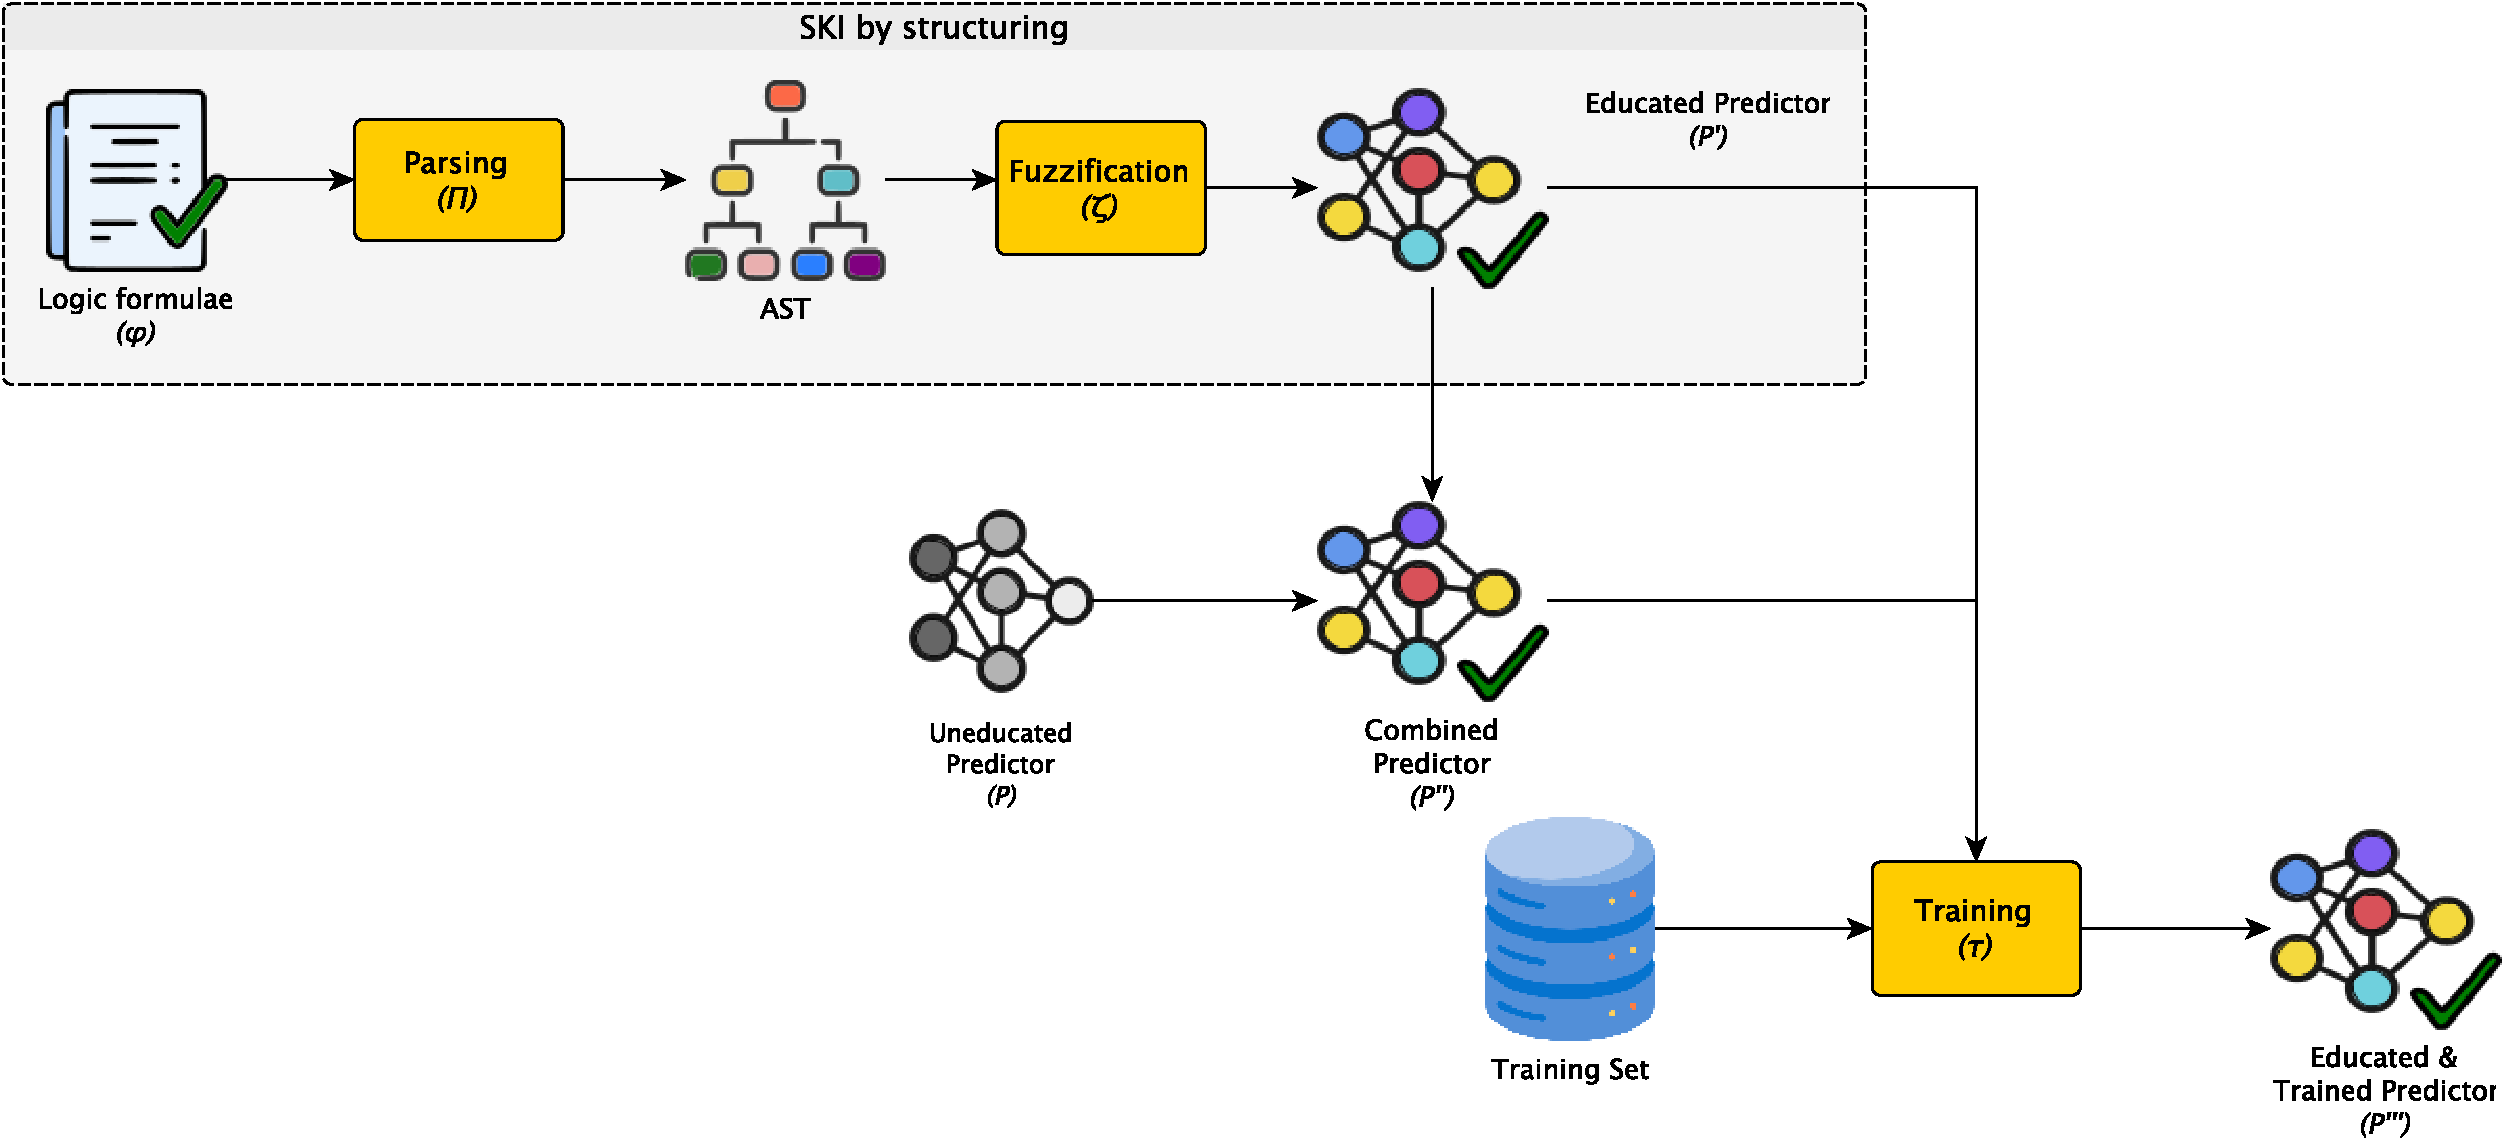
\includegraphics[width=.9\linewidth]{figures/workflow-structuring}
    \caption[SKI workflow of structuring strategy]{
        Workflow of the structuring strategy.
        %
        The symbolic knowledge is parsed and used to create a sub-symbolic predictor -- or part of it -- that mimics the symbolic knowledge.
        %
        The resulting predictor is then trained on data, if needed.
    }
    \label{fig:workflow-structuring}
\end{figure}
%
By predictor structuring, or simply structuring, we identify all those methods that use a part (or the whole) of a sub-symbolic predictor to \emph{mirror} the symbolic knowledge via its own internal structure.
%
A predictor is either created or extended to mimic the behavior of the symbolic knowledge.
%
For instance, when the predictors are \glspl{NN}, their internal structure is crafted to represent logic predicates via neurons, and logic connectives via synapses.
%
\Cref{fig:workflow-structuring} illustrates the workflow of the structuring strategy.
%
Usually, in the structuring strategy, the symbolic knowledge is in the form of logic formulas ($\phi$) (e.g., subsets of \gls{FOL}).
%
The formulas are then parsed into a syntactic structure (e.g., \gls{AST}).
%
At this point, a \emph{fuzzification} ($\zeta$) step is performed to convert the \emph{boolean} (also the term \emph{crisp} is used in the literature) -- because a logic predicate is either \emph{true} or \emph{false} -- symbolic knowledge into a \emph{fuzzy} interpretation of it, which is more suitable for sub-symbolic predictors.
%
This fuzzy interpretation is often \emph{continuous} and bounded to a predefined range, such as \([0, 1]\).
%
The property of continuity is a key requirement for training sub-symbolic structures via gradient descent (e.g., \glspl{NN} or part of them).
%
In practice, $\zeta$ is implemented as a mapping function that transforms logic operators into continuous functions (e.g., see \Cref{subsec:kill-fuzzifier,subsec:kins-fuzzifier}).
%
The result of the fuzzification process is an \emph{uneducated} predictor ($P$) that is then trained on the training set.
%
After the training, the predictor is now \emph{educated} ($P'$) and can be used to make predictions on the test set or in production.
%

\paragraph{Guided learning}\label{par:guided-learning}
%
\begin{figure}
    \centering
    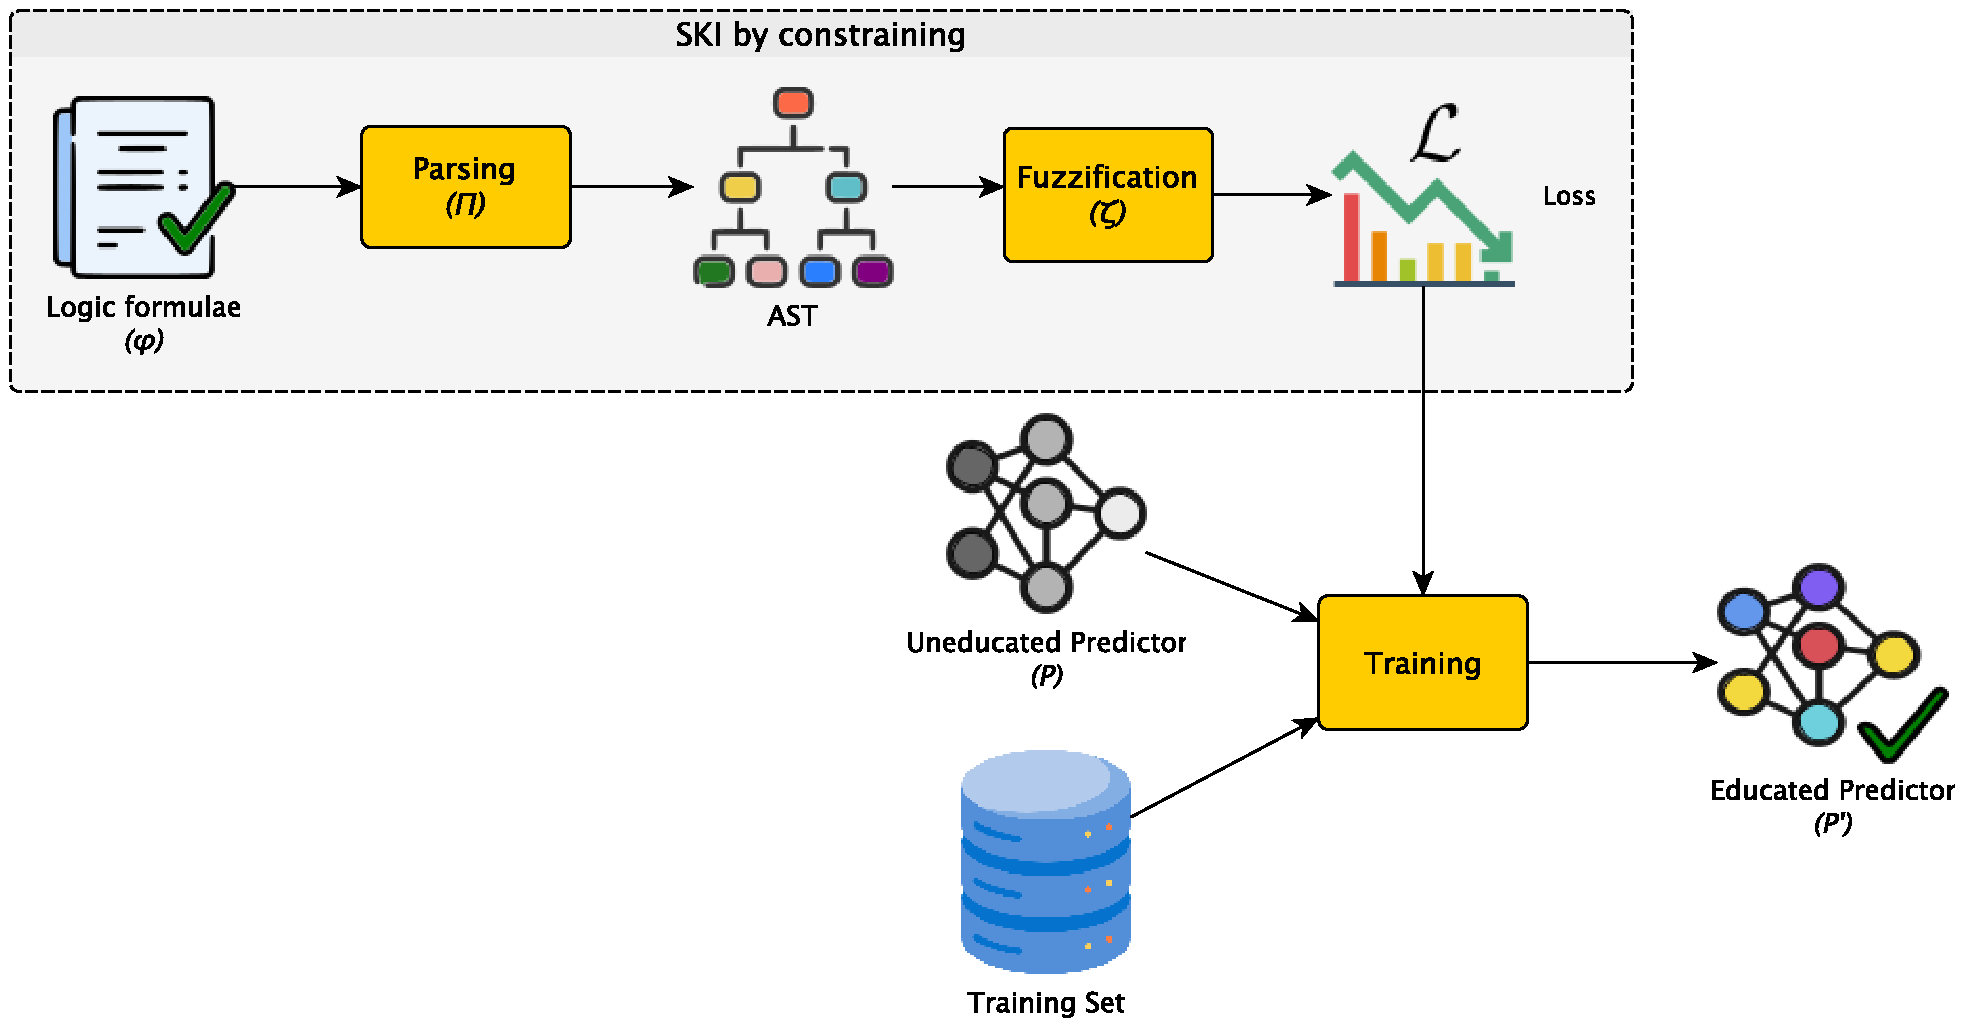
\includegraphics[width=.9\linewidth]{figures/workflow-constraining}
    \caption[SKI workflow of guided learning strategy]{
        \gls{SKI} workflow of the guided learning strategy.
        %
        The symbolic knowledge is used to guide the training of a sub-symbolic predictor, which is then trained on data.
    }
    \label{fig:workflow-learning}
\end{figure}
%
By guided learning, we refer to all those methods that affect the sub-symbolic predictor's training process by using the symbolic knowledge as a \emph{constraint}/\emph{guidance}.
%
Usually, \gls{SKI} algorithms based on this strategy target sub-symbolic predictors that can be trained with gradient descent, such as \glspl{NN}.
%
\Cref{fig:workflow-learning} illustrates the workflow of the guided learning strategy.
%
Like in the case of structuring, the symbolic knowledge is parsed and fuzzified.
%
Differently from structuring, the result of the fuzzification process is not a subcomponent of the predictor's architecture (e.g., neurons, connections), but rather a set of continuous numeric functions.
%
Conceptually, these functions represent the degree of violation of the symbolic knowledge by the predictor's predictions.
%
The higher the degree of violation, the higher the value of the function.
%
The symbolic-derived functions are then included in the loss function of the predictor, which is then trained on the training set.
%
The combination between the ``classical'' loss function (e.g., cross-entropy, mean squared error, etc.) and the symbolic-derived functions can be done in many ways, but it is usually done via a weighted sum.


\paragraph{Embedding}\label{par:ski-embedding}
%
\begin{figure}
    \centering
    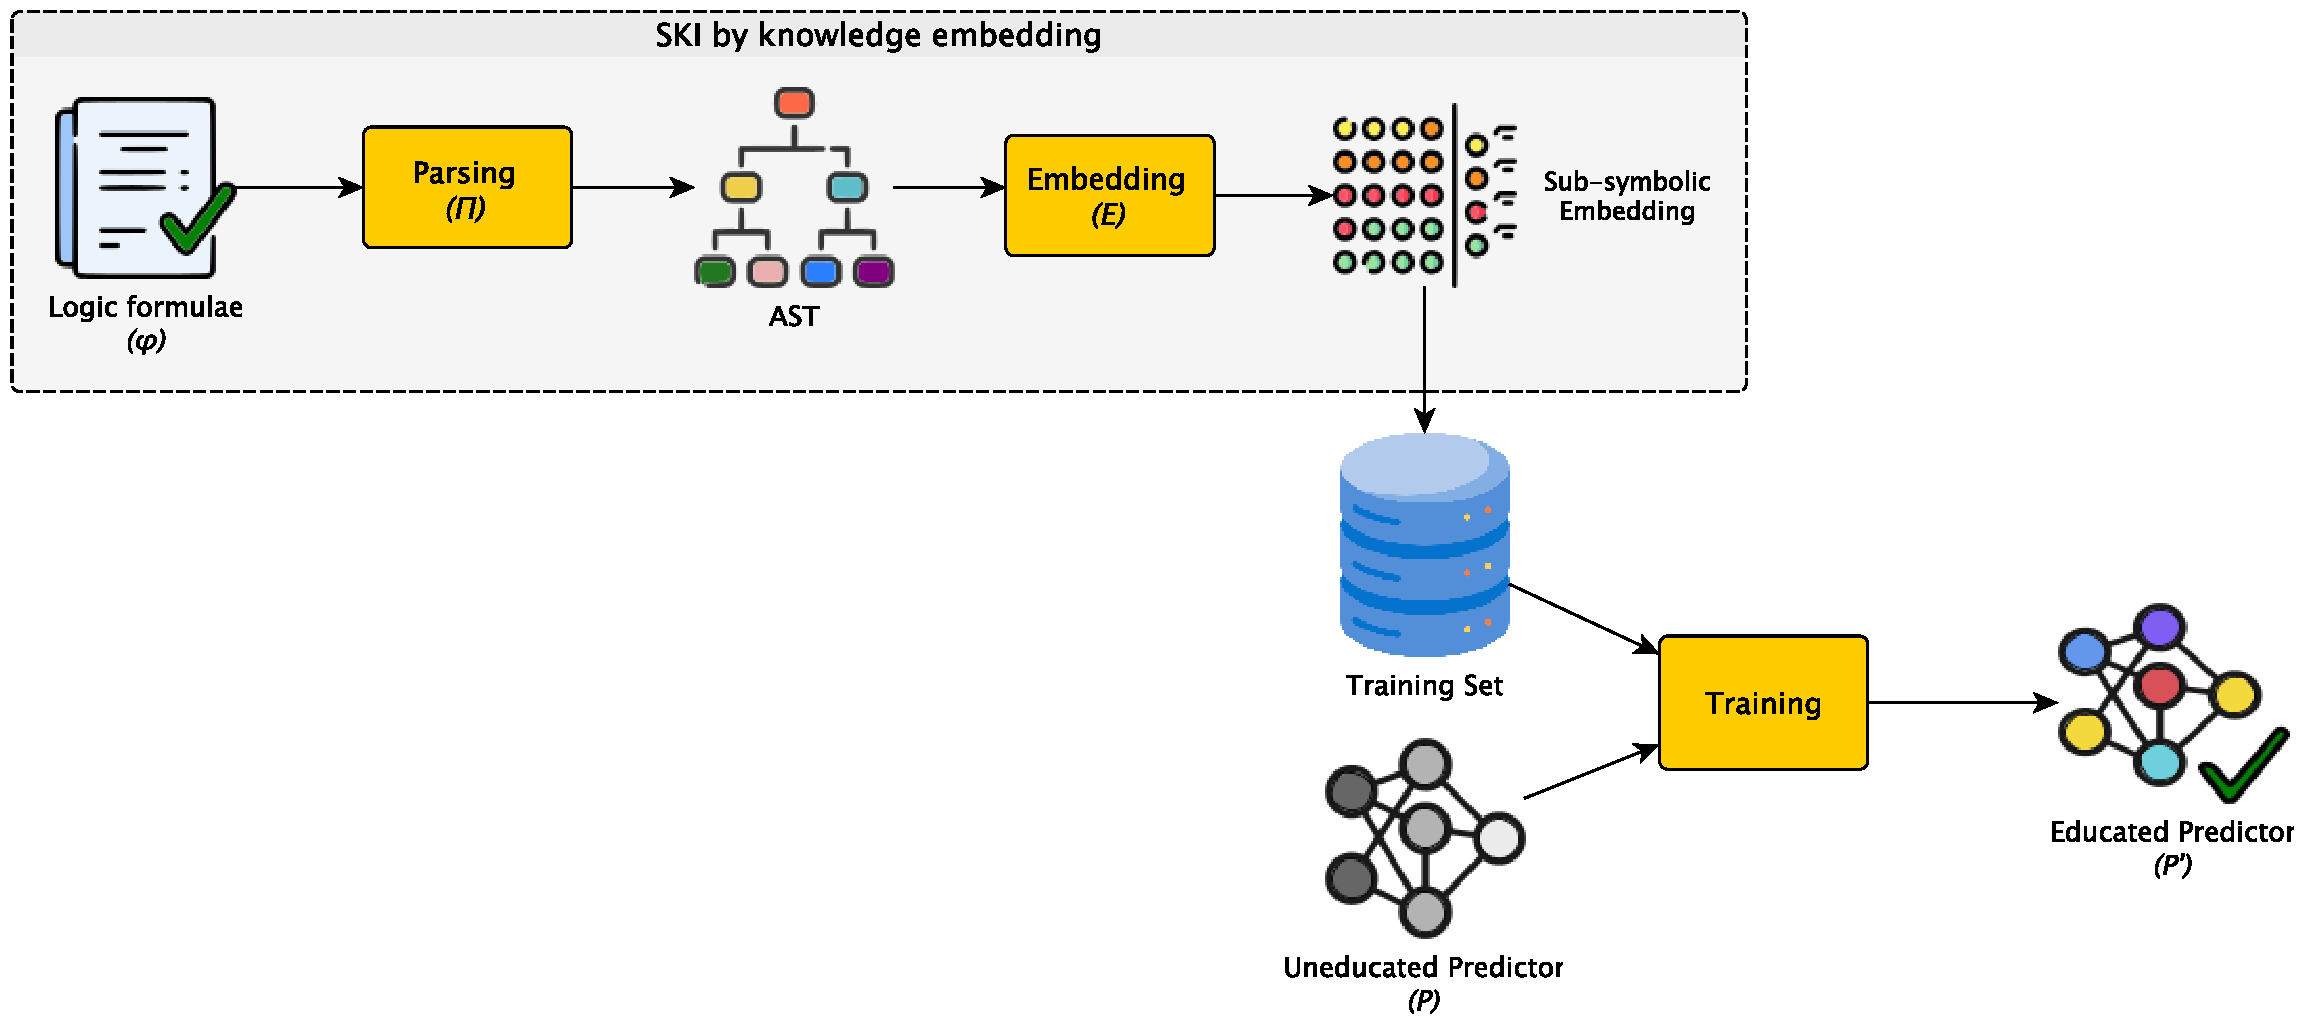
\includegraphics[width=.9\linewidth]{figures/workflow-embedding}
    \caption[SKI workflow of embedding strategy]{
        \gls{SKI} workflow of the embedding strategy.
        %
        The symbolic knowledge is parsed and embedded into a sub-symbolic predictor, which is then trained on data.
    }
    \label{fig:workflow-embedding}
\end{figure}
%
In the embedding strategy, the symbolic knowledge is converted -- i.e., \emph{embedded}-- into numeric-array representations.
%
\Cref{fig:workflow-embedding} illustrates the workflow of the embedding strategy.
%
The output of the fuzzification process is a set of numeric arrays (e.g., vectors, matrices, and tensors) that represent the symbolic knowledge.
%
These arrays are then provided as input to the sub-symbolic predictor.
%
This is the common strategy exploited by the \gls{KG}~\cite{DBLP:conf/ijcai/LambGGPAV20} embedding community as well as by \glspl{GNN}~\cite{DBLP:journals/tkde/WangMWG17}.


\subsection[Limitations and challenges of SKI]{Limitations and challenges of \Gls{SKI}}\label{subsec:limitations-and-challenges-of-ski}
%
Despite the numerous advantages of \gls{SKI}, there are several limitations and challenges that need to be addressed.
%
Here, we elicit the most common and relevant limitations and challenges of \gls{SKI} that we encountered in the literature:
%
\begin{itemize}
    %
    \item \textbf{Lack of generality}, many \gls{SKI} methods are tailored to domain-specific tasks.
    %
    Often, even if they are presented as general-purpose, their implementation is not and it requires significant effort to adapt them to different tasks or domains;
    %
    \item \textbf{Lack of reproducibility}, the experiments presented -- if any -- in the papers are often not reproducible.
    %
    This happens because the authors do not provide enough details about the implementation of the method (e.g., they do not mention the value of some key hyperparameters), or they do not share the code and data used in the experiments.
    %
    Only 49 out of 117 surveyed methods provide public code base for the experiments\footnote{\label{foot:supplementary}see Table B of the supplementary material of~\cite{DBLP:journals/csur/CiattoSAMO24}};
    %
    \item \textbf{Lack of availability}, the vast majority of \gls{SKI} methods is not available as open-source software.
    %
    Only 11 out of 117 surveyed methods provide a public library for the method$^{\ref{foot:supplementary}}$.
    %
    Authors usually do not mention any code base in their papers, and if they do, the code can lack the necessary dependencies, lack documentation, or it could have been removed from public repositories;
    %
    \item \textbf{Limits of the symbolic knowledge}, despite the variety of symbolic knowledge that can be injected (see \Cref{fig:pie-ski-logic}), there are still many limitations.
    %
    Indeed, the claimed expressiveness of the logic formalism supported by a method is often not fully exploited in practice.
    %
    In particular, \gls{FOL} allows for the representation of recursive terms, but most \gls{SKI} methods do not support them because of the target predictors.
    %
    Target predictors are almost always \glspl{NN}, which cannot support recursion in their architecture---modern \glspl{NN} are \glspl{DAG}.
    %
\end{itemize}

\section[Symbolic knowledge extraction]{\Glsentrylong{SKE}}\label{sec:ske}
%
\gls{SKE} is the process of extracting symbolic knowledge from sub-symbolic predictors.
%
Here, we provide the broad definition of \gls{SKE} that we adopt in this thesis:
%
\begin{definition}[\gls{SKE}]
    \label{def:ske}
    any \textbf{algorithmic} procedure accepting \textbf{trained} sub-symbolic predictors as input and producing \textbf{symbolic} knowledge as output so that the extracted knowledge reflects the behavior of the predictor with high \textbf{fidelity}~\cite{DBLP:journals/csur/CiattoSAMO24}.
\end{definition}
%
Once again, the definition is broad because the amount of contributions in the literature is vast and varied, they often use different terminologies and come from different communities.
%
\Gls{SKE} is conceptualized as a class of algorithms, which are finite-step procedures defined by their inputs and outputs.

The input to \gls{SKE} procedures must be trained \glspl{ML} predictors.
%
There are no restrictions on the type of predictor, meaning that \gls{SKE} methods can, in principle, be applied to any predictor family.
%
However, this requirement implies that the predictor must have already undergone training and achieved satisfactory performance for its intended task.
%
Thus, within an \gls{ML} workflow, \gls{SKE} is performed after the training and validation phases are complete.

The output of \gls{SKE} procedures is symbolic knowledge, which is broadly defined as human-intelligible information.
%
This can include logic formulas, decision trees, or even plain human-readable text.
%
For an algorithm to qualify as a valid \gls{SKE} procedure, the extracted knowledge must closely reflect the behavior of the original predictor within the domain it was trained for.
%
This fidelity is typically measured using a fidelity score, which evaluates how well the extracted knowledge replicates the predictor's behavior for the given task and domain.

The extracted knowledge should ideally function as a predictor itself, allowing it to be queried in the same way as the original predictor.
%
For example, if the original predictor is an image classifier, the extracted knowledge should enable an intelligent agent to classify similar images and produce equivalent results.
%
This agent could be either computational (e.g., a software program) or human, depending on whether the extracted knowledge is machine or human interpretable.
%
The use of logic-based knowledge as the target of \gls{SKE} is particularly advantageous, as it supports both machine and human interpretability.


\subsection{Motivations and goals}\label{subsec:ske-motivations-and-goals}
%
\Gls{SKE} serves multiple purposes, including:
%
\begin{inlinelist}
    %
    \item \label{itm:inspection} the inspection of the internal operations of opaque predictors, which are otherwise treated as black boxes,
    %
    \item \label{itm:automation} the automation and acceleration of the process of acquiring symbolic knowledge, eliminating the need for manually crafting \glspl{KB},
    %
    \item \label{itm:xai} providing valuable capabilities within the scope of \gls{XAI} to analyze black-box predictors.
\end{inlinelist}

\Cref{itm:inspection} is particularly important for understanding the behavior of opaque predictors.
%
By inspecting their internal operations, \gls{SKE} allows researchers and practitioners to identify patterns in mispredicted inputs or even detect correctly predicted patterns that rely on unethical or biased decision processes.
%
This capability is crucial for ensuring the ethical and transparent use of \gls{ML} systems, especially in sensitive domains such as healthcare or finance.

\Cref{itm:automation} highlights another key advantage of \gls{SKE}: the ability to automate the extraction of symbolic knowledge.
%
This eliminates the labor-intensive process of manually crafting \glspl{KB}, which often requires significant domain expertise and time.
%
By automating this process, \gls{SKE} not only accelerates knowledge acquisition but also enables the reuse of extracted knowledge across different tasks or systems, provided the knowledge is represented in a compatible format.

Finally, \Cref{itm:xai} emphasizes the role of \gls{SKE} in \gls{XAI}.
%
The extracted knowledge can be used to construct explanations for the behavior of black-box predictors, making their decision-making processes more interpretable.
%
In some cases, this knowledge may even serve as an interpretable surrogate model, replacing the original predictor if it achieves a high fidelity score~\cite{DBLP:conf/atal/CiattoCSO20}.
%
Additionally, \gls{SKE} enables the comparison of multiple black-box predictors performing the same task, highlighting their differences and commonalities.
%
It also facilitates the merging of knowledge extracted from various predictors, even if they belong to different families, as long as the same representation format is used~\cite{DBLP:conf/aiia/CiattoCOC19}.


\subsection{What to extract}\label{subsec:what-to-extract}
%
\begin{figure}
    \centering
    \includegraphics[width=.6\linewidth]{figures/ske-rule-shape}
    \caption[Venn diagram categorising SKE methods]{
        %
        Venn diagram categorising \gls{SKE} methods w.r.t.\ the \emph{shape} of the extracted symbolic knowledge: rule lists (L), decision trees (DT), decision tables (TA), or knowledge graphs (KG).
        %
        The image is taken from~\cite{DBLP:journals/csur/CiattoSAMO24} and it refers to 132 surveyed \gls{SKE} methods.
    }
    \label{fig:pie-ski-shape}
\end{figure}
%
\begin{figure}
    \centering
    \includegraphics[width=.6\linewidth]{figures/ske-rule-format}
    \caption[Pie chart categorising SKE methods]{
        %
        Pie chart categorising \gls{SKE} methods w.r.t.\ the semantic \emph{expressiveness} of the extracted symbolic knowledge: propositional rules (P), fuzzy rules (F), oblique rules (O), m-of-n rules (MN), or triplets (T).
        %
        The image is taken from~\cite{DBLP:journals/csur/CiattoSAMO24} and it refers to 132 surveyed \gls{SKE} methods.
    }
    \label{fig:pie-ski-expressiveness}
\end{figure}

What kind of symbolic knowledge can be extracted?
%
Symbolic knowledge extracted from \glspl{ML} predictor should ideally mimic the behavior of the predictor itself.
%
For supervised \gls{ML}, this means that the extracted knowledge should represent a function mapping input features to output features, such as classes in classification tasks.
%
These functions can be expressed in symbolic formats, which vary in both syntax and semantics.

\paragraph{Shape of the extracted knowledge}
%
From a syntactic perspective, the shape of the extracted symbolic knowledge is crucial for its interpretability.
%
The most common formats include decision rules and decision trees, as they are widely recognized for their human-comprehensibility.
%
Other formats, such as decision tables and knowledge graphs, are also used, though less frequently.
%
Regardless of the format, the extracted knowledge typically uses symbols to represent the same input and output features as the original \gls{ML} predictor.

We identify four primary syntactic shapes for extracted symbolic knowledge:
%
\begin{itemize}
    \item \textbf{Lists of rules:} Sequences of logic rules presented in a predefined order.
    %
    \item \textbf{Decision trees:} Hierarchical structures where each node represents a decision rule (see \Cref{subsubsec:decision-trees}).
    %
    \item \textbf{Decision tables:} Tabular representations specifying conclusions for different sets of conditions.
    %
    These can be exhaustive, listing all possible combinations, or incomplete, covering only a subset of cases.
    %
    Each row (or column) corresponds to a rule, with cells indicating variable values.
    %
    An example is provided in the supplementary material.
    %
    \item \textbf{Knowledge graphs:} Graph-based representations of entities and their relationships (see \Cref{subsubsec:ontologies-and-kg}).
\end{itemize}

\Cref{fig:pie-ski-shape} illustrates the distribution of these shapes across surveyed \gls{SKE} methods.
%
Rule lists are the most prevalent, likely due to their simplicity and algorithmic tractability.

\paragraph{Expressiveness of the extracted knowledge}
%
From a semantic perspective, the expressiveness of the extracted symbolic knowledge depends on the logical constructs it employs.
%
Statements may include predicates, relations, logic connectives, and arithmetic comparators, which determine what can be expressed.
%
We categorize the semantic formats of extracted symbolic knowledge as follows:
%
\begin{itemize}
    \item \textbf{Propositional rules:} Statements involving Boolean input/output features connected by logic operators such as negation, conjunction, and disjunction.
    %
    Arithmetic comparisons between continuous features and constants are also included in this category.
    %
    \item \textbf{Fuzzy rules:} Extensions of propositional rules where truth values range continuously between 0 and 1.
    %
    \item \textbf{Oblique rules:} Rules with conditions expressed as inequalities involving linear combinations of input variables, allowing comparisons between features.
    %
    \item \textbf{m-of-n rules:} Rules that are true if at least \(m\) out of \(n\) conditions are satisfied.
    %
    These are a concise way of representing disjunctions of conjunctions.
    %
    \item \textbf{Triplets:} Representations commonly used in knowledge graphs, consisting of subject-predicate-object triples (see \Cref{subsubsec:ontologies-and-kg}).
\end{itemize}

\Cref{fig:pie-ski-expressiveness} summarizes the occurrence of these semantic formats in surveyed \gls{SKE} methods.
%
Propositional rules dominate due to their simplicity and tractability.
%
They allow a divide-and-conquer approach, focusing on one input feature at a time, which simplifies the extraction process.


\subsection{Where to extract}\label{subsec:where-to-extract}
%
\begin{figure}
    \centering
    \includegraphics[width=.6\linewidth]{figures/ske-translucency}
    \caption[Venn diagram categorising SKE methods]{
        %
        Venn diagram categorising \gls{SKE} methods w.r.t.\ the \emph{translucency} of the algorithm: decompositional (D) or pedagogical (P).
        %
        For decompositional methods, we report the target predictor type: ANN<n> = artificial \gls{NN} (possibly having exactly <n> layers), CNN = convolutional \gls{NN}, GNN = graph \gls{NN}, FNN = fuzzy \gls{NN}, SVM = support vector machines, DTE = decision tree ensembles, LC = linear classifiers.
        %
        The image is taken from~\cite{DBLP:journals/csur/CiattoSAMO24} and it refers to 132 surveyed \gls{SKE} methods.
    }
    \label{fig:pie-ske-translucency}
\end{figure}
%
The sort of \gls{ML} predictors from which symbolic knowledge can be extracted is strongly related to the \emph{translucency} of the \gls{SKE} algorithms.
%
The translucency of a \gls{SKE} algorithm refers to its ability to access the internal structure of the predictor, such as its parameters, weights, and architecture.
%
So, in other words, the question of where to extract symbolic knowledge is related to the question of how \gls{SKE} algorithms work.
%
There are two ways for \gls{SKE} methods to deal with sub-symbolic predictors:
%
\begin{itemize}
    \item \textbf{Decompositional} $\rightarrow$ if the method needs to inspect -- even partially -- the internal structure of the predictor, such as its parameters, weights, and architecture;
    %
    \item \textbf{Pedagogical} $\rightarrow$ if the method does not need to inspect the internal structure of the predictor, but rather it can treat it as a black box and it relies on the input/output behavior of the predictor.
\end{itemize}

The different nature of decompositional \gls{SKE} methods is detailed in \Cref{fig:pie-ske-translucency}.
%
We observe that for what concern decompositional methods, the vast majority of them are designed to work with \gls{NN} of various types and different number of hidden layers.
%
Also \glspl{SVM} and \glspl{DTE} are targeted by some decompositional methods.
%
Around 43\% of the surveyed methods are pedagogical, meaning that these methods can work with virtually any type of sub-symbolic predictor, as long as it can be queried for input/output pairs.
%
Therefore, in general \gls{SKE} methods can be applied to any type of predictor, but for the decompositional ones, \glspl{NN} are definitely the most targeted type.


\subsection{How to extract}\label{subsec:how-to-extract}
%
The way \gls{SKE} methods extract symbolic knowledge highly depends on the translucency of the method itself.
%
Pedagogical methods treat the underlying predictor as an oracle to be queries for predictions the symbolic knowledge should mimic.
%
\note{TODO: add citations}
%
In most of these cases, the \gls{SKE} method exploits a \emph{surrogate} model, which is a simpler, more interpretable model that approximates the behavior of the original predictor.
%
This model can be used as the final output of the \gls{SKE} process if it is already in a symbolic or interpretable (e.g., a linear model) format, or it can be further processed to extract symbolic knowledge.
%
Decompositional methods, on the other hand, require access to the internal structure of the predictor and each method has its own way of extracting symbolic knowledge.
%
\note{TODO: does it make sense to talk about this here?}
%
Another important aspect of \gls{SKE} methods when it comes to how symbolic knowledge is extracted is the \emph{granularity} of the extraction.

\paragraph{Local explanations}\label{par:local-explanations}
%
\begin{figure}
    \centering
    \includegraphics[width=.6\linewidth]{figures/local-explanation}
    \caption[Local explanations]{
        %
        Simple example to of how a local explanation can be provided for a specific input.
        %
        The sub-symbolic model's decision function $f$ is represented by the blue and pink background, which cannot be approximated well by a linear model.
        %
        The bold red cross is the instance being explained.
        %
        A \gls{SKE} method can sample inctances, get prediction using $f$, and weights them by the proximity to the instance being explained (the bigger the cross/circle, the closer to the instance).
        %
        The dashed line is the trained interpretable model that is locally faithful to the sub-symbolic model.
        %
        The image is taken from~\cite{DBLP:conf/kdd/Ribeiro0G16}.
    }
    \label{fig:local-explanations}
\end{figure}
%
When the interest in the extracted symbolic knowledge is focused on a specific input, i.e., we want to know why a predictor produced a particular outcome, the \gls{SKE} method is said to produce \emph{local explanations}.
%
A local explanation is symbolic knowledge that explains only the behavior of the predictor for a specific input.
%
The knowledge is not necessary encoded into logic rules, it can be provided for instance through \emph{feature importance} scores, which indicate the relevance of each input feature for the prediction~\cite{DBLP:conf/kdd/Ribeiro0G16}.
%
\Cref{fig:local-explanations} illustrates a simple example of how a local explanation can be provided for a specific input using a pedagogical \gls{SKE} method.


\paragraph{Global explanations}\label{par:global-explanations}
%
Conversely, when the interest is in understanding the overall behavior of the predictor, we say that the \gls{SKE} method produces \emph{global explanations}.
%
Global explanations aim to capture the general patterns and rules that govern the predictor's behavior across all inputs, rather than focusing on individual instances.
%
For example, this can be done by training a surrogate model -- if we want to use a pedagogical \gls{SKE} method -- using for instance the training set used to train the predictor.
%
However, instead of using the labels of the training set, the surrogate model is trained using the predictions of the original predictor.


\subsection[Limitations and challenges of SKE]{Limitations and challenges of \Gls{SKE}}\label{subsec:limitations-and-challenges-of-ske}
\note{TODO}
%%! Author = matteomagnini
%! Date = 05/03/25

%----------------------------------------------------------------------------------------
\chapter{Large Language Models}
\label{ch:llm}
\mtcaddchapter
\minitoc
%----------------------------------------------------------------------------------------

\section{Architectures}\label{sec:llm-architectures}

\subsection{Transformer}\label{subsec:transformer}

\subsection{Attention}\label{subsec:attention}

\section{Fine-tuning}\label{sec:llm-fine-tuning}

\section{\Glsentrylong{RAG}}\label{sec:rag}

\subsection{Embedding}\label{subsec:rag-embedding}

\subsection{Retrieval}\label{subsec:retrieval}

\section{Limitations and challenges}\label{sec:limitations-and-challenges}

\subsection{Resources}\label{subsec:resources}

\subsection{Data and privacy}\label{subsec:data-and-privacy}

\subsection{Hallucinations}\label{subsec:hallucinations}

\subsection{Stochastic parrot or something more?}\label{subsec:stochastic-parrot-or-something-more}
%\printbibliography[title=References,heading=bibintoc]
%\end{refsection}

%----------------------------------------------------------------------------------------
%-------------------------------------- PART II -----------------------------------------
%----------------------------------------------------------------------------------------

\part{Methods, Metrics and Platform for SKI \& SKE}
\label{part:engineering-of-ski-ske}

%\begin{refsection}
\input{chapters/chapter_4_ski_methods}
%! Author = matteomagnini
%! Date = 05/03/25

%----------------------------------------------------------------------------------------
\chapter[Platform for symbolic knowledge injection]{\Glsentrylong{PSyKI}}
\label{ch:psyki}

\begin{flushright}
\begin{minipage}{0.5\textwidth}
    How to \emph{facilitate} the engineering of \gls{SKI} methods?

    How to measure the \emph{\glsentrylong{QoS}} of \gls{SKI} methods?

    -- \textbf{\Cref{itm:rq0,itm:rq2,itm:rq3}}
\end{minipage}
\end{flushright}

\minitoc
%----------------------------------------------------------------------------------------

In this chapter, we present the \Gls{PSyKI} platform, which is a framework for \gls{SKI} methods.
%
\Gls{PSyKI} provides a unified way to implement \gls{SKI} methods, aiming to facilitate the development and comparison of different approaches.
%
It also provides a set of tools to evaluate the performance of \gls{SKI} methods, including metrics for measuring the quality of the injected knowledge and the performance of the resulting models.
%
In \Cref{sec:psyki}, we present the work ``\emph{On the Design of PSyKI: A Platform for Symbolic Knowledge Injection into Sub-symbolic Predictors}''~\cite{DBLP:conf/atal/MagniniCO22}, which describes the design and implementation of \gls{PSyKI}.
%
Then, in \Cref{sec:ski-meets-intelligent-agents,sec:empirical-study-on-the-robustness-of-ski-methods}, we present respectively two works that study the quality of service of \gls{SKI} methods:
%
in \Cref{sec:ski-meets-intelligent-agents} the paper ``\emph{Symbolic Knowledge Injection Meets Intelligent Agents}''~\cite{DBLP:journals/aamas/AgiolloRMCO23},
%
which introduces metrics for evaluating the performance of \gls{SKI} methods in the context of intelligent agents,
%
and in \Cref{sec:empirical-study-on-the-robustness-of-ski-methods} the paper ``\emph{An Empirical Study on the Robustness of Symbolic Knowledge Injection Techniques Against Data Degradation}''~\cite{DBLP:conf/woa/RafanelliMACO24},
%
which studies the robustness of \gls{SKI} methods against data degradation.


\section{One platform to bring them all}\label{sec:psyki}
%
\Gls{PSyKI} is a (Python) platform for the development and evaluation of \gls{SKI} methods.
%
It is designed to provide a unified framework for implementing \gls{SKI} methods, allowing researchers and practitioners to easily develop, test, and compare different approaches.
%
In the following, we present a summary of the work ``\emph{On the Design of PSyKI: A Platform for Symbolic Knowledge Injection into Sub-symbolic Predictors}''~\cite{DBLP:conf/atal/MagniniCO22}, presented at the 4th international workshop on \gls{EXTRAAMAS}, 2022\footnote{\url{https://extraamas.ehealth.hevs.ch/archive.html}}.
%
The platform is meant to be an open-source library that can be easily extended with new \gls{SKI} methods and evaluation metrics.
%
The library is public available on GitLab and PyPi\footnote{\url{https://gitlab.com/psykei/psyki-python} and \url{https://pypi.org/project/psyki/}}.


\subsection{Motivations}\label{subsec:psyki-motivations}
%
This work is motivated by the need to address the common challenges that affect \gls{SKI} methods (see \Cref{subsec:limitations-and-challenges-of-ski}).
%
In particular, we want to address the following points:
%
\begin{inlinelist}
    \item \emph{lack of generality}, by providing the proper tools to automatically translate symbolic knowledge of arbitrary domains into a format suitable for injection into sub-symbolic predictors,
    %
    \item \emph{lack of reproducibility}, by providing a unified framework for implementing \gls{SKI} methods, allowing researchers to easily develop, test, and compare different approaches, and
    %
    \item \emph{lack of availability}, by encouraging the development of reusable software libraries for \gls{SKI} methods.
    %
\end{inlinelist}
%
Concerning the last point mentioned in \Cref{subsec:limitations-and-challenges-of-ski}, we identified in the logic language of stratified Datalog with negation a suitable candidate for the symbolic knowledge representation.
%
It is expressive enough to represent a wide range of symbolic knowledge, while being simple enough to be easily translated into a format suitable for injection into sub-symbolic predictors.

This work differs from previous recent efforts in the area of \gls{SKI} software -- e.g., \gls{LTN}~\cite{BadreddineGSS22} and DeepProbLog~\cite{ski-deepproblog-robin-2021} -- because our platform is not designed to support just one injection method, but it is meant to be an extendable library of \gls{SKI} methods.
%
Moreover, \gls{PSyKI} provides a set of tools to evaluate the performance of \gls{SKI} methods, including metrics for measuring the quality of the injected knowledge and the performance of the resulting models.
%
Arguably, the most similar work -- \emph{but it came one year after the publication of \gls{PSyKI}} -- is Scallop~\cite{DBLP:journals/pacmpl/LiHN23}, a DataLog-based framework that supports differentiable logical and relational reasoning.


\subsection{Design}\label{subsec:design-and-implementation}
%
\begin{figure}
    \centering
    \includegraphics[width=\textwidth]{figures/knowledge-workflow-psyki}
    \caption[Symbolic knowledge transformation in PSyKI]{
        General workflow of symbolic knowledge transformation in \Gls{PSyKI}.
        The symbolic knowledge ($\phi$), typically expressed as logical formulas, is first parsed into a visitable form ($\phi'$), and then fuzzified into a machine-injectable representation ($\phi''$).
    }
    \label{fig:knowledge-workflow-psyki}
\end{figure}
%
All symbolic knowledge injection (\gls{SKI}) methods implemented in \gls{PSyKI} share a common transformation pipeline, illustrated in \Cref{fig:knowledge-workflow-psyki}.
%
Symbolic knowledge \(\phi\) cannot usually be injected directly into a sub-symbolic predictor.
%
Instead, it undergoes a two-step transformation:
%
\begin{inlinelist}
    %
    \item \emph{Parsing} (\(\Pi\)): the knowledge is converted into a visitable data structure, such as an \gls{AST} in the case of logic formulas, resulting in \(\phi'\);
    %
    \item \emph{Fuzzification} (\(\zeta\)): the parsed representation is transformed into a sub-symbolic form \(\phi''\), suitable for injection.
    %
\end{inlinelist}
%
Fuzzification plays a key role in bridging the symbolic and sub-symbolic domains.
%
It translates crisp Boolean logic into a form compatible with sub-symbolic models, often by relaxing discrete truth values into continuous-valued functions or generating neural components such as layers or entire \glspl{NN}.

\begin{figure}
    \centering
    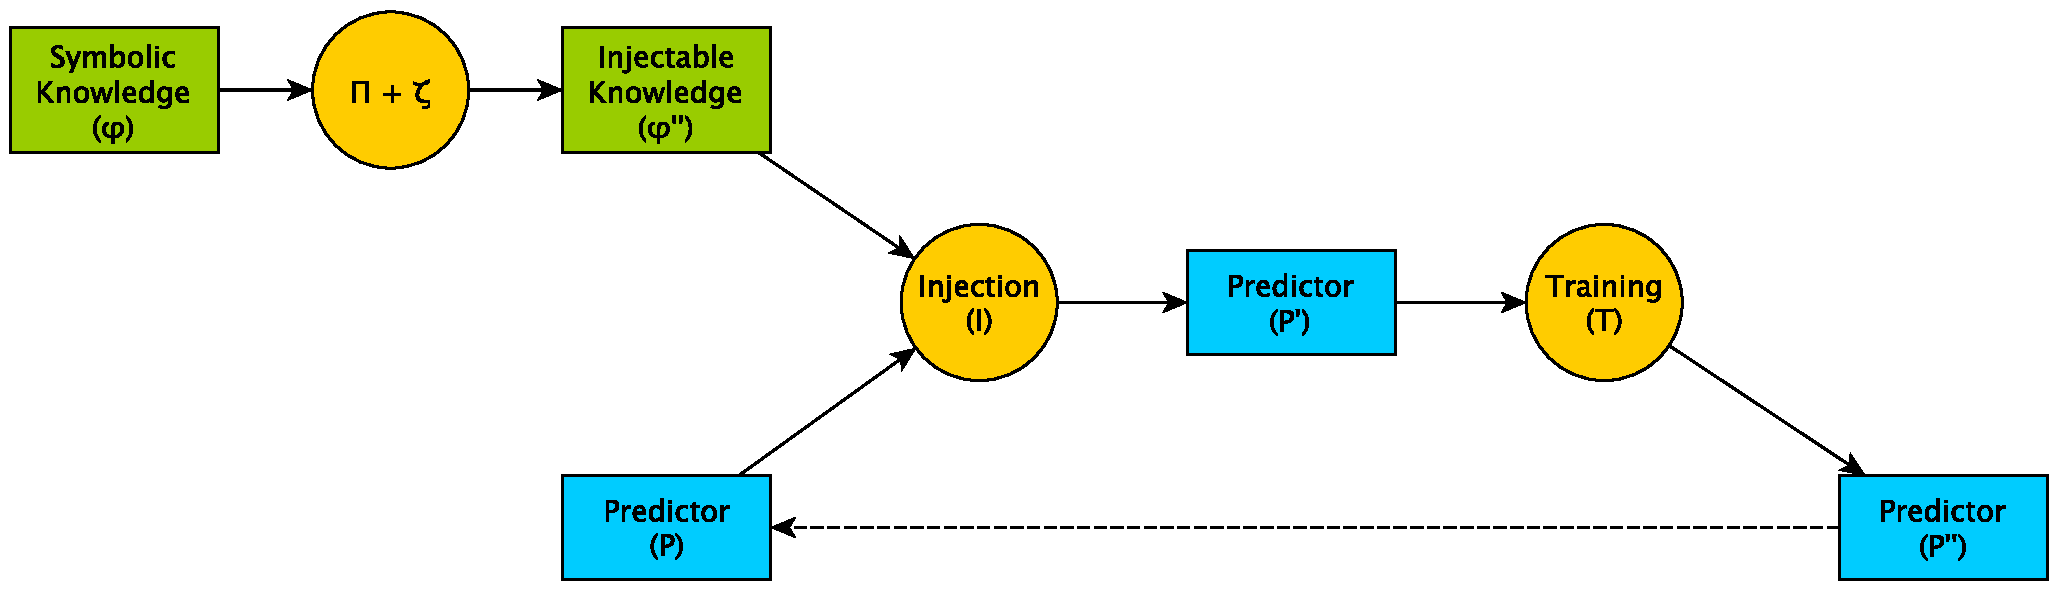
\includegraphics[width=\textwidth]{figures/psyki-workflow}
    \caption[General workflow of PSyKI]{
        Complete workflow of structuring and guided learning \gls{SKI} methods in \Gls{PSyKI}.
        The symbolic knowledge is transformed and injected into the sub-symbolic predictor, which is then trained on data.
    }
    \label{fig:psyki-workflow}
\end{figure}
%
\Cref{fig:psyki-workflow} shows the overall injection process in \gls{PSyKI}, including both the transformation of the symbolic knowledge and its integration into the learning system.
%
After the transformation phase, the different \gls{SKI} methods diverge:
%
\begin{inlinelist}
    %
    \item \emph{Structuring} and \emph{guided learning} inject \(\phi''\) directly into the architecture or training process of the predictor;
    %
    \item \emph{Embedding}-based methods use symbolic knowledge to enrich or generate the input data, so they are not directly represented in \Cref{fig:psyki-workflow}.
    %
\end{inlinelist}

\Gls{PSyKI} supports all three approaches, although it is primarily designed for \emph{structuring} and \emph{guided learning}, where the injection occurs directly into the predictor.
%
In general, \gls{SKI} algorithms operate on a predictor \(P\) and symbolic knowledge \(\phi\), producing a new predictor \(P'\) as output.
%
This modified predictor is then trained on data, resulting in a final model \(P''\), which can be reused in further iterations with different knowledge or injection strategies.


\paragraph{Architecture}\label{par:architecture}
%
\begin{figure}
    \centering
    \includegraphics[width=\textwidth]{figures/class-diagram}
    \caption[Class diagram of PSyKI]{
        Class diagram of \Gls{PSyKI}.
        %
        The main components are the \emph{Injector}, the \emph{Formula} and the \emph{Fuzzifier}.
        %
        The package \emph{logic.datalog} is an examplification showing two \emph{Injector} implementations and their relationships.
    }
    \label{fig:psyki-class-diagram}
\end{figure}
%
Essentially, \gls{PSyKI} is designed around the notion of injector.
%
An injector is any algorithm accepting a \gls{ML} predictor and prior symbolic knowledge -- predominantly logic formulas -- as input that produces a new predictor as output.
%
In order to properly perform injection, injectors may require additional information such as algorithm specific hyperparameters.


\gls{PSyKI} supports the processing of symbolic knowledge represented via logic formulas.
%
Based on the sort of logic, user can build an \gls{AST} for each formula.
%
The \gls{AST} can be inspected through a fuzzifier via pattern visitor to encode the symbolic knowledge to a sub-symbolic form (e.g. fuzzy logic functions, ad-hoc layers).
%
The resulting sub-symbolic object can finally be used by an injector to create a new predictor.
%
This process -- denoted with $\zeta$ \Cref{fig:psyki-workflow} -- is injector specific; instead, the same parser $\Pi$ can be used for logic formulas of the same sort independently of the injector.


The software is organized into well-separated packages to ensure easy extensibility towards new sort of logic and fuzzifiers---see \Cref{fig:psyki-class-diagram}
%
An \gls{AST} is a \emph{formula} object, and it can have different language specific elements w.r.t. the logic form that is covered.
%
Each formula implementation is self-contained inside a standalone package so that if a user wants to add a new logic form it is sufficient to add its implementation in a new package.
%
Similarly, a fuzzifier object that targets a specific logic form can be added inside the same package of the logic, there can be any number of fuzzifiers for a given logic.


\subsection{Implementation}\label{subsec:psyki-implementation}
%
\paragraph{Knowledge representation}\label{par:knowledge-representation}
%
\begin{figure}
    \centering
    \includegraphics[width=\textwidth]{figures/grammar}
    \caption[Class diagram for the representation of Datalog formulas]{
        A supported grammar of \Gls{PSyKI} for logic formulas.
        %
        The grammar is designed to represent Datalog formulas.
    }
    \label{fig:grammar}
\end{figure}
%
A crucial point in the \gls{SKI} workflow is the embedding of knowledge from symbolic into sub-symbolic form.
%
Ideally, there is no constraint on the formalism used to represent the prior knowledge (e.g., logic formulas, knowledge graph).
%
The most common knowledge representation form that \gls{SKI} algorithms claim to support is \gls{FOL} or one of its subsets.
%
However, there are characteristics of \gls{FOL} that are not ideal for some predictors.
%
Recursion and function symbols -- that allow recursive structures -- cannot be easily integrated into a predictor that is acyclic -- i.e., no recursive -- by construction such as conventional \gls{NN} (virtually all \gls{NN}, with few exceptions like fibred \gls{NN}~\cite{DBLP:conf/flairs/BaderGH05}).
%
Conversely, in this work we consider one of the most general and expressive logic formalism that does not support recursion and function symbols: stratified Datalog with negation.


Stratified Datalog with negation has been already described in detail in \Cref{subsec:ski-stratified-datalog-with-negation}.
%
To support injection into a particular predictor, we further assume the input knowledge base defines at least one outer relation -- say output or class -- involving as many variables as the input and output features the predictor has been trained upon.
%
Such a relation may be defined via one or more clauses, and each clause may leverage on other predicates in their bodies.
%
In turn, each predicate may be defined through one or more clause.
%
In that case, since we rely on stratified Datalog, we require input knowledge to not include any (directly or indirectly) recursive clause definition.


Once that the logic has been formalized, the implementation of a \emph{Formula} -- visitable data structure like an \gls{AST} -- is quite straightforward.
%
\Cref{fig:grammar} depicts the general API for representing logic formulas, as currently supported by \gls{PSyKI}.
%
To make \gls{PSyKI} able to parse bare text into actual logic formulas compliant to that API, we rely on well-established parser-generation facilities such as ANTLR~\cite{DBLP:journals/spe/ParrQ95}.
%
As further discussed below, the knowledge contained into a Formula object, can then be embedded in sub-symbolic form, via a fuzzifier, to be later injected into a predictor.


Later in the evolution of \gls{PSyKI} (i.e., from v. 0.2.1), we considered switching to a more established logic language for representing the symbolic knowledge: Prolog~\cite{DBLP:journals/tplp/KornerLBCDHMWDA22}.
%
In particular, we abandoned the manual parsing of logic formulas with ANTLR, and we rely on the tuProlog~\cite{DBLP:conf/padl/DentiOR01} framework.
%
We use the parser of tuProlog to parse the logic formulas, but \gls{PSyKI} does not support the full Prolog language because of the limitations of injecting into \gls{NN} mentioned in \Cref{subsec:limitations-and-challenges-of-ski} (i.e., we still support only stratified Datalog with negation).


\paragraph{Fuzzification}\label{par:fuzzification}
%
While logic formulas are commonly interpreted in a Boolean way -- i.e., they can be assigned with one truth value among true and false --, sub-symbolic predictors are more flexible-hence supporting formulas to hold up to some extent.
%
Switching from the former interpretation to the latter is, essentially, the purpose of fuzzifiers.
%
In practice, this implies converting a logic formula into a function of real numbers.
%
Along this line, fuzzification may be performed in (at least) two ways; real numbers may either represent
%
\begin{inlinelist}
    %
    \item a \emph{penalty} for the violation of a formula, or
    %
    \item the \emph{degree of truth} of that formula.
    %
\end{inlinelist}

To serve this purpose, one may rely on a multivalued interpretation of logic inspired to $\L$ukasiewicz's logic, where the value true is represented by 0 (resp. 1), while higher (resp. lower) values represent ``falsity''.
%
In particular, this approach may be useful to constrain a predictor during its training.
%
Examples of this fuzzification approach are \gls{KILL} (\Cref{subsec:kill-fuzzifier}) and \gls{KINS} (\Cref{subsec:kins-fuzzifier}).
%
\Cref{tab:kill-logic-formulae,tab:kins-logic-formulae} show the logic formulas encoding into real-valued functions for \gls{KILL} and \gls{KINS}, implementing \emph{penalty} and \emph{degree of truth} respectively.


\paragraph{Injection}\label{par:injection}
%
\lstinputlisting[
    basicstyle=\fontsize{8}{9.5}\ttfamily\selectfont,
    label=lst:psyki-injection,
    float,
    caption={General code snippet for the use of a \gls{SKI} method in the current version of \glsentryshort{PSyKI} (v. 0.4.3).},
    captionpos=b,
    language=Python,
]{listings/psyki-injection.py}
%
Knowledge injection is the central step in \gls{SKI}.
%
It is carried out by \emph{injectors}, i.e., objects wrapping a particular injection strategy.
%
Each injector is expected to accept one sub-symbolic predictors as input, other the logic formulas that should be injected into that predictor.
%
As part of its operation, the injector is in charge of producing a new predictor as output, of the same type as the one provided as input.
%
The new predictor is altered in such a way that it is consistent w.r.t. the provided logic formulas.


While the main architecture of \gls{PSyKI} has been maintained stable during the years, the implementation has been continuously improved.
%
The current version of \gls{PSyKI} (v. 0.4.3) is implemented in Python 3.9.13, with main dependencies being \texttt{tensorflow}, \texttt{2ppy}, \texttt{scikit-learn}, and \texttt{pandas}.
%
\Cref{lst:psyki-injection} shows a general code snippet for the use of a \gls{SKI} algorithm in \gls{PSyKI} (v. 0.4.3).


\section[QoS metrics for SKI methods]{\Gls{QoS} metrics for \gls{SKI} methods}\label{sec:ski-meets-intelligent-agents}
%
In this section and in the next one, we present two works that study the \gls{QoS} of \gls{SKI} methods.
%
\Gls{QoS} is a crucial aspect of any non-trivial systems, and it is particularly important for \gls{SKI} because the vast majority of the works in this field do not provide any evaluation but the performance of the resulting model.
%
Moreover, \gls{SKI} methods and the resulting educated models have many other dimensions that can be evaluated a part from the straight prediction performance.
%
The metrics introduced in these works have been implemented and integrated into \gls{PSyKI} from version 0.2.14 and later.


The work ``\emph{Symbolic Knowledge Injection Meets Intelligent Agents}''~\cite{DBLP:journals/aamas/AgiolloRMCO23}, published in the \emph{Autonomous Agents and Multi-Agent Systems} journal, presents a set of metrics for evaluating the performance of \gls{SKI} methods in the context of intelligent agents.
%
Here we present a summary of the work, including the motivations, the proposed metrics, and the evaluation of \gls{SKI} methods in terms of \gls{QoS}.


\subsection{Motivations}\label{subsec:ski-meets-intelligent-agents-motivations}
%
The current practice of assessing \gls{SKI} methods primarily focuses on measuring improvements in the predictive performance of an educated predictor \(\hat{N}\) over its uneducated counterpart \(N\).
%
However, predictive performance is not the only relevant benefit of \gls{SKI} that should be evaluated.

There are multiple aspects of \glspl{ML} predictors that can be influenced by \gls{SKI}, and for which specific metrics should be defined.
%
For instance, \gls{SKI} may impact the \emph{memory footprint}, \emph{latency}, \emph{data efficiency}, and \emph{energy consumption} of the predictors it is applied to.
%
Collectively, these properties contribute to what we refer to as the \emph{efficiency} of a predictor.

In this work, we consider the following efficiency properties:
%
\begin{properties}
    \item \textbf{Memory footprint}: the size of the predictor, typically measured in terms of the number of parameters or computational operations required.
    %
    \label{itm:memory-footprint}
    %
    \item \textbf{Latency}: the time required to perform a single inference.
    %
    \label{itm:latency}
    %
    \item \textbf{Data efficiency}: the amount of data required to train the predictor to achieve a certain level of performance.
    %
    \label{itm:data-efficiency}
    %
    \item \textbf{Energy consumption}: the energy required to train and/or run the predictor.
    %
    \label{itm:energy-consumption}
    %
    \item \textbf{Predictive performance}: standard metrics such as accuracy, F1-score, or mean squared error.
    %
    \label{itm:predictive-performance}
\end{properties}

For brevity, we refer to any function that measures one of these properties as an \emph{efficiency metric}.
%
These metrics quantify the improvement in a given property \(P\) of the uneducated predictor \(N\) when transformed into its educated counterpart \(\hat{N}\) through a \gls{SKI} mechanism.

The resulting efficiency scores can be influenced by several factors:
%
\begin{factors}
    %
    \item \textbf{Knowledge quality and coverage}:
    %
    The educated predictor \(\hat{N}\) is obtained by injecting symbolic knowledge \(K\).
    %
    Both \(N\) and \(\hat{N}\) are trained on the same dataset \(D\), which describes the learning task.
    %
    Key questions include:
    %
    \begin{inlinelist}
        \item Are \(K\) and \(D\) coherent?
        \item Does \(K\) cover situations exemplified in \(D\)?
        \item Is \(K\) consistent, coherent, and correct?
        \item Can the same be said for \(D\)?
    \end{inlinelist}
    %
    The answers to these questions significantly affect the efficiency scores, as they depend on the interplay between \(K\) and \(D\).
    %
    \label{itm:knowledge-quality-and-coverage}

    \item \textbf{Baseline quality}:
    %
    Both \(N\) and \(\hat{N}\) target the same learning task.
    %
    Questions to consider include:
    %
    \begin{inlinelist}
        \item Is \(N\) biased in a statistical sense?
        \item If so, can \(\hat{N}\) improve any efficiency metric \(P\)?
        \item Even if \(N\) is unbiased, is the selected injection mechanism \(\mathcal{I}\) suitable for \(N\)?
    \end{inlinelist}
    %
    These factors highlight the dependency of efficiency measures on the nature of \(N\) and the injection mechanism \(\mathcal{I}\).
    %
    \label{itm:baseline-quality}

    \item \textbf{Task at hand}:
    %
    The learning task determines the training dataset \(D\) and the test dataset \(T\).
    %
    The choice of \(T\) impacts the evaluation of both \(N\) and \(\hat{N}\), and consequently, the efficiency scores.
    %
    \label{itm:task-at-hand}
\end{factors}

In summary, efficiency metrics evaluate a \gls{SKI} method \(\mathcal{I}\) in a specific context defined by:
%
\begin{inlinelist}
    \item the symbolic knowledge \(K\),
    \item the predictor \(N\),
    \item the training dataset \(D\), and
    \item the test dataset \(T\).
\end{inlinelist}
%
Thus, any efficiency metric must be parametric with respect to \(K\), \(N\), \(D\), and \(T\).


\subsection{Metrics}\label{subsec:ski-meets-intelligent-agents-metrics}
%
In this section, we propose the implementation and formalization of metrics to evaluate the efficiency of \gls{SKI} methods.
%
Specifically, we introduce \emph{memory footprint}, \emph{latency}, \emph{energy consumption}, and \emph{data efficiency} as key performance indicators for assessing \gls{SKI}.
%
These metrics aim to quantify the computational resource usage of \gls{SKI} methods and provide insights into their design and optimization.
%
Our focus is on understanding how these metrics can guide the development of \gls{SKI}-based systems, particularly within the context of \glspl{MAS}.
%
An in-depth analysis of the trade-offs between performance and efficiency is crucial for the effective implementation of AI predictors in \glspl{MAS}.
%

\subsubsection{Memory footprint}\label{subsubsec:ski-meets-intelligent-agents-memory-footprint}
%
In the context of \glspl{MAS}, the importance of sub-symbolic predictors is growing as the field moves towards more efficient and sustainable \gls{AI}.
%
The increasing demand for \gls{AI} systems that can operate on resource-constrained devices, such as IoT and edge devices, has driven research into solutions requiring less memory and computational resources~\cite{DBLP:journals/tplp/KornerLBCDHMWDA22,shallow2deep-extraamas2021,nnconstrained-applsci11}.
%
Several metrics have been proposed to measure the memory footprint of \gls{AI} predictors, particularly sub-symbolic ones~\cite{Kang2018,wu2018shift,LiberisEurosys2021}.
%
For instance, the memory footprint of \glspl{NN} can be quantified by counting their parameters, \glspl{FLOP}, or \glspl{MAC}, which represent the operations required for a single inference~\cite{skiqs-woa2022,huang_condensenet_2018,cheng_msnet_2019}.
%
These metrics are effective for analyzing predictor complexity and computational efficiency.

%
\Gls{SKI} mechanisms can reduce the memory footprint of sub-symbolic predictors by injecting prior knowledge, thereby reducing the need for data-driven learning of complex concepts.
%
This reduction in learned concepts often translates to fewer parameters, \glspl{FLOP}, and \glspl{MAC}, resulting in a smaller memory footprint.
%
We define the memory footprint improvement score as the memory saved by the educated predictor \(\hat{N}\) compared to its uneducated counterpart \(N\):
%
\begin{equation}
    \label{eq:memory-footprint-improvement-score}
    \mu_{\Psi, K, N}(\mathcal{I}) = \Psi(N) - \Psi(\mathcal{I}(K, N)),
\end{equation}
%
where \(\mathcal{I}(K, N)\) (a.k.a., $\hat{N}$) represents the educated predictor obtained by injecting symbolic knowledge \(K\) into \(N\).

%
The improvement score depends on the quality and coverage of the input knowledge (\Cref{itm:knowledge-quality-and-coverage}) and the memory footprint of the input predictor (\Cref{itm:baseline-quality}).
%
Higher-quality knowledge reduces the memory requirements of the educated predictor.
%
Similarly, predictors with lower initial memory footprints exhibit smaller improvements.
%
It is important to note that the memory footprint of a \gls{NN} is task-independent, as it is a structural property of the network.

%
Finally, a negative score indicates that the educated predictor is more memory-intensive than the uneducated one, suggesting that the \gls{SKI} approach is ineffective in reducing memory usage.


\subsubsection{Energy consumption}\label{subsubsec:ski-meets-intelligent-agents-energy-consumption}
%
The relationship between \glspl{MAS} and energy consumption is multifaceted and critical.
%
To operate effectively in resource-constrained environments, \glspl{MAS} require \gls{AI} systems that minimize energy usage.
%
The distributed nature of \glspl{MAS}, combined with the increasing demand for scalable and power-efficient solutions, further emphasizes this need.
%
However, the dynamic and real-time requirements of many \glspl{MAS} applications often lead to high energy consumption due to computational and resource demands.
%
The complexity of \glspl{MAS}, with multiple agents and their interactions, adds another layer of difficulty, especially when processing large datasets or executing complex algorithms.
%
Thus, energy consumption becomes a crucial factor in the design and implementation of \gls{AI} systems within \glspl{MAS}.

%
Several strategies can address this challenge.
%
One approach involves using energy-efficient hardware, such as low-power processors, or adopting distributed and federated learning techniques to distribute computational loads across multiple devices~\cite{savazzi2021opportunities}.
%
Another approach focuses on optimizing algorithms and data structures to reduce the computational requirements of agents.
%
The integration of sub-symbolic predictors, which typically require fewer computational resources than symbolic \gls{AI} methods, can also significantly reduce energy consumption.
%
Additionally, techniques such as compression and optimization of sub-symbolic predictors can further enhance energy efficiency.

%
\gls{SKI} methods offer a promising opportunity to improve energy efficiency in \glspl{MAS}.
%
By introducing injection mechanisms into the data-driven pipeline of sub-symbolic training, \gls{SKI} reduces the computational complexity of training and running predictors.
%
This is achieved by leveraging prior knowledge, which complements the training data and simplifies the learning process.
%
As a result, it is essential to evaluate the extent to which \gls{SKI} mechanisms contribute to reducing the energy consumption of sub-symbolic predictors throughout their lifecycle.

%
To analyze energy consumption, we first define the lifecycle of \gls{AI} predictors, which includes the following stages:
%
\begin{enumerate}
    \item \textbf{Model definition}: Data scientists analyze the task and select suitable sub-symbolic predictors and hyperparameters.
    %
    \item \textbf{Model training}: The predictor's parameters are tuned using training data, where the size and dimensionality of the dataset impact energy consumption.
    %
    \item \textbf{Model testing}: The predictor is evaluated on a limited test set to ensure satisfactory performance.
    %
    \item \textbf{Model deployment}: The predictor is used for inference, with energy consumption depending on usage frequency and application lifespan.
\end{enumerate}

%
Among these stages, training and deployment are the most resource-intensive.
%
Training involves repeated executions and updates of the predictor, while deployment energy consumption depends on the frequency and duration of usage, which are often unpredictable.

%
We propose two metrics to measure energy consumption:
%
\begin{itemize}
    \item \textbf{Inference energy consumption}:
    %
    The average energy consumed by a predictor \(N\) for a single inference is defined as:
    %
    \begin{equation}
        \label{eq:inference-energy}
        \Upsilon^\mathsf{i}_{\upsilon}(N, T) = \frac{1}{\vert T \vert} \sum_{t \in T} \upsilon(N, t),
    \end{equation}
    %
    where \(\upsilon(N, t)\) measures the energy consumed by \(N\) during inference on a sample \(t\) from the test set \(T\).
    %
    \item \textbf{Training energy consumption}:
    %
    The average energy consumed during training is defined as:
    %
    \begin{equation}
        \label{eq:training-energy}
        \Upsilon^\mathsf{t}_{\upsilon, \gamma}(e, N, T) = \frac{\gamma(e, N, T)}{e \cdot \vert T \vert} -  \Upsilon^\mathsf{i}_\upsilon(N, T),
    \end{equation}
    %
    where \(e\) is the number of epochs, \(|T|\) is the size of the training set, and \(\gamma(e, N, T)\) estimates the total energy consumed during training, including inference costs.
\end{itemize}

%
The energy consumption improvement of a \gls{SKI} mechanism \(\mathcal{I}\) is defined as the energy saved by the educated predictor \(\hat{N} = \mathcal{I}(K, N)\) compared to the uneducated predictor \(N\).
%
We distinguish between improvements during inference and training:
%
\begin{align}
    \varepsilon^\mathsf{i}_{\upsilon, K, N, T}(\mathcal{I}) &= \Upsilon^\mathsf{i}_{\upsilon}(N, T) - \Upsilon^\mathsf{i}_{\upsilon}(\mathcal{I}(K, N), T)
    \\
    \varepsilon^\mathsf{t}_{\upsilon, \gamma, e, K, N, T}(\mathcal{I}) &= \Upsilon^\mathsf{t}_{\upsilon, \gamma}(e, N, T) - \Upsilon^\mathsf{t}_{\upsilon, \gamma}(e, \mathcal{I}(K, N), T)
\end{align}

%
These metrics depend on several factors:
%
\begin{itemize}
    \item \textbf{Input knowledge (\Cref{itm:knowledge-quality-and-coverage})}: Complex knowledge may increase training energy consumption but reduce inference energy.
    %
    \item \textbf{Baseline predictor (\Cref{itm:baseline-quality})}: Energy-hungry predictors are more likely to benefit from \gls{SKI}.
    %
    \item \textbf{Task at hand (\Cref{itm:task-at-hand})}: Task-specific datasets influence energy consumption improvements.
\end{itemize}

%
In summary, \gls{SKI} mechanisms have the potential to significantly reduce energy consumption in \glspl{MAS}, particularly during inference, while potentially increasing training energy costs.
%
These trade-offs must be carefully evaluated to optimize the overall efficiency of \gls{AI} systems.


\subsubsection{Latency}\label{subsubsec:ski-meets-intelligent-agents-latency}
%
Latency refers to the time required to generate a single prediction using a sub-symbolic predictor.
%
Low latency is crucial in real-world applications where timely responses are essential, such as in intelligent transportation~\cite{grigorescu_survey_2020} and e-health~\cite{esteva_deep_2021}.
%
In \glspl{MAS}, latency plays a significant role as collaboration between agents requires minimal computational delays~\cite{hou_consensus_2017}.
%
Additionally, tasks involving large datasets or complex algorithms, such as decision-making, can further increase latency, making it a critical efficiency measure.

%
\gls{SKI} methods can help reduce latency by incorporating symbolic representations, which simplify computations and reduce the complexity of the system.
%
This simplification can also aid in identifying the root causes of increased latency, making \gls{SKI} a valuable approach for improving computational efficiency.

%
Latency is typically measured as the average time required to generate predictions over a test dataset \(T\).
%
Formally, the latency of a predictor \(N\) is defined as:
%
\begin{equation}
    \label{eq:latency}
    \Lambda(N, T) = \frac{1}{\vert T \vert} \sum_{t \in T} \Theta(N, t),
\end{equation}
%
where \(\Theta(N, t)\) represents the time taken by \(N\) to generate a prediction for a sample \(t \in T\).

%
To evaluate the impact of \gls{SKI}, we define the latency gain $\lambda_{K, N, T}(\mathcal{I})$ as the difference in latency between the educated predictor \(\hat{N} = \mathcal{I}(K, N)\) and the uneducated predictor \(N\):
%
\begin{equation}
    \label{eq:latency-gain}
    \lambda_{K, N, T}(\mathcal{I}) = \frac{1}{\vert T \vert} \sum_{t \in T} \left( \Theta(N, t) - \Theta(\hat{N}, t) \right) = \Lambda(N, T) - \Lambda(\hat{N}, T),
\end{equation}
%
where \(\mathcal{I}(K, N)\) represents the \gls{SKI} mechanism injecting symbolic knowledge \(K\) into \(N\).

%
The latency gain depends on several factors:
%
\begin{itemize}
    \item \textbf{Input knowledge (\Cref{itm:knowledge-quality-and-coverage})}: Large or complex knowledge bases may increase latency due to additional computations, but they can also reduce inference time by simplifying the predictor's operations.
    %
    \item \textbf{Baseline predictor (\Cref{itm:baseline-quality})}: Predictors with higher initial latency are more likely to benefit from \gls{SKI}.
    %
    \item \textbf{Task at hand (\Cref{itm:task-at-hand})}: Task-specific datasets influence latency measurements, as different tasks may require varying levels of computational effort.
\end{itemize}

%
It is important to note that latency is not always directly proportional to the number of operations in the predictor.
%
Sparse or inefficient operations at the hardware level, as well as variations in input data complexity, can significantly affect latency~\cite{shumailov_sponge_2021}.
%
Thus, evaluating latency gain provides valuable insights into the computational efficiency of \gls{SKI} methods.


\subsubsection{Data efficiency}\label{subsubsec:ski-meets-intelligent-agents-data-efficiency}
%
Data-efficiency is a critical aspect of \glspl{MAS}, as these systems often generate and process substantial amounts of data.
%
Inefficient data management can lead to increased latency, reduced accuracy, and higher energy consumption, all of which negatively impact system performance.

%
Sub-symbolic predictors, which rely on data-driven training algorithms, offer significant flexibility and performance.
%
However, they require large amounts of data for training, resulting in increased storage and processing demands.
%
Moreover, the quality of the data, particularly its representativeness of the task, is crucial for effective learning.
%
These requirements make data collection time-consuming and potentially prone to subjectivity or uncertainty, as seen in applications like emotion recognition~\cite{deng_survey_2021}.

%
Recent research has focused on developing data-frugal predictors~\cite{sanchez_tinyml_2020}.
%
Among these, \gls{SKI} mechanisms play a significant role by leveraging \emph{a priori} knowledge to reduce the computational burden of learning.
%
Instead of learning all concepts from data, \gls{SKI} allows injecting prior knowledge into the predictor, potentially reducing the amount of data required to achieve acceptable performance levels.
%
In this sense, \gls{SKI} can be considered a data-efficiency mechanism.

%
To quantify the data-efficiency gain of a given \gls{SKI} mechanism \(\mathcal{I}\), we first define the \emph{data footprint} of a predictor \(N\).
%
The data footprint represents the amount of data required to train \(N\) to achieve a specific performance level.
%
Assuming \(N\) is trained on a dataset \(D\) with samples of varying dimensions, over \(e\) epochs, and achieves a performance score \(\pi(N, T)\) on a test set \(T\), the data footprint is defined as:
%
\begin{equation}
    \label{eq:data-footprint}
    \Delta_\pi(e, N, D, T) = \frac{e}{\pi(N, T)} \sum_{d \in D} \beta(d),
\end{equation}
%
where \(\beta(d)\) is the memory size (in bytes) of a single training sample \(d\).

%
The data-efficiency gain of a \gls{SKI} mechanism \(\mathcal{I}\) is then defined as the difference between the data footprints of the uneducated predictor \(N\) and the educated predictor \(\hat{N} = \mathcal{I}(K, N)\), trained on datasets \(D\) and \(D'\), respectively:
%
\begin{equation}
    \label{eq:data-efficiency-gain}
    \delta_{e, K, N, D, D', T}(\mathcal{I}) = \Delta_\pi(e, N, D, T) - \Delta_\pi(e, \mathcal{I}(K, N), D', T)
\end{equation}

%
To improve data-efficiency, one can reduce the size of the training dataset \(D'\), either by decreasing the number of samples or by reducing their dimensionality through compression.
%
Additionally, engineering the \gls{SKI} mechanism and the educated predictor can further enhance data-efficiency.
%
For instance, the input knowledge \(K\) can compensate for the reduced dataset size, as the gain depends on both the quality of \(K\) (\Cref{itm:knowledge-quality-and-coverage}) and the baseline predictor (\Cref{itm:baseline-quality}).
%
Predictors that are more data-hungry tend to exhibit higher data-efficiency gains.


\subsection{Validation}\label{subsec:ski-meets-intelligent-agents-validation}
%
The \gls{QoS} metrics are implemented as a set of classes that extend the \texttt{Metric} abstract class.
%
Each class corresponds to a specific metric and is responsible for computing its respective score.
%
The \texttt{Metric} class provides a unified interface for all metrics, ensuring consistency and ease of use.
%
Two main methods are available for computing metric values:
%
\begin{inlinelist}
    \item \texttt{compute\_during\_training}, which evaluates the metric during the training phase, and
    %
    \item \texttt{compute\_during\_inference}, which evaluates the metric after the predictors are trained.
\end{inlinelist}
%
Both methods accept predictors as input parameters and allow additional customization, such as specifying the training set or batch size.

%
The implemented metrics include:
%
\begin{enumerate}
    \item \textbf{Memory}: evaluates memory consumption efficiency, as defined in Equation~\eqref{eq:memory-footprint-improvement-score}.
    %
    \item \textbf{Energy}: measures energy consumption efficiency, as defined in Equation~\eqref{eq:training-energy}.
    %
    \item \textbf{Latency}: assesses latency efficiency, as defined in Equation~\eqref{eq:latency-gain}.
    %
    \item \textbf{Data Efficiency}: evaluates data efficiency, as defined in Equation~\eqref{eq:data-efficiency-gain}.
\end{enumerate}
%
These metrics are included in the \texttt{psyki.qos} package.
%
Notably, the metrics can be computed for any pair of predictors, whether they are educated or uneducated, enabling flexible comparisons.

%
To validate the proposed \gls{QoS} metrics, we conducted several experiments.
%
The experimental design is as follows:
%
\begin{enumerate}
    \item We selected three classification tasks from the literature, each associated with datasets of increasing cardinality.
    %
    \item For each task, we trained an uneducated neural predictor \(N\) on the dataset \(D\), using a train/test split.
    %
    Additionally, we selected a symbolic knowledge base \(K\) to inject into \(N\).
    %
    \item We applied \gls{SKI} using multiple injection techniques supported by \gls{PSyKI}, namely \gls{KBANN}, \gls{KINS}, and \gls{KILL}, resulting in educated predictors \(\hat{N}\).
    %
    \item Finally, we computed the \gls{QoS} metrics for each educated predictor \(\hat{N}\) and compared them with the uneducated predictor \(N\) in terms of data efficiency, energy consumption, memory footprint, latency, and accuracy variation.
\end{enumerate}
%
The goal of these experiments is to demonstrate the effectiveness of the \gls{QoS} metrics in evaluating the efficiency of different \gls{SKI} techniques.

%
It is important to note that these experiments are not intended as a comprehensive evaluation of \gls{SKI} techniques.
%
Instead, they aim to validate the proposed \gls{QoS} metrics by highlighting their ability to reveal variations in efficiency metrics introduced by \gls{SKI}.
%
Negative values in the results may reflect limitations in the injection algorithms or their implementation in \gls{PSyKI}.
%
The primary objective of \gls{PSyKI} is to provide correct, albeit not fully optimized, \gls{SKI} techniques.


\paragraph{Datasets}
%
We selected three datasets from the UCI\footnote{\url{https://archive.ics.uci.edu/}} repository: \gls{BCW}, \gls{PSJGS}, and \gls{CI}.
%
These datasets were chosen due to their varying cardinalities, ranging from \(10^2\) to \(10^4\), allowing us to evaluate the scalability and robustness of our predictors and metrics.

%
The \textbf{\glsfull{BCW}} dataset~\cite{breast_cancer_wisconsin_original_15} contains 699 instances of breast cancer biopsy results.
%
Each instance includes 9 features summarizing biological characteristics and one class label.
%
Feature values are integers in the range \([1, 10]\), and the \texttt{BareNuclei} feature has 16 missing values, which we replaced with 0.
%
The target variable is binary, indicating whether a biopsy is benign or malignant, with class distributions of 458 and 241, respectively.
%
The dataset is used to develop predictors for accurate breast cancer diagnosis based on biopsy features.

%
The \textbf{\glsfull{PSJGS}} dataset~\cite{splice-junction_gene_sequences_69} consists of 3,190 instances, each representing a sequence of 60 DNA nucleotides.
%
This dataset has been already introduced in this work in \Cref{subsec:kins-validation}.

%
The \textbf{\glsfull{CI}} dataset~\cite{census_income_20} contains 48,842 instances, each representing an individual from the 1994 United States Census.
%
Features include demographic and occupational information, and the target variable is binary, indicating whether an individual's annual income exceeds \(\$50,000\).
%
Class distributions are 37,155 for incomes less or equal to \(\$50,000\) and 11,687 for incomes greater than \(\$50,000\).
%
We converted the target variable to binary and removed irrelevant or biased features, such as \texttt{Fnlwgt} (similarity metric computed over the other features), \texttt{Education} (duplicated because of \texttt{EducationNumeric}), and \texttt{Race} (bias).
%
Remaining features were discretised, with \texttt{CapitalGain} and \texttt{CapitalLoss} binarised, and nominal categorical features one-hot encoded.

%
For all datasets, we divided the data into training and testing sets with a 2:3 ratio.
%
The knowledge bases for injection were obtained in a task-specific manner.
%
For the \gls{PSJGS} dataset, we used a knowledge base described in~\cite{DBLP:conf/aaai/TowellSN90}, converted into Prolog form.
%
For the \gls{BCW} and \gls{CI} datasets, we generated knowledge bases using a \gls{SKE} method~\cite{psyke-ia16}\footnote{more details about the knowledge extraction process is explained in the appendix of the original paper~\cite{DBLP:journals/aamas/AgiolloRMCO23}}.



\paragraph{Methodology}
%
For each dataset, we define and train several \glspl{NN}, including one uneducated network and multiple educated counterparts.
%
The educated networks are obtained by applying \gls{SKI} using the \gls{KINS}, \gls{KILL}, and \gls{KBANN} algorithms, each employing a distinct approach to knowledge injection.
%
This setup allows us to compare and evaluate the performance and efficiency metrics of the predictors.

%
For the uneducated predictors, we tune the structural hyperparameters, such as the number of layers and neurons per layer, using grid search with cross-validation.
%
The same process is applied to the educated predictors, except for those generated by \gls{KBANN}, where the architecture is determined by the input knowledge.
%
Specifically, we vary the number of layers (1 to 3) and the number of neurons per layer (10, 50, and 100) to ensure optimal hyperparameter selection while maintaining reasonable computation time.

%
To ensure statistical significance, we repeat the training process 30 times for each predictor, using different initial conditions and random seeds.
%
This approach reduces variability and provides a more accurate estimate of the predictors' average accuracy.
%
After computing the average accuracy, we evaluate the efficiency metrics for each predictor, including data-efficiency, energy consumption, memory footprint, and latency.
%
The results of this procedure are presented in \Cref{tab:qos-results}.


\subsection{Results and discussion}\label{subsec:ski-meets-intelligent-agents-results-and-discussion}
%
% !TeX root = ../phd-thesis.tex
\begin{table}
    \centering
    \begin{adjustbox}{width=\linewidth,center}
        \begin{tabular}{l|c|c|c|c|c|c}
            \toprule
            \textbf{Dataset} & \textbf{Model} & \textbf{Data efficiency (KB)} & \textbf{Energy (mWh)} & \textbf{Memory (FLOPs)} & \textbf{Latency (ms)} & \textbf{Accuracy (\%)}\\

            \midrule
            \multirow{4}{*}{\textbf{BCW}} & \textbf{uneducated} & -- & -- & -- & -- & 94.53\\
            \cmidrule{2-8}
            & {\textbf{KBANN}} & {35.89} & -1.47 / -0.10 & {3933} & {-1.70} & {95.45}\\
            \cline{2-8}
            & {\textbf{KILL}} &  {4.09} & -0.99 / 0 & {0} & {0.35} & {94.63}\\
            \cline{2-8}
            & {\textbf{KINS}} &  {-9.97} & -1.22 / -0.09 & {-559} & {-1.41} & {94.29}\\
            \midrule

            \multirow{4}{*}{\textbf{PSJGS}} & \textbf{uneducated} & -- & -- & -- & -- & 93.91\\
            \cline{2-8}
            & {\textbf{KBANN}} & {-4946.81} & -4.67 / -0.22 & {-66944} & {-2.56} & {92.84}\\
            \cline{2-8}
            & {\textbf{KILL}} &  {553.89} & -3 & {0} & {0.04} & {94.02}\\
            & & & 0 & & & \\
            \cline{2-8}
            & {\textbf{KINS}} &  {-954.80} & -6.53 & {-161779} & {-4.75} & {93.70}\\
            & & & -0.51 & & & \\
            \midrule

            \multirow{4}{*}{\textbf{CI}} & \textbf{uneducated} & -- & -- & -- & -- & 84.63\\
            \cline{2-8}
            & {\textbf{KBANN}} & {1653.79} & -1.41 & {-2468} & {-0.43} & {84.78}\\
            & & & -0.02 & & & \\
            \cline{2-8}
            & {\textbf{KILL}} & {4016.90} & -0.70 & {4200} & {0} & {84.81}\\
            & & & 0 & & & \\
            \cline{2-8}
            & {\textbf{KINS}} & {4263.50} & -1.41 & {-6220} & {-0.44} & {84.77}\\
            & & & -0.02 & & & \\
            \bottomrule
        \end{tabular}
    \end{adjustbox}
    %
    \caption[QoS results for different \gls{SKI} methods]{
        %
        Comparison of the performance of different models after \gls{SKI} w.r.t. the uneducated one on the three datasets in terms data efficiency, energy consumption, memory usage, latency, and accuracy.
        %
        The values reported are the average of 30 runs for each model.
    }
    %
    \label{tab:qos-results}
\end{table}

%
Each column of \Cref{tab:qos-results} is examined to provide insights into the performance of the predictors.
%
The \emph{data-efficiency} scores vary significantly across predictors and datasets.
%
A positive score indicates that the educated predictor is more efficient than its uneducated counterpart, while a negative score suggests the opposite.
%
This variation highlights the importance of selecting the most suitable predictor for a given task.
%
For instance, the \gls{KINS}-based solution shows lower data-efficiency scores on the \gls{BCW} dataset compared to other predictors, suggesting it may not be the best choice for this task.
%
Conversely, all three predictors exhibit positive data-efficiency scores on the \gls{CI} dataset, indicating improvements across all \gls{SKI} algorithms.


The \emph{energy consumption} metrics, shown in the second column, are mostly negative for both training and testing phases.
%
This indicates that educated predictors often consume more energy than uneducated ones.
%
For example, the \gls{KBANN}-based solution generally requires more energy, while the \gls{KILL}-based solution is more energy-efficient.
%
The complexity of the input knowledge can significantly impact energy consumption, particularly during training.
%
Complex knowledge may improve data efficiency but at the cost of higher energy requirements.

%
The \emph{memory footprint} results, presented in the third column, reveal mixed outcomes.
%
A positive value indicates reduced memory usage by the educated predictor, while a negative value suggests increased memory consumption.
%
For instance, the \gls{KBANN}-based solution reduces memory usage on the \gls{BCW} dataset but increases it on the \gls{PSJGS} dataset.
%
The \gls{KILL}-based solution often shows no difference in memory usage, with a metric value of zero.

%
The \emph{latency} results, shown in the fourth column, compare the time required for inference between educated and uneducated predictors.
%
The \gls{KILL}-based solution exhibits similar latency to its uneducated counterpart, with metrics close to zero.
%
However, the \gls{KBANN} and \gls{KINS}-based solutions show slightly higher latency across all datasets.
%
This increase is likely due to the complexity of the injected knowledge.

%
Finally, the \emph{accuracy} scores, presented in the last column, indicate that both educated and uneducated predictors perform similarly across all datasets.
%
This suggests that the predictors are capable of achieving consistent and accurate results regardless of the injection mechanism.

%
In summary, educated predictors generally require fewer data to achieve similar accuracy, making them advantageous in resource-constrained settings.
%
However, they may incur higher energy and latency costs, depending on the complexity of the injected knowledge.
%
The memory usage varies, with some predictors showing improvements and others not.
%
These findings emphasize the importance of using specific metrics beyond accuracy to evaluate \gls{SKI} methods.

%
In this work, we propose a set of \gls{QoS} metrics to evaluate \gls{SKI} mechanisms, focusing on efficiency gains.
%
The metrics include \emph{memory footprint efficiency}, \emph{energy efficiency}, \emph{latency efficiency}, and \emph{data efficiency}.
%
To support their practical application, we extend the \gls{PSyKI} library with a general-purpose implementation of these metrics.

%
Our experiments demonstrate that these metrics provide valuable insights into the efficiency of \gls{SKI} mechanisms.
%
For instance, they reveal whether a given mechanism improves a predictor's efficiency according to specific criteria.
%
Additionally, the results highlight areas for improvement in the current \gls{PSyKI} injection mechanisms.

%
In the context of \glspl{MAS}, these metrics address challenges such as energy consumption, latency, memory, and data efficiency.
%
By reducing computational requirements and improving data quality, \gls{SKI} approaches can enhance the performance and efficiency of intelligent systems.
%
Measuring efficiency gains enables the automation of decision-making processes, allowing agents to dynamically optimize their sub-symbolic components to achieve their goals.


\section{About robustness}\label{sec:empirical-study-on-the-robustness-of-ski-methods}
%
Here we present the work \emph{``An Empirical Study on the Robustness of Knowledge Injection Techniques Against Data Degradation''}~\cite{DBLP:conf/woa/RafanelliMACO24}, presented at the 25th Workshop ``From Objects to Agents'' (WOA 2024)\footnote{\url{https://www.univda.it/woa2024/}}.
%
With this work, we extend the \gls{QoS} metrics introduced in \Cref{sec:ski-meets-intelligent-agents} to evaluate the robustness of \gls{SKI} methods.


\subsection{Motivations}\label{subsec:empirical-study-on-the-robustness-of-ski-methods-motivations}
%
Robustness is a critical challenge for \glspl{NN}~\cite{DBLP:conf/eccv/LiuCZH18}, referring to their ability to maintain performance despite input perturbations.
%
In general, a more robust neural network produces more reliable and accurate predictions.

%
Several techniques have been proposed to enhance the robustness of \glspl{NN}, including regularization~\cite{prechelt2012early}, data augmentation~\cite{shorten2019survey}, and adversarial training~\cite{shrivastava2017learning}.
%
The interest in robustness stems from two main factors:
%
\begin{enumerate}
    \item The need to address limitations of \glspl{NN}, such as their sensitivity to random perturbations~\cite{franceschi2018robustness,szegedy2013intriguing}.
    %
    \item The growing focus on \emph{trustworthy AI} (\gls{TAI}), which emphasizes transparency, responsibility, ethics, and safety in \gls{AI} systems.
\end{enumerate}

%
\Gls{TAI} has gained significant attention due to the increasing adoption of \gls{AI} and the interest of policymakers, as reflected in guidelines such as those from the European Union~\cite{eu_ethics_guidelines_ai}.
%
Robustness is a key component of \gls{TAI}, ensuring that \gls{AI} systems function consistently and accurately across diverse scenarios.
%
In this context, research on \gls{NN} trustworthiness has advanced significantly, with neuro-symbolic methods emerging as a promising approach.
%
This work focuses on \gls{SKI} as a neuro-symbolic integration approach and explores its robustness.
%
The effectiveness of \gls{SKI} is typically measured by the performance gain of the educated predictor \(\hat{N}\) compared to its uneducated counterpart \(N\), using metrics such as accuracy, F1-score, or mean squared error.
%
However, these metrics primarily assess predictive performance and do not capture the robustness of the injection mechanism.
%
To address this gap, this work introduces a metric to evaluate the robustness of \gls{SKI} mechanisms relative to their uneducated counterparts.


\subsection{Robustness of \gls{SKI} methods}\label{subsec:empirical-study-on-the-robustness-of-ski-methods-robustness-of-ski-methods}
%
In counterfactual analysis~\cite{verma_conuterfactual_2020}, controlled perturbations of training data are commonly used to evaluate the robustness of predictors.
%
Inspired by this approach, we define the \emph{statistical robustness} of a \gls{SKI} procedure.
%
An injection mechanism is considered robust if the predictive performance of the educated predictor is minimally affected by small perturbations in the training data.
%
This section provides an overview of robustness, detailing the types of perturbations applicable to training data and how their magnitude can be quantified.
%
We define a data perturbation as a modification of a training dataset \(D\) by adding, removing, or editing its entries.
%
The perturbed dataset is denoted as \(D' = D \circ \Delta D\), where \(\circ\) represents the perturbation operator.
%
The magnitude of the perturbation, \(\|\Delta D\|\), is a non-negative scalar quantifying the extent of changes introduced.
%
Let \(\mathcal{D} = \{\Delta D_1, \ldots, \Delta D_n\}\) be a set of perturbations applied to \(D\).
%
Let \(N\) be a predictor trained on \(D\), and \(N_{\Delta D}\) be the predictor trained on the perturbed dataset \(D \circ \Delta D\), with the same hyperparameters as \(N\).
%
The robustness score of \(N\) with respect to \(\mathcal{D}\) is defined as:
%
\begin{equation}
    \label{eq:robustness-score}
    \rho_{N, D}(\mathcal{D}) = \frac{1}{n} \sum_{\Delta D \in \mathcal{D}} \|\Delta D\| \cdot \frac{\pi(N_{\Delta D}, D \circ \Delta D)}{\pi(N, D)},
\end{equation}
%
where \(\pi\) is a performance metric, such as accuracy, computed on the respective dataset.
%
Robustness is proportional to the magnitude of perturbations and the ratio of the performance of the perturbed predictor to the unperturbed one.
%
Although all components in Equation~\eqref{eq:memory-footprint-improvement-score} are positive, not all perturbations improve performance.
%
The performance ratio can exceed 1 when the perturbed model performs better, indicating a positive perturbation.
%
Conversely, it falls below 1 when the perturbed model performs worse, indicating a negative perturbation.
%
A robust predictor exhibits minimal performance degradation under significant perturbations, implying that its robustness increases as the impact of perturbations decreases.
%
The robustness of an injection mechanism can be evaluated by applying Equation~\eqref{eq:memory-footprint-improvement-score} to an educated predictor \(\hat{N} = \mathcal{I}(N, K, D)\), where \(\mathcal{I}\) is the injection mechanism and \(K\) is the symbolic knowledge.
%
The robustness gain score is defined as:
%
\begin{equation}
    \label{eq:robustness-gain}
    R_{N, D}(\mathcal{I}) = \frac{\rho_{\hat{N}, D}(\mathcal{D})}{\rho_{N, D}(\mathcal{D})}.
\end{equation}
%
A robustness gain \(R_{N, D}(\mathcal{I}) > 1\) indicates that the injection mechanism improves robustness compared to the uneducated predictor.
%
Conversely, \(R_{N, D}(\mathcal{I}) < 1\) suggests that the educated predictor is less robust under data perturbations.
%
This metric provides an intuitive measure for analyzing the robustness of \gls{SKI} mechanisms.


\subsubsection{Perturbation strategies}\label{subsubsec:perturbation-strategies}
%
This section discusses three primary strategies for perturbing datasets: \emph{sample drop}, \emph{noise addition}, and \emph{label flipping}.
%
These strategies simulate common issues that degrade dataset quality, such as missing data, sensor noise, and mislabeling.

%
\paragraph{Sample drop}
%
The \emph{sample drop} strategy models scenarios where an intelligent agent has limited access to training data.
%
This approach is often used to evaluate the effectiveness of neuro-symbolic methods in handling data scarcity~\cite{xu2018semantic}.
%
The process involves randomly removing samples from a dataset \(D\) to produce a perturbed dataset \(D'\).
%
The removal is controlled by a \emph{dropping probability} \(p \in (0, 1)\), which is shared across all data entries in \(D\).
%
Formally, \(p = \mathbb{E}[X_d]\), where \(X_d \sim \mathcal{B}(p)\) is a Bernoulli random variable indicating whether a data entry \(d \in D\) is included (\(X_d = 1\)) or excluded (\(X_d = 0\)) in \(D'\).
%
Under these assumptions, the perturbed dataset is defined as:
%
\[
D' = \{d \mid d \in D \text{ and } X_d = 1\}.
\]
%
To construct a set of perturbations \(\mathcal{D} = \{\Delta D_1, \ldots, \Delta D_n\}\), the sample drop process is applied \(n\) times with increasing dropping probabilities \(0 < p_1 < \ldots < p_n < 1\).

%
\paragraph{Noise addition}
%
The \emph{noise addition} strategy simulates errors in the data acquisition process, such as sensor noise, to evaluate the robustness of neuro-symbolic methods against unreliable data.
%
This involves adding random noise to the entries of \(D\) to produce a perturbed dataset \(D'\).
%
The process is controlled by a \emph{noise intensity} \(v \geq 0\), which determines the covariance matrix of the noise.
%
Specifically, the noise is modeled as a zero-mean, multivariate normal random variable \(V_d \sim \mathcal{N}(0, v \cdot I)\), where \(I\) is the identity matrix.
%
The perturbed dataset is then defined as:
%
\[
D' = \{d + V_d \mid d \in D\}.
\]
%
The number of samples remains unchanged, i.e., \(|D| = |D'|\).
%
To construct a set of perturbations \(\mathcal{D} = \{\Delta D_1, \ldots, \Delta D_n\}\), the noise addition process is applied \(n\) times with increasing noise intensities \(0 < v_1 < \ldots < v_n\).

%
\paragraph{Handling discrete features}
%
For datasets with ordinal or categorical features, the noise addition process must account for discontinuities.
%
In such cases, the normal noise distribution \(\mathcal{N}(0, v \cdot I)\) is replaced with its discrete counterpart~\cite{KairouzIcml2021}.
%
For ordinal features, the noise is more likely to select values close to the original.
%
For categorical features, the noise selects values uniformly, similar to the label flipping strategy described below.

%
\paragraph{Label flipping}
%
The \emph{label flipping} strategy models errors in the labeling process, such as human mislabeling, and is primarily applicable to classification tasks.
%
This involves randomly altering the output labels of data entries in \(D\) to produce a perturbed dataset \(D'\).
%
Assume the dataset has a single output feature with \(K\) possible classes.
%
For a data entry \(d = (x_{d,1}, \ldots, x_{d,m-1}, y_d) \in D\), where \(x_{d,j}\) are input features and \(y_d \in \{1, \ldots, K\}\) is the output label, the flipping process is controlled by a \emph{flipping probability} \(f \in (0, 1)\).
%
The new label \(Y_d\) is defined as:
%
\[
P(Y_d = k) =
\begin{cases}
f / (K - 1), & \text{if } k \neq y_d, \\
1 - f, & \text{if } k = y_d.
\end{cases}
\]
%
Thus, the perturbed dataset is:
%
\[
D' = \{(x_{d,1}, \ldots, x_{d,m-1}, y'_d) \mid d \in D \text{ and } Y_d = y'_d\}.
\]
%
To construct a set of perturbations \(\mathcal{D} = \{\Delta D_1, \ldots, \Delta D_n\}\), the label flipping process is applied \(n\) times with increasing flipping probabilities \(0 < f_1 < \ldots < f_n < 1\).

%
\paragraph{Applicability to regression problems}
%
Label flipping is not directly applicable to regression tasks, as the output features are continuous.
%
In such cases, label flipping can be modeled as a specific form of noise addition applied only to the output features.
%
However, this extension is beyond the scope of this work.


\subsection{Validation}\label{subsec:empirical-study-on-the-robustness-of-ski-methods-validation}
%
In this section, we describe the experimental setup and results used to evaluate the proposed robustness metric.
%
For reproducibility, the source code of the experiments is publicly available.\footnote{\url{https://github.com/pikalab-unibo/ski-data-robustness-experiments}}
%
We use the same three datasets as in \Cref{subsec:ski-meets-intelligent-agents-validation}:
%
These datasets were selected for their varying characteristics, allowing a comprehensive evaluation of the robustness metric.


For each dataset, we use symbolic knowledge in Prolog syntax to define classification rules.
%
The \gls{PSJGS} dataset uses the same knowledge base described in \Cref{tab:dna-rules}.
%
For the \gls{BCW} and \gls{CI} datasets, we define custom logic rules due to the lack of predefined knowledge bases like we did in \Cref{subsec:ski-meets-intelligent-agents-validation}.


We use the \gls{PSyKI} framework to apply three \gls{SKI} algorithms: \gls{KINS}~\cite{kins-cilc2022}, \gls{KILL}~\cite{kill-woa2022}, and \gls{KBANN}~\cite{DBLP:conf/aaai/TowellSN90}.
%
For each dataset, we train an uneducated model and apply the three injectors using the corresponding knowledge base.
%
The uneducated model consists of two hidden layers, one input layer, and one output layer, with \texttt{ReLU} activation functions and a \texttt{softmax} output layer.
%
The number of neurons per hidden layer is dataset-specific: [16, 8] for \gls{BCW}, [32, 16] for \gls{CI}, and [64, 32] for \gls{PSJGS}.
%
Training uses the categorical cross-entropy loss function, a batch size of 32, and a maximum of 100 epochs.


We apply three perturbation strategies: \emph{sample drop}, \emph{noise addition}, and \emph{label flipping}.
%
The \emph{drop probability} \(d\) varies from 0.0 to 0.95 in steps of 0.05.
%
The \emph{flipping probability} \(f\) varies from 0.0 to 0.90 in steps of 0.08.
%
The \emph{noise intensity} \(v\) varies from 0.0 to 1.0 in steps of 0.1.
%
Each experiment is repeated 30 times to ensure statistical significance.

%
Our analysis focuses exclusively on \gls{SKI} approaches, as no existing metrics directly evaluate training robustness.
%
The only related metric~\cite{RudenGB23} measures generalization capability.
%
Thus, we aim to validate the proposed robustness metric by assessing its ability to identify robust \gls{SKI} mechanisms.


\subsection{Results and discussion}\label{subsec:empirical-study-on-the-robustness-of-ski-methods-results-and-discussion}
%
% !TeX root = ../phd-thesis.tex

\newcommand{\cellsize}{0.3\linewidth}

\begin{figure*}%[!h]
	\centering
	\begin{subfigure}{\cellsize}
		\caption{}
		\label{fig:bcw-drop}
		\includegraphics[width=\linewidth]{figures/drop/breast-cancer/uneducated-kins-kill-kbann-accuracy-average-curves}
	\end{subfigure}\hfil
	\begin{subfigure}{\cellsize}
		\caption{}
		\label{fig:psjgs-drop}
		\includegraphics[width=\linewidth]{figures/drop/splice-junction/uneducated-kins-kill-kbann-accuracy-average-curves}
	\end{subfigure}\hfil
	\begin{subfigure}{\cellsize}
		\caption{}
		\label{fig:ci-drop}
		\includegraphics[width=\linewidth]{figures/drop/census-income/uneducated-kins-kill-kbann-accuracy-average-curves}
	\end{subfigure}

	\begin{subfigure}{\cellsize}
		\caption{}
		\label{fig:bcw-noise}
		\includegraphics[width=\linewidth]{figures/noise/breast-cancer/uneducated-kins-kill-kbann-accuracy-average-curves}
	\end{subfigure}\hfil
	\begin{subfigure}{\cellsize}
		\caption{}
		\label{fig:psjgs-noise}
		\includegraphics[width=\linewidth]{figures/noise/splice-junction/uneducated-kins-kill-kbann-accuracy-average-curves}
	\end{subfigure}\hfil
	\begin{subfigure}{\cellsize}
		\caption{}
		\label{fig:ci-noise}
		\includegraphics[width=\linewidth]{figures/noise/census-income/uneducated-kins-kill-kbann-accuracy-average-curves}
	\end{subfigure}

	\begin{subfigure}{\cellsize}
		\caption{}
		\label{fig:bcw-label}
		\includegraphics[width=\linewidth]{figures/label_flip/breast-cancer/uneducated-kins-kill-kbann-accuracy-average-curves}
	\end{subfigure}\hfil
	\begin{subfigure}{\cellsize}
		\caption{}
		\label{fig:psjgs-label}
		\includegraphics[width=\linewidth]{figures/label_flip/splice-junction/uneducated-kins-kill-kbann-accuracy-average-curves}
	\end{subfigure}\hfil
	\begin{subfigure}{\cellsize}
		\caption{}
		\label{fig:ci-label}
		\includegraphics[width=\linewidth]{figures/label_flip/census-income/uneducated-kins-kill-kbann-accuracy-average-curves}
	\end{subfigure}
	\caption{Average accuracy over the datasets with different perturbation strategies}
	\label{fig:accuracy-results}
\end{figure*}
%
\note{TODO: generate again the figures because there is an issue with the x ticks labels}
%
% !TeX root = ../phd-thesis.tex
\begin{table}
    \centering
    \caption{Robustness relative scores. Bold numbers are the ones greater than 1 (i.e., the educated model is more robust than the uneducated one).}
    \label{tab:robustness}
     \resizebox{\columnwidth}{!}{
        \begin{tabular}{l||rrr|rrr|rrr}
            \toprule
            \multirow{2}{*}{Dataset} &  \multicolumn{3}{c|}{$R_{N, D}(\mathcal{I})$ drop} &  \multicolumn{3}{c|}{$R_{N, D}(\mathcal{I})$ noise} &  \multicolumn{3}{c}{$R_{N, D}(\mathcal{I})$ flip}\\
            \cmidrule{2-10}
             & KINS &  KILL &  KBANN & KINS &  KILL &  KBANN & KINS &  KILL &  KBANN\\
            \midrule
            BCW    & \textbf{1.0493} & \textbf{1.0318} & \textbf{1.0382}  & 0.9960 & 0.9985 & \textbf{1.0109} & 0.9994 & \textbf{1.0184} & 0.9520\\
            PSJGS & \textbf{1.0045} & 0.9968 & 0.8425 & 0.9950 & 0.9984 & \textbf{1.0145} & 0.9962 &  \textbf{1.0026} & \textbf{1.6749} \\
            CI   &  0.9998 & \textbf{1.0039} & \textbf{1.0043} & 0.9992 & \textbf{1.0012} &  0.9965 & 0.9897 & \textbf{1.1703} & 0.9815 \\
            \bottomrule
        \end{tabular}
     }
\end{table}


%
This section presents the results of our experiments, focusing on the robustness of educated and uneducated predictors under different perturbation strategies.
%
To compare their performance, we use the \emph{Mann-Whitney U Test}~\cite{Mann-Whitney2010}, a non-parametric statistical test.
%
A p-value \(\geq 0.05\) indicates no significant difference between the average accuracy distributions, while a p-value \(< 0.05\) suggests otherwise.


\paragraph{Data drop}
%
In the \emph{data drop} experiments (\Cref{fig:bcw-drop,fig:psjgs-drop,fig:ci-drop}), \gls{KBANN} is the only predictor showing significant improvements compared to the uneducated model.
%
It performs better on the \gls{BCW} (\Cref{fig:bcw-drop}) and \gls{CI} (\Cref{fig:ci-drop}) datasets but exhibits a sharp decline on the \gls{PSJGS} dataset (\Cref{fig:psjgs-drop}) when 60\% of the data is removed (\(d = 0.6\)).
%
\gls{KINS} shows slightly better performance than the uneducated model, with a p-value of 0.01 on the \gls{BCW} dataset, indicating significant differences.
%
Overall, educated predictors improve robustness in 6 out of 9 experiments, as shown in \Cref{tab:robustness}.


\paragraph{Noise addition}
%
The \emph{noise addition} experiments (\Cref{fig:bcw-noise,fig:psjgs-noise,fig:ci-noise}) reveal that \gls{SKI} mechanisms are more sensitive to noise than to missing data.
%
Predictors trained on noisy data show a rapid decline in accuracy, starting early in the perturbation process.
%
\gls{KBANN} outperforms other methods and the uneducated model on the \gls{BCW} dataset (\Cref{fig:bcw-noise}) but performs poorly on the \gls{CI} (\Cref{fig:ci-noise}) and \gls{PSJGS} (\Cref{fig:psjgs-noise}) datasets.
%
Interestingly, \gls{KINS} performs worse than \gls{KBANN}, likely due to its trainable modules being more prone to overfitting noisy data.
%
\gls{KILL} shows similar or worse performance compared to the uneducated model, suggesting that its penalty-based approach does not effectively handle noise perturbations.


\paragraph{Label flipping}
%
In the \emph{label flipping} experiments (\Cref{fig:bcw-label,fig:psjgs-label,fig:ci-label}), predictors exhibit similar behavior on the \gls{BCW} (\Cref{fig:bcw-label}) and \gls{CI} (\Cref{fig:ci-label}) datasets, with no significant differences (p-values close to 1).
%
Performance degrades rapidly when more than 54\% of labels are flipped (\(f = 0.54\)).
%
On the \gls{PSJGS} dataset (\Cref{fig:psjgs-label}), \gls{KBANN} retains nearly 70\% accuracy even at the highest flipping probability (\(f = 0.9\)), outperforming other models, which drop to 20\%.
%
This highlights \gls{KBANN}'s strong adherence to injected knowledge, which mitigates the impact of flipped labels.
%
\gls{KILL} demonstrates good robustness across all datasets, likely due to its loss manipulation strategy, which de-emphasizes corrupted labels during training.


\paragraph{Conclusions}
%
The experiments show that \gls{SKI} methods are most effective in handling missing data, leveraging integrated knowledge to compensate for data scarcity.
%
However, their robustness to noise perturbations is limited, with no significant improvements observed.
%
For label flipping, \gls{KILL} performs well due to its penalty-based approach, while \gls{KBANN} excels on the \gls{PSJGS} dataset due to its strong reliance on injected knowledge.
%
In summary:
%
\begin{enumerate}
    \item \gls{SKI} methods enhance robustness under data scarcity by utilizing integrated knowledge.
    %
    \item Loss-manipulating techniques like \gls{KILL} better tolerate label corruption by reducing the impact of flawed labels.
    %
    \item Structuring-based methods like \gls{KBANN} are more robust than trainable approaches like \gls{KINS}, as they preserve the integrity of injected knowledge.
\end{enumerate}
%
These findings emphasize the importance of selecting appropriate \gls{SKI} methods based on the type of perturbation and dataset characteristics.
\input{chapters/chapter_6_fairness}
%\printbibliography[title=References,heading=bibintoc]
%\end{refsection}

%----------------------------------------------------------------------------------------
%------------------------------------- PART III -----------------------------------------
%----------------------------------------------------------------------------------------

\part{Engineering of intelligent systems}\label{part:engineering-of-intelligent-systems}

%\begin{refsection}
%! Author = matteomagnini
%! Date = 05/03/25

%----------------------------------------------------------------------------------------
\chapter{NeSy AI for real world applications}
\label{ch:nesy-ai-for-real-world-applications}

\begin{flushright}
\begin{minipage}{0.5\textwidth}
    How to apply \gls{SKI} and \gls{SKE} methods to design real-world \gls{AI} systems?

    How can \glspl{LLM} be exploited in the context of \gls{SKI} and \gls{SKE}?

    -- \textbf{\Cref{itm:rq0,itm:rq3,itm:rq4}}
\end{minipage}
\end{flushright}

\mtcaddchapter
\minitoc
%----------------------------------------------------------------------------------------


%
In this chapter we present a selection of contributions about \gls{NeSy} application in real-world scenarios.
%
These works involve the use of both \gls{SKE} and \gls{SKI} methods, as well as traditional \gls{ML} models and the recent \glspl{LLM}.


\section{\Gls{SKE} for explainable nutritional recommenders}\label{sec:ske-for-explainable-nutritional-recommenders}
%
``Symbolic knowledge extraction for explainable nutritional recommenders''~\cite{DBLP:journals/cmpb/MagniniCCAO23}, published on the Journal of Computer Methods and Programs in Biomedicine, presents a novel nutritional recommender system that leverages \gls{SKE}.


\subsection{Nutritional recommender systems}\label{subsec:nutritional-recommender-systems}

Eating habits significantly impact the well-being of individuals across all age groups, highlighting the importance of developing nutritional \glspl{RS}~\cite{EspinHN2016,Cioara2018,Shandilya2022}.
%
These systems address diverse user needs, including diet programs, chronic disease management, treatment for critically ill patients, allergies, lifestyle choices (e.g., sporty, vegetarian, organic, halal), and physical activity levels~\cite{Saiz2021,Hezarjaribi2019,AgapitoSCCLGPFC2018,FraserT1990,Tran2018}.
%
User preferences are represented either by expert knowledge, such as daily nutritional intake limits based on physical activity levels, or by user feedback, such as reviews on recipes~\cite{10.1145/3418211}.
%
Recommendation items, such as food, recipes, and meals, are represented in terms of their attributes, including cuisine, category, cooking style, preparation time, and nutritional levels.
%
The complexity of nutritional \glspl{RS} arises from the combination of multiple ingredients to form recipes and the diverse attributes influencing user preferences.

Classical approaches to nutritional recommendation rely on content based and collaborative filtering methods, which derive user profiles from past activities, such as ratings, clicks, reviews, and browsing history~\cite{Min2020}.
%
Recent advancements leverage \gls{ML} techniques, including question answering over knowledge bases, recipe retrieval from visual records of ingredients, and learning recipe representations from multi-modal data~\cite{Forbes2011,Bianchini2017,Freyne2010,Chen2021,Tian2022}.
%
Despite the availability of recipes online, many are suboptimal in terms of health~\cite{Trattner2017a}.
%
Recent studies aim to promote healthy eating by incorporating healthiness indicators into recommendations or enhancing the visual appeal of food~\cite{Saiz2021,10.1145/3418211}.
%
Providing explanations for recommendations improves user trust and acceptance, as transparent systems are preferred over black-box models~\cite{Anjomshoae2019}.
%
Explainable approaches, such as explanation ontologies and multi-agent architectures, have been proposed to enhance both personalisation and explainability in nutritional \glspl{RS}~\cite{DBLP:conf/icde/PadhiarSCGM21,Yera2022,expectation-extraamas2021}.

\subsection{Methodology}\label{subsec:methodology}
%
\begin{figure}
  \centering
  \includegraphics[width=\textwidth]{figures/ske-recommender-workflow}
  \caption[Data-flow perspective of a nutritional recommender system]{%
    Data-flow perspective of a nutritional \gls{RS}.
    %
    The user interacts -- via some smart/wearable device -- with a sub-symbolic AI predictor, continuously trained to predict whether the user likes a given recipe or not.
    %
    A knowledge base is then extracted from the predictor, representing the user's preferences in a human-interpretable logic form.
    %
    Dietary prescriptions -- provided by human experts -- are transformed into the same logic form.
    %
    Conversely, databases providing information about recipies -- there including ingredients and their nutrients -- are assumed to be remotely available via the Internet.
    %
    Finally, the recommending agent exploits a logic engine, combining all such information into recommendations which are simultaneously correct (w.r.t.\ experts prescriptions), acceptable (w.r.t.\ users' preferences), and explainable.
  }
  \label{fig:ske-recommender-workflow}
\end{figure}

We propose a general architecture for nutritional \glspl{RS}, designed to provide personalised dietary recommendations aligned with specific user goals.
%
\Cref{fig:ske-recommender-workflow} illustrates the main components and data flow within the system.
%
The proposed architecture personalises dietary recommendations by identifying recipes that lie at the intersection of user preferences and expert prescriptions.
%
This process relies on three distinct sources of information:
\begin{inlinelist}
    \item the user,
    \item the nutrition expert, and
    \item the recipe database.
\end{inlinelist}
%
Users provide their preferences, which are learned adaptively by a sub-symbolic \gls{ML} predictor.
%
Nutrition experts translate dietary goals into structured prescriptions, which define patterns of recipes suitable for achieving these goals.
%
The recipe database stores information about recipes, their ingredients, and corresponding nutrients, enabling the agent to propose admissible options.
%
Recommendations are generated by combining these sources using a logic-based approach, ensuring alignment with both user preferences and expert prescriptions.
%
In the following sections, we detail how preferences, prescriptions, and recipes are represented and manipulated within the system.
%
We also describe the algorithmic process for producing recommendations and discuss its underlying assumptions.


\paragraph{Recipes}\label{par:recipes}
%
Our architecture identifies three key data types: recipes, ingredients, and nutrients.
%
Recipes are composed of ingredients, which in turn contain various nutrients.
%
Each data type is named, meaning recipes, ingredients, and nutrients are uniquely identified by their names.
%
The architecture does not track the preparation process of meals but focuses on the nominal composition of ingredients and their quantities.
%
By analyzing the composition of ingredients in terms of nutrients, the system computes the overall nutritional values of recipes.
%
The recipes' database is responsible for storing information about recipes, ingredients, and nutrients.
%
It supports several types of queries, such as:
%
\begin{itemize}
  \item Selecting recipes based on their ingredients or nutrients.
  %
  \item Filtering recipes by specific quantities of ingredients or nutrients.
  %
  \item Retrieving the ingredients or nutrients associated with a recipe.
  %
  \item Clustering recipes with similar nutritional profiles.
\end{itemize}
%
These queries are essential for the recommender agent's functionality.


\paragraph{Users' Preferences}\label{par:users-preferences}
%
User preferences are represented sub-symbolically using a \gls{ML} predictor.
%
This predictor learns user tastes adaptively from data, which includes information about recipes the user likes or dislikes.
%
Preferences are modeled as a function:
%
\begin{equation}
  \label{eq:users-preferences}
  \text{appreciation}: R \to \mathbb{R}
\end{equation}
%
where \( R \) is the set of admissible recipes, and the output is an appreciation score.
%
Positive values indicate liking, negative values indicate dislike, and zero represents neutrality.
%
The appreciation score encapsulates user opinions, including factors such as taste, allergies, and ethical beliefs.
%
Data is collected during user interactions, often via smart or wearable devices, and used to train the \gls{ML} predictor.
%
The learning process is continual, ensuring the system adapts to evolving user preferences.
%
The sub-symbolic approach enables generalization of user data while leveraging information from the recipes' database.


\paragraph{Dietary Prescriptions}\label{par:dietary-prescriptions}
%
Dietary prescriptions are structured representations of what a user should eat and when, to achieve specific goals.
%
They are typically created by nutrition experts based on the user's physiological characteristics and expert knowledge.
%
Prescriptions consist of two components:
%
\begin{itemize}
  \item The \emph{what} component specifies ingredients or nutrients and their quantities for each meal.
  %
  \item The \emph{when} component indicates the time of consumption (e.g., breakfast, lunch, dinner).
\end{itemize}
%
The goal reflects the expected long-term effect on the user's health, though it may not be explicitly stated.
%
Prescriptions are often provided in quasi-natural language or tabular formats.
%
In tabular form, each cell corresponds to a specific time and meal, listing the recommended nutrients or ingredients.
%
Users may construct recipes based on these suggestions unless a nutritional \gls{RS} is available.
%
For simplicity, we focus on a single prescription for a given time \( t \), expressed as logic formulas.
%
These formulas define the properties a meal should have to align with dietary goals.
%
Details on the use of logic formulas for dietary prescriptions are provided in the next subsection.


\paragraph{The role of logic formulas}\label{par:the-role-of-logic-formulas}

The proposed architecture utilizes Horn clauses to represent both user preferences and expert prescriptions.
%
Horn logic provides a clear and computationally tractable framework for expressing dietary prescriptions.
%
These formulas can be manually written by humans or algorithmically generated, enabling their use in \glspl{RS} for dietary recommendations.

%
Expert prescriptions at time \( t \) are defined as a set of Horn clauses describing the \texttt{should\_eat/1} predicate.
%
This predicate specifies the recipes that the user should consume, based on admissible or forbidden ingredients and nutrients.
%
Two auxiliary predicates, \texttt{has/2} and \texttt{has\_no/2}, are used to assert the presence or absence of specific ingredients or nutrients.
%
Groups of ingredients or nutrients can also be defined using unary predicates, such as \texttt{vegetable/1}.

%
For example, a dietary prescription for Monday lunch can be expressed as:
%
\begin{align*}
  \begin{array}{rcl}
    \texttt{should\_eat}(R) &\leftarrow& \texttt{has}(R, \texttt{rice}) \land \texttt{has}(R, \texttt{chicken}) \\
                            &\land& \texttt{has\_no}(R, \texttt{salt}) \\
                            &\land& \texttt{has}(R, X) \land \texttt{vegetable}(X)
  \end{array}
\end{align*}
%
indicating that the user should consume recipes containing rice, chicken, and any vegetable, but excluding salt.

%
To ensure self-containment, additional rules must define the semantics of predicates such as \texttt{has/2}, \texttt{has\_no/2}, and \texttt{vegetable/1}.
%
For brevity, these definitions are omitted here.

%
Alternative encodings, such as including a predicate \texttt{quantity(X, Q)} to specify the quantity \( Q \) of ingredient \( X \), are possible but do not alter the core contribution.
%
Thus, simpler syntactic choices are preferred.

%
User preferences can also be represented as Horn clauses, defining the \texttt{likes/1} predicate.
%
These clauses may use the same auxiliary predicates (\texttt{has/2}, \texttt{has\_no/2}) and custom predicates for grouping ingredients or nutrients.

%
Consider the following example:
%
\begin{align*}
  \begin{array}{rcl}
    \texttt{likes}(R) &\leftarrow& \texttt{has}(R, \texttt{rice}) \land \texttt{has}(R, \texttt{chicken}) \\
                      &\land& \texttt{has\_no}(R, \texttt{broccoli}) \land \texttt{has}(R, \texttt{peas}) \\
    \texttt{vegetable}(\texttt{peas}) &\leftarrow \\
    \texttt{vegetable}(\texttt{broccoli}) &\leftarrow \\
    \texttt{has}(\texttt{paella}, \texttt{rice}) &\leftarrow \\
    \texttt{has}(\texttt{paella}, \texttt{chicken}) &\leftarrow \\
    \texttt{has}(\texttt{paella}, \texttt{peas}) &\leftarrow \\
    \texttt{has}(\texttt{paella}, \texttt{seafood}) &\leftarrow
  \end{array}
\end{align*}
%
This example states that the user likes recipes containing rice, chicken, and peas (e.g., paella), but dislikes broccoli.
%
It also defines peas and broccoli as vegetables and specifies the composition of paella.

%
When both prescriptions and preferences are expressed as Horn clauses, their intersection can be computed using logic resolution.
%
This involves proving the query:
%
\begin{equation}
    \label{eq:intersection-prescriptions-preferences}
    \texttt{likes}(R) \land \texttt{should\_eat}(R)
\end{equation}
%
against the merged clause set of prescriptions and preferences.
%
The logic solver identifies recipes \( R \) that satisfy both conditions or determines that no such recipes exist.

%
For instance, testing the query above against the merged clauses from the examples provided yields \( R = \texttt{paella} \).
%
This result is denoted as:
%
\begin{equation}
  \label{eq:intersection-prescriptions-preferences-final}
  (3) \cup (4) \models \texttt{likes}(\texttt{paella}) \land \texttt{should\_eat}(\texttt{paella})
\end{equation}


\paragraph{The role of \gls{SKE}}\label{par:the-role-of-ske}
%
Our proposed architecture requires both user preferences and expert prescriptions to be expressed as sets of Horn clauses.
%
This representation enables the use of logic resolution to construct recommendations.
%
Expert prescriptions are typically provided in formats, such as timetables of suggested recipes, that can be directly expressed or automatically converted into Horn clauses~\cite{DBLP:journals/jcss/Makowsky87}.
%
This assumption aligns with current practices in dietary planning.
%
In contrast, user preferences are modeled using sub-symbolic predictors, such as trained \glspl{NN}, which adaptively learn preferences from data.
%
While sub-symbolic representations are effective for capturing dynamic user preferences, they are incompatible with direct logic resolution.
%
To bridge this gap, the architecture incorporates a \gls{SKE} step.
%
This step extracts symbolic knowledge in the form of Horn clauses from the sub-symbolic predictor trained to model user preferences.
%
The choice of \gls{SKE} algorithm is left to the implementer, allowing flexibility to select the most suitable method for their application.
%
However, the extraction process must produce Horn clauses to ensure compatibility with the logic-based recommendation framework.
%
This approach combines the adaptability of sub-symbolic models with the interpretability and computational efficiency of symbolic reasoning.


\subsection{Validation}\label{subsec:validation-ske-nutrition}
%
To validate the proposed architecture, we conducted a series of experiments to assess its effectiveness in nutritional \glspl{RS}.
%
The source code and instructions for reproducing these experiments are public available\footnote{\url{https://github.com/pikalab-unibo/mccao-cmpb-experiments-2022}}
%
The experiments involved four main steps:
%
\begin{enumerate}
  \item Generating synthetic datasets to simulate a single user's food preferences.
  %
  \item Training a \gls{ML} predictor, specifically a neural network, to predict whether a recipe would be liked by the user.
  %
  \item Applying a \gls{SKE} algorithm to extract symbolic knowledge that represents the decision-making behavior of the predictor.
  %
  \item Evaluating the system's ability to recommend recipes that align with both user preferences and expert nutritional prescriptions.
\end{enumerate}
%
Details regarding data selection, synthesis, and experimental procedures are provided in the following subsections.

\paragraph{Datasets}\label{par:datasets-ske-nutrition}
%
We utilized a public dataset of recipes\footnote{available at \url{https://cosylab.iiitd.edu.in/culinarydb}} and generated 12 synthetic datasets to represent the preferences of imaginary users.
%
The recipe dataset consists of four files:
%
\begin{itemize}
  \item \textbf{Recipe Details:} Contains recipe IDs, titles, sources, and cuisines.
  %
  \item \textbf{Ingredients:} Lists basic ingredients with aliases, synonyms, entity IDs, and categories.
  %
  \item \textbf{Compound Ingredients:} Includes compound ingredients with their constituent components and categories.
  %
  \item \textbf{Recipe-Ingredients Aliases:} Maps recipes to their ingredients using aliases and entity IDs.
\end{itemize}
%
The dataset includes 929 unique basic ingredients and 103 compound ingredients, categorized into 21 groups (e.g., additive, bakery, beverage).
%
Recipes with at least one ingredient total 45,749, while recipes without ingredients are excluded.

Synthetic datasets were created in two steps.
%
First, unconditional preferences for individual ingredients were generated based on predefined user profiles.
%
Each profile specifies ranges of values for ingredients or categories (e.g., vegetables, meat), which are used to compute likelihoods via uniform distribution.
%
Second, recipe likability labels (like/dislike) were generated based on the likelihood values of the recipe's ingredients.
%
The synthesis process ensures no real personal data is used, avoiding ethical or privacy concerns.


\subsubsection{Learning User Preferences via Sub-Symbolic Predictors}\label{subsubsec:learning-user-preferences}
%
User preferences were modeled using fully-connected neural networks.
%
Each network consists of one input layer, two hidden layers, and one output layer, with 1032, 16, 8, and 1 neurons, respectively.
%
The activation functions for the input and hidden layers are \gls{ReLU}, while the output layer uses a sigmoid function.
%
The input to the network is a tensor representing the presence of 1032 ingredients in a recipe, and the output is a scalar indicating the likelihood of user appreciation.

A separate neural network was trained for each of the 12 synthetic users.
%
Training was performed on half of the dataset (22,874 records), while the remaining half was used for testing.
%
The training process lasted 20 epochs with a batch size of 32.
%
The average accuracy achieved on the test set was 85.6\%, with precision computed as the ratio of true positives to total positive predictions.
%
Precision is critical for systems where identifying true positives (liked recipes) is more important than minimizing false positives.

\subsubsection{Extracting User Preferences via \Gls{SKE}}\label{subsubsec:extracting-user-preferences}
%
\begin{table}%[!h]
    \centering
    \caption[Datasets statistics for each users on test sets.]{
        Datasets statistics for each users on test sets.
        %
        The second column shows the \emph{like} class ratio.
        %
        Third and fourth columns describe the accuracy and precision score of trained neural networks.
        %
        Fifth and sixth columns describe the accuracy and precision score of the extracted rules.
        %
        The last column shows the fidelity of the extracted rules w.r.t.\ the NN.
    }
    % \begin{adjustbox}{width=\linewidth,center}
        \begin{tabular}{l||r|r|r|r|r|r}
            \textbf{users} & \textbf{liked ratio} & \textbf{net acc.} & \textbf{net prec.} & \textbf{r. acc.} & \textbf{r. prec.} & \textbf{r. fid.}\\
            \hline\hline
            user 1 & 0.336 & 0.9233 & 0.8855 & 0.864 & 0.8228 & 0.873\\
            user 2 & 0.2842 & 0.9714 & 0.9564 & 0.794 & 0.7688 & 0.7972\\
            user 3 & 0.3941 & 0.8503 & 0.8221 & 0.7726 & 0.7136 & 0.7955\\
            user 4 & 0.4502 & 0.8364 & 0.8165 & 0.7562 & 0.7145 & 0.7813\\
            user 5 & 0.3022 & 0.9621 & 0.9478 & 0.8381 & 0.8301 & 0.842\\
            user 6 & 0.2719 & 0.9722 & 0.9514 & 0.7997 & 0.7109 & 0.8034\\
            user 7 & 0.3504 & 0.8916 & 0.8369 & 0.7782 & 0.7311 & 0.7901\\
            user 8 & 0.449 & 0.7782 & 0.7594 & 0.6868 & 0.674 & 0.7283\\
            user 9 & 0.393 & 0.8085 & 0.7783 & 0.7493 & 0.7524 & 0.803\\
            user 10 & 0.4734 & 0.7381 & 0.7582 & 0.6862 & 0.7452 & 0.7616\\
            user 11 & 0.4359 & 0.7708 & 0.7863 & 0.7098 & 0.7426 & 0.7804\\
            user 12 & 0.4353 & 0.7772 & 0.7979 & 0.7047 & 0.7467 & 0.7814\\
            \hline\hline
            average & 0.3813 & 0.8567 & 0.8414 & 0.7616 & 0.7461 & 0.7948\\
        \end{tabular}
    % \end{adjustbox}
\label{tab:net-rules-stats}
\end{table}
%
Symbolic knowledge was extracted from the trained \gls{ML} predictors using the CART algorithm~\cite{DBLP:books/wa/BreimanFOS84}.
%
This algorithm generates decision trees, which are converted into logic rules.
%
Each path from the root to a leaf in the decision tree corresponds to a rule, where nodes represent logical conditions (e.g., presence or absence of ingredients) and leaves denote the predicted class.

The maximum number of leaves was set to \( R = 50 \), and the maximum depth of the decision tree was limited to \( D = 10 \).
%
These constraints balance computational efficiency and interpretability, ensuring the rules are concise and comprehensible.
%
For example, extracted rules for a user might include:
%
\begin{align*}
  \text{likes}(R) &\leftarrow \text{has\_no}(R, \text{egg}) \land \text{has\_no}(R, \text{pepper}) \land \text{has}(R, \text{almond}) \\
  \neg \text{likes}(R) &\leftarrow \text{has}(R, \text{egg}) \land \text{has}(R, \text{parsley})
\end{align*}
%
These rules approximate the decision-making process of the neural network, enabling explainability.

We constrain the output rules for two main reasons.
%
First, limiting the growth of the decision tree (\gls{DT}) reduces computational complexity.
%
Given \(N\) binary features, such as ingredients, the maximum depth of the \gls{DT} is \(N + 1\), and the maximum number of leaves is \(2^N\).
%
For \(N = 1032\), this would be computationally infeasible.
%
Second, we aim to ensure the extracted rules remain interpretable.
%
Rules with excessively long right-hand sides or an overwhelming number of conditions are difficult for humans to read and understand.
%
This trade-off prioritizes interpretability over performance metrics, such as accuracy and precision, which is essential for explaining why a prescription may or may not be suitable for a user.

\Cref{tab:net-rules-stats} summarizes the accuracy of the extracted rules on the test sets.
%
It also reports the fidelity of the rules with respect to the sub-symbolic predictors.
%
Fidelity is computed similarly to accuracy but compares the predictions of the extracted rules against the class values predicted by the \gls{ML} predictor, rather than the ground truth.
%
In other words, fidelity measures how closely the extracted rules replicate the behavior of the neural networks.


\subsubsection{Proposed Recipes}\label{subsubsec:proposed-recipes}
%
\begin{table}%[!h]
    \centering
    \caption[Precision of proposed recipes per user and prescription]{%
        Precision values of the algorithm per user and prescription. Precision values denote actually liked recipes (i.e., true positive) over the all proposed recipes (i.e., true positive plus false positive) obtained by prescriptions and extracted rules.
    }
    % \begin{adjustbox}{width=\linewidth,center}
        \begin{tabular}{l||r|r|r|r|r|r||r}
            \textbf{users} & \textbf{p. 1} & \textbf{p. 2} & \textbf{p. 3} & \textbf{p. 4} & \textbf{p. 5} & \textbf{p. 6} & \textbf{average}\\
            \hline\hline
            user 1 & 0.831 & 0.8 & 0.8621 & 0.6667 & 0.6875 & 0.7857 & 0.7722\\
            user 2 & 0.6338 & 0.2979 & 0.8 & 0.7083 & 0.9268 & 0.7727 & 0.6899\\
            user 3 & 0.7625 & 0.4333 & 0.7297 & 0.75 & 0.6111 & 0.6604 & 0.6578\\
            user 4 & 0.75 & 0.6 & 0.8387 & 0.65 & 0.5435 & 0.7755 & 0.693\\
            user 5 & 0.8571 & 0.7667 & 0.95 & 0.7083 & 0.8182 & 0.8095 & 0.8183\\
            user 6 & 0.6 & 0.5116 & 0.8636 & 0.8261 & 0.55 & 0.619 & 0.6617\\
            user 7 & 0.7625 & 0.4667 & 0.1852 & 0.8276 & 0.7391 & 0.7826 & 0.6273\\
            user 8 & 0.85 & 0.75 & 0.9048 & 0.5758 & 0.6667 & 0.7872 & 0.7558\\
            user 9 & 0.6316 & 0.9 & 0.8929 & 0.8085 & 0.8936 & 0.6809 & 0.8012\\
            user 10 & 0.875 & 0.66 & 0.7692 & 0.7879 & 0.717 & 0.7692 & 0.763\\
            user 11 & 0.8625 & 0.84 & 0.963 & 0.7391 & 0.64 & 0.8113 & 0.8093\\
            user 12 & 0.7875 & 0.8333 & 0.9024 & 0.8108 & 0.7037 & 0.8776 & 0.8192\\
            % \hline
            % \hline
            % average & 0.767 & 0.655 & 0.8051 & 0.7383 & 0.7081 & 0.761 & 0.7391\\
        \end{tabular}
        % \end{adjustbox}
    \label{tab:proposed-recipes-stats}
\end{table}


%
\begin{table}%[!h]
    \centering
    \caption[Precision of proposed recipes with NN]{%
        Precision values of the algorithm per user and prescription. Note that precision values denote actually liked recipes (i.e., true positive) over the all proposed recipes (i.e., true positive plus false positive) obtained by prescriptions and NN.
    }
    % \begin{adjustbox}{width=\linewidth,center}
        \begin{tabular}{l||r|r|r|r|r|r||r}
           \textbf{users} & \textbf{p. 1} & \textbf{p. 2} & \textbf{p. 3} & \textbf{p. 4} & \textbf{p. 5} & \textbf{p. 6} & \textbf{average}\\
            \hline\hline
            user 1 & 0.8267 & 0.8333 & 1.0 & 0.9474 & 0.8696 & 0.8913 & 0.8947\\
            user 2 & 0.95 & 0.9474 & 0.931 & 1.0 & 0.95 & 0.94 & 0.9531\\
            user 3 & 0.7875 & 0.7797 & 0.7273 & 0.8478 & 0.88 & 0.8163 & 0.8064\\
            user 4 & 0.775 & 0.7833 & 0.871 & 0.8158 & 0.7442 & 0.7447 & 0.789\\
            user 5 & 0.9265 & 0.9333 & 0.9565 & 0.9474 & 0.9524 & 0.9375 & 0.9423\\
            user 6 & 0.9375 & 0.9833 & 1.0 & 0.9615 & 0.9592 & 0.9583 & 0.9666\\
            user 7 & 0.8 & 0.8667 & 0.9 & 0.8571 & 0.8723 & 0.8913 & 0.8646\\
            user 8 & 0.8625 & 0.7833 & 0.8837 & 0.7 & 0.8077 & 0.8065 & 0.8073\\
            user 9 & 0.7875 & 0.7833 & 0.9118 & 0.8095 & 0.6786 & 0.6842 & 0.7758\\
            user 10 & 0.8125 & 0.5667 & 0.8049 & 0.7632 & 0.7959 & 0.84 & 0.7639\\
            user 11 & 0.8875 & 0.7667 & 0.7674 & 0.8723 & 0.7917 & 0.7931 & 0.8131\\
            user 12 & 0.825 & 0.8667 & 0.8049 & 0.68 & 0.8246 & 0.8364 & 0.8063\\
            % \hline
            % \hline
            % average & 0.8482 & 0.8245 & 0.8799 & 0.8502 & 0.8439 & 0.845 & 0.8486\\
        \end{tabular}
        % \end{adjustbox}
    \label{tab:proposed-recipes-stats-nn}
\end{table}


%
The experiments aim to evaluate how user preferences and expert prescriptions are combined to recommend recipes.
%
We rely on sets of logic rules to express domain-expert prescriptions, ensuring consistency with the formalism used for user preferences.
%
In total, six prescriptions are defined, corresponding to three days with two meals per day.
%
For each meal, multiple rules (ranging from two to four) are specified, one for each dish.

\begin{prescriptions}
  \item First day, lunch: ``Rice with vegetables.'' Ingredients include 80 grams of raw rice, 35 grams of raw lentils, 120 grams of raw chicken, 120 grams of mixed vegetables, garlic, herbs, 2 teaspoons of olive oil, and 1 orange.
  %
  \begin{align*}
    \begin{array}{rcl}
    \text{should\_eat}(R) & \leftarrow & \text{has}(R, \text{chicken}) \land \text{has}(R, \text{rice}) \\
    \text{should\_eat}(R) & \leftarrow & \text{has}(R, \text{lentils}) \\
    \text{should\_eat}(R) & \leftarrow & \text{has}(R, \text{orange}) \\
    \text{should\_eat}(R) & \leftarrow & \text{has}(R, \text{garlic})\\
                          & \land & \text{has}(R, X) \land \text{has}(R, Y) \land \text{has}(R, Z)\\
                          & \land & \text{vegetable}(X) \land \text{herb}(Y) \land \text{essential\_oil}(Z)
    \end{array}
  \end{align*}
  %
  \item First day, dinner: ``Burger and grilled vegetables.'' Ingredients include 90 grams of beef, 80 grams of bread, 120 grams of vegetables, 1 teaspoon of oil, and 1 cup of strawberries.
  %
  \begin{align*}
    \begin{array}{rcl}
      \text{should\_eat}(R) &\leftarrow& \text{has}(R, \text{beef}) \land \text{has}(R, \text{bread}) \\
      \text{should\_eat}(R) &\leftarrow& \text{has}(R, \text{strawberry}) \\
      \text{should\_eat}(R) &\leftarrow& \text{has}(R, X) \land \text{has}(R, Y) \\
                            &\land& \text{vegetable}(X) \land \text{essential\_oil}(Y)
    \end{array}
  \end{align*}
  %
  \item Second day, lunch: ``Tuna salad.'' Ingredients include 120 grams of tuna, 120 grams of vegetables, 1 teaspoon of olive oil, 80 grams of bread, 35 grams of raw beans, and 1 cup of blueberries.
  %
  \begin{align*}
    \begin{array}{rcl}
      \text{should\_eat}(R) &\leftarrow& \text{has}(R, \text{bread}) \land \text{has}(R, \text{beans}) \\
      \text{should\_eat}(R) &\leftarrow& \text{has}(R, \text{tuna}) \\
                            &\land& \text{has}(R, X) \land \text{has}(R, Y) \\
                            &\land& \text{vegetable}(X) \land \text{herb}(X) \land \text{essential\_oil}(Y) \\
      \text{should\_eat}(R) &\leftarrow& \text{has}(R, \text{blueberry})
    \end{array}
  \end{align*}
  %
  \item Second day, dinner: ``Chicken with mustard and lemon juice.'' Ingredients include 90 grams of chicken, 120 grams of vegetables, 80 grams of raw pasta, 1 teaspoon of olive oil, mustard, lemon juice, and 1 cup of clementines.
  %
  \begin{align*}
    \begin{array}{rcl}
      \text{should\_eat}(R) &\leftarrow& \text{has}(R, \text{chicken}) \land \text{has}(R, \text{mustard}) \land \text{has}(R, \text{lemon\_juice}) \\
      \text{should\_eat}(R) &\leftarrow& \text{has}(R, \text{pasta}) \\
                            &\land& \text{has}(R, X) \land \text{essential\_oil}(X) \\
      \text{should\_eat}(R) &\leftarrow& \text{has}(R, X) \land \text{vegetable}(X) \\
      \text{should\_eat}(R) &\leftarrow& \text{has}(R, \text{citrus\_fruits})
    \end{array}
  \end{align*}
  %
  \item Third day, lunch: ``Salmon with potatoes.'' Ingredients include 120 grams of salmon, 240 grams of cooked potatoes, 120 grams of vegetables, 1 teaspoon of butter, and 1 pear.
  %
  \begin{align*}
    \begin{array}{rcl}
      \text{should\_eat}(R) &\leftarrow& \text{has}(R, \text{compound\_salmon}) \land \text{has}(R, \text{potato}) \\
      \text{should\_eat}(R) &\leftarrow& \text{has}(R, \text{pear}) \\
      \text{should\_eat}(R) &\leftarrow& \text{has}(R, \text{butter}) \\
                            &\land& \text{has}(R, X) \land \text{vegetable}(X)
    \end{array}
  \end{align*}
  %
  \item Third day, dinner: ``Turkey in papillote.'' Ingredients include 90 grams of turkey, 1 teaspoon of olive oil, 120 grams of vegetables, 35 grams of raw gram beans, 80 grams of raw wholegrain rice, and 1 orange.
  %
  \begin{align*}
    \begin{array}{rcl}
      \text{should\_eat}(R) & \leftarrow & \text{has}(R, \text{gram\_bean}, \\
      \text{should\_eat}(R) & \leftarrow & \text{has}(R, \text{rice}) \\
      \text{should\_eat}(R) & \leftarrow & \text{has}(R, \text{orange}) \\
      \text{should\_eat}(R) & \leftarrow & \text{has}(R, \text{turkey}) \\
                            & \land & \text{has}(R, X) \land \text{has}(R, Y) \\
                            & \land & \text{vegetable}(X) \land \text{essential\_oil}(Y)
    \end{array}
  \end{align*}
\end{prescriptions}
%
For each user and prescription, recipes are computed based on the logic rules.
%
Precision is calculated as the ratio of recipes liked by users to the total number of proposed recipes.
%
Corner cases, where no recipes are recommended due to conflicting preferences and prescriptions, are resolved by adjusting prescriptions to better align with user preferences.


\subsection{Results and Discussion}\label{subsec:results-and-discussion}
%
To ensure realistic experiments, we adopted criteria to generate synthetic datasets representing user preferences.
%
We avoided synthesizing users with trivial rules, such as always liking a specific ingredient, which would result in predictable recommendations.
%
To address this, we introduced noise into the dataset synthesis process, assigning preference values within distributions and stochastically labeling classes.
%
This approach discourages oversimplified logic rules and mimics real-life scenarios where diverse ingredient combinations influence user preferences in complex ways.
%
\Cref{tab:net-rules-stats} reports the accuracy of the neural networks trained to predict user preferences, alongside the accuracy and fidelity of the extracted logic rules.
%
The accuracy of individual networks ranges from \(0.74\) to \(0.97\), with a mean value of approximately \(0.86\).
%
This variability reflects differences in user profiles, as some preferences are inherently more predictable than others.
%
The accuracy of the extracted rules ranges from \(0.68\) to \(0.86\), with a mean value of \(0.76\).
%
The mean difference of \(0.095\) between network accuracy and rule accuracy is expected, given the constraints imposed on decision tree depth during the extraction process.
%
Similar observations apply to precision measures.
%
It is important to note that extracted rules approximate the decision-making process of the neural networks and cannot outperform the original models.

\Cref{tab:proposed-recipes-stats-nn} summarizes the precision obtained during the recommendation phase using prescriptions and extracted rules.
%
The mean precision value across all experiments is approximately \(0.74\), which is close to the average precision of the rules reported in \Cref{tab:net-rules-stats}.
%
Applying the Student's \(t\)-test to the precision values in \Cref{tab:net-rules-stats} (``r. prec.'' column) and \Cref{tab:proposed-recipes-stats} (``average'' column) yields a \(p\)-value of \(0.386\).
%
This indicates no statistical difference between the two distributions.
%
In other words, recommending recipes liked by users from the entire dataset is as effective as recommending recipes prescribed by human experts.

\Cref{tab:proposed-recipes-stats-nn} compares the precision obtained using prescriptions and sub-symbolic predictors.
%
Similar statistical analysis yields a \(p\)-value of \(0.403\), leading to the same conclusion: the recommendation process is equally effective for prescribed liked recipes and liked recipes predicted by neural networks.

In summary, experiments demonstrate that sub-symbolic predictors outperform symbolic predictors in terms of overall precision for personalized food recommendations.
%
However, the primary goal of the framework is not to achieve higher performance compared to sub-symbolic predictors or existing systems.
%
Instead, the focus is on enhancing explainability, enabling users and experts to understand why certain recipes are recommended or rejected.
%
Extracted rules provide insights that allow experts to adjust prescriptions to better align with user preferences.
%
Despite lower performance compared to neural networks, the rules remain acceptable in real-world scenarios.
%
For instance, consider the recipe ``Shakkara (Sweet) Pongal'' (recipe ID \(4,055\)), which is liked by User~1.
%
This recipe contains ingredients such as basmati rice, butter, camphor, cardamom, cashew nuts, lentils, milk, raisins, and sugar.
%
The recommendation is justified by the presence of milk and sugar, as indicated by the extracted rules for User~1.
%
Conversely, the recipe ``Lasagna Spinach Roll-Ups'' (recipe ID \(10,815\)) is disliked due to the presence of eggs and pepper.
%
The symbolic approach adds value by providing explainability, allowing motivations for recommendations to be derived systematically.



\section{A general-purpose protocol for multi-agent based explanations}\label{sec:a-general-purpose-protocol-for-multi-agent-based-explanations}
%
In section we present the work ``A General-Purpose Protocol for Multi-agent Based Explanations''~\cite{DBLP:conf/extraamas/CiattoMBAO23}, presented at the \gls{EXTRAAMAS} international workshop, 5th edition, 2023.
%
This contribution is quite different from the previous one, and in general from the other contributions in this thesis.
%
While the majority of the works presented in this thesis vertically focus on \gls{SKI} or \gls{SKE} methods, or on the design of systems that leverage such methods, this work is more horizontal, in the sense that it proposes a general-purpose protocol for multi-agent based explanations.
%
Nonetheless, this work still falls within the scope of this chapter because its contribution is relevant to the design of explainable \glspl{MAS} that can potentially leverage \gls{SKE} methods.


\subsection{Motivation}\label{subsec:introduction-general-purpose-protocol-for-multi-agent-based-explanations}
%
The current focus of \gls{XAI} research is on developing techniques to ``open up'' black-box models and provide insights into how an intelligent system reaches specific decisions or predictions~\cite{DBLP:journals/csur/GuidottiMRTGP19}.
%
These techniques include methods for visualizing the internal workings of the system, such as feature importance scores, attention maps, and decision trees.
%
The primary goal of these methods is to assist \gls{AI} experts in understanding the system's behavior, rather than addressing the needs of non-expert users who seek to understand \emph{why} the system behaves in a particular way.

However, the expectations of the \gls{XAI} community extend beyond merely interpreting black-box models.
%
Ideally, \gls{XAI} systems should autonomously provide explanations that go beyond describing how the system works~\cite{DBLP:conf/aiia/CiattoCOC19}.
%
These explanations should offer insights into \emph{why} the system behaves -- or fails to behave -- in a specific manner, potentially through autonomous interaction with the explainee.

To achieve this, recent research emphasizes the automation and interactivity of the explanation process~\cite{DBLP:conf/atal/CiattoSOC20}.
%
This involves designing \gls{AI} systems capable of generating explanations dynamically and tailoring them to the explainee's knowledge level and needs.
%
In this context, \glspl{MAS} emerge as a suitable paradigm for building intelligent explainable systems, as they inherently support interaction and autonomy.
%
Explanations can thus be modeled as multi-agent interactions, where the explainee and the explainer agent (either human or software) collaborate to achieve the shared goal of providing clear and effective explanations.

This work addresses the general problem of enabling interaction between explainee and explainer agents.
%
To this end, it proposes a general-purpose protocol for multi-agent-based recommendations and explanations.
%
The protocol defines the roles and responsibilities of the explainee and explainer agents, as well as the types of information exchanged to ensure clarity and effectiveness.
%
Notably, the protocol builds upon prior efforts to model explanations as multi-agent interactions~\cite{buzcu-prima-2022}.
%
Its key features include:
%
\begin{inlinelist}
    \item the separation of recommendations from explanations, and
    \item support for contrastive explanations.
\end{inlinelist}

As a secondary contribution, the paper introduces a \texttt{Spade}-based Python library, \texttt{PyXMas}, which implements the proposed protocol.
%
This library allows the integration of various explanation strategies and representations.
%
It serves as a foundation for developing intelligent explainable systems where recommendation and explanation behaviors are delegated to individual agents.
%
Overall, this contribution represents a significant step toward building \gls{XAI} systems capable of providing automatic and interactive explanations.


\subsection{Background}\label{subsec:background-general-purpose-protocol-for-multi-agent-based-explanations}
%
\paragraph{Interactive recommendation systems}
%
Interactive \glspl{RS} have gained significant attention due to their ability to dynamically provide personalised recommendations based on user feedback and interactions~\cite{knijnenburg-2010}.
%
The key aspect of interactivity lies in collecting user feedback during the recommendation session to refine subsequent recommendations.
%
For instance, some systems employ a one-shot recommendation approach, where questions learned offline from past interactions are posed to users before generating recommendations~\cite{christakopoulou-2016}.
%
The answers to these questions enable the system to personalise and improve future suggestions.

\Gls{XAI} has been increasingly integrated into \glspl{RS} to enhance transparency~\cite{buzcu-prima-2022,zhang-2020}.
%
This is achieved through iterative recommendation sessions, where the system not only provides recommendations but also explanations, leveraging the positive impact of transparency on user trust~\cite{odonovan-2008}.
%
For example, visual explanations, such as grouped bar charts, have been used to compare user preferences with recommendation attributes~\cite{millecamp-2019}.
%
Similarly, conversational explanations have been employed to mimic human salesmanship, persuading users to consider alternative options~\cite{shimazu-2002}.


\paragraph{Prior work on explanation protocols}
%
This work builds upon the protocol introduced in~\cite{buzcu-prima-2022}, which focuses on food recommendations and explanations.
%
In this protocol, users specify constraints, such as allergies, preferred or disliked ingredients, and desired cuisine types.
%
The system responds with a recipe suggestion and an explanation.
%
Users can accept, reject, or provide feedback on the recommendation or explanation, initiating a turn-based interaction until the session concludes.
%
This framework promotes transparency by combining recommendations and explanations, which can increase user acceptance.
%
However, unrequested explanations may impose cognitive load, highlighting the importance of parsimony~\cite{MuallaTKNCAGN22}.
%
Parsimonious explanations are defined as the simplest descriptions that adequately convey the situation.

To address this, the revised protocol proposed in this work allows users to request explanations dynamically.
%
It also supports ``zooming'' explanations, where additional details are provided only upon user request.
%
This approach enables users to control the level of detail, ensuring explanations are tailored to their needs.


\paragraph{\textsc{Spade}: multi-agent programming in python}
%
\textsc{Spade} is an open-source \gls{MAS} platform implemented in Python\footnote{\url{https://spade-mas.readthedocs.io}}.
%
It provides a modular and extensible library for developing intelligent agents capable of interacting with each other and their environment.
%
\textsc{Spade} systems are distributed, with agents operating on the same or different network nodes.
%
Agent activities are governed by concurrent behaviours, implemented as Python classes that developers can extend.

Unlike \textsc{Jade}~\cite{jadebook-2007}, which is Java-based, \textsc{Spade} leverages Python's ecosystem, facilitating integration with \gls{ML} and \gls{AI} frameworks.
%
Agent communication in \textsc{Spade} is mediated by the \gls{XMPP} protocol, ensuring robust, interoperable, and scalable interactions.
%
This design supports blended applications where agents interact with both humans and software agents.

\textsc{Spade} includes features such as communication protocols, message passing, and event handling.
%
It also supports the implementation of interaction protocols using finite-state machine behaviours.
%
These capabilities make \textsc{Spade} a powerful tool for developing intelligent agents, widely adopted in \gls{MAS} research and development.


\subsection{Explanation-based recommendation protocol}
\label{subsec:explanation-based-recommendation-protocol}
%
The term ``explanation'' originates from the Latin word \emph{explicare}, meaning ``to unfold.''
%
In this context, an explanation is understood as the process of clarifying the meaning of a concept.
%
This process is inherently interactive, involving an explainee and an explainer.
%
Explanations are thus considered a social protocol.

In human interactions, explanation protocols are typically informal and unstructured.
%
They involve an explainee seeking clarification from an explainer, who is assumed to possess greater knowledge.
%
Explainers adapt their strategies and level of detail to the explainee's needs and knowledge as the interaction progresses.
%
Explanations are generally provided upon request and may respond to prior information shared by either party.

Modern intelligent systems, such as \gls{XAI} systems, aim to support decision-making by providing recommendations.
%
In these systems, the user typically acts as the explainee, while the software system assumes the roles of both the recommender and the explainer.
%
By adopting a \gls{MAS} perspective, recommendation and explanation can be modeled as a single interaction protocol between two agents.
%
One agent, often the explainee, is a human user, while the other, the explainer, is a software agent.

The proposed protocol assumes that the user initiates the interaction by submitting a query.
%
Upon receiving the query, the agent generates a recommendation.
%
This recommendation is computed using available information, such as the user's profile, interaction history, and possibly aggregated data from other users.
%
The agent may utilize both symbolic reasoning and \gls{ML} predictors to generate the recommendation.

%
After receiving the recommendation, the user may either accept or reject it, or request an explanation.
%
The explanation phase may involve multiple rounds of interaction, where the user can ask for additional details or comparisons.
%
The agent provides the requested information, aiming to clarify the recommendation.
%
Ultimately, the user decides to accept or reject the recommendation based on the explanation provided.

Feedback from the user, including the acceptance or rejection of recommendations and the amount of explanatory information required, is used to improve future interactions.
%
In cases of rejection, the agent may also seek the reason for the rejection to refine its recommendation and explanation strategies.


Explanations in this protocol are always:
%
\begin{inlinelist}
    \item provided upon request,
    \item related to the recommendation, and
    \item tailored to the user.
\end{inlinelist}
%
They can be categorized into two types:
%
\begin{itemize}
    \item \textbf{Ordinary explanations:} These address the question, ``Why did you recommend this?''
    %
    \item \textbf{Contrastive explanations:} These address the question, ``Why did you not recommend that instead?''
\end{itemize}
%
The protocol supports both types of explanations, allowing the user to choose the type they prefer.
%
The content and structure of the exchanged messages depend on the type of explanation requested.


\subsection{Abstract Formulation of the Protocol}
\label{subsec:abstract-formulation-of-the-protocol}
%
\begin{figure}
    \centering
    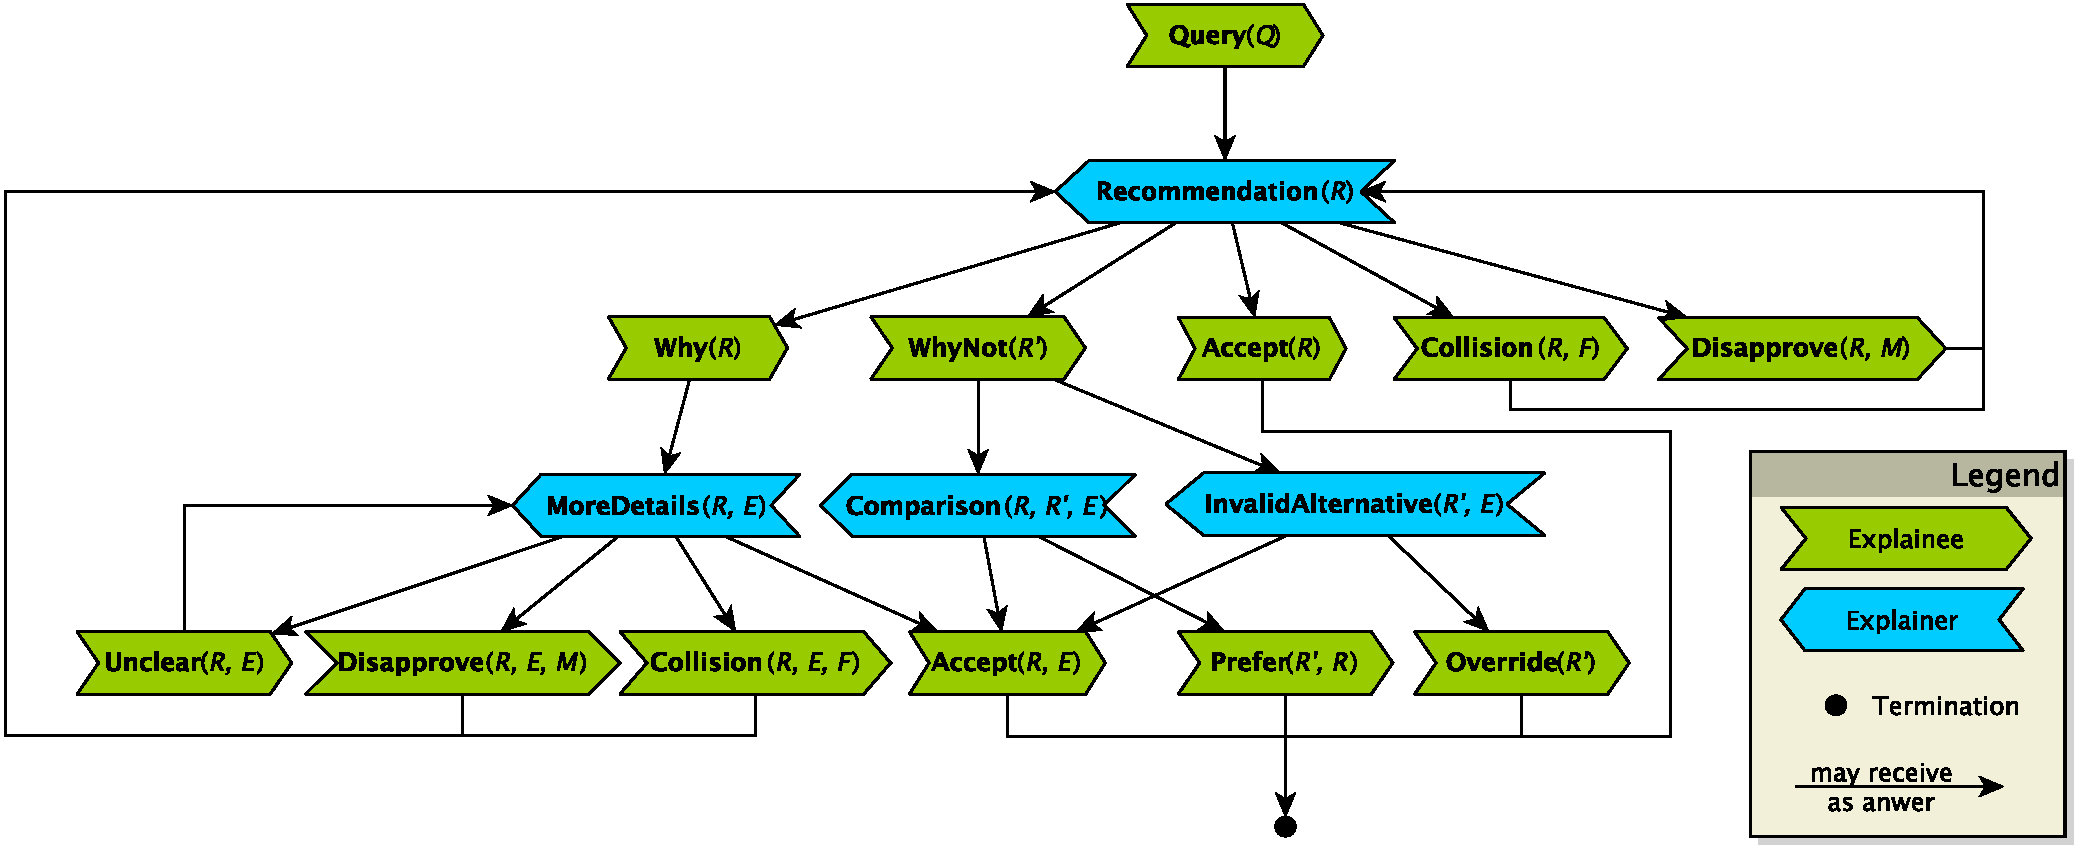
\includegraphics[width=\linewidth]{figures/pyxmas/user-agent-protocol}
    \caption[Message communication diagram between an explainer agent and an explainee]{%
      Message communication diagram between an explainer agent (blue boxes) and an explainee (green boxes).
      %
      Each box represents a message.
      %
      Arrows indicate the possible replies to each message.
    }
    \label{fig:protocol-messages}
\end{figure}
%
\Cref{fig:protocol-messages} presents an abstract formulation of the proposed protocol, which is independent of the specific representation or computation of recommendations and explanations.
%
The focus is on the exchange of messages between the explainer and the explainee, the information these messages carry, and the sequence in which they are exchanged.
%
The protocol defines two roles:
%
\begin{itemize}
    \item The explainee, who initiates the interaction.
    %
    \item The explainer, who responds to the explainee's queries.
\end{itemize}
%
Five data types are identified as the potential payloads exchanged during the protocol:
%
\begin{itemize}
    \item \textbf{Queries} (\(Q\)): Requests for recommendations submitted by the explainee.
    %
    \item \textbf{Recommendations} (\(R, R'\)): Responses to queries, provided by the explainer.
    %
    \item \textbf{Explanations} (\(E, E'\)): Information provided by the explainer to clarify recommendations.
    %
    \item \textbf{Features} (\(F\)): User-specific aspects that justify the rejection of a recommendation, which the explainer should consider in future interactions.
    %
    \item \textbf{Motivations} (\(M\)): Reasons for rejecting a recommendation, which may influence the explainer's behavior.
\end{itemize}
%
Thirteen message types are defined, each represented as a named record of the form \texttt{Name(Payload)}, where \texttt{Payload} consists of instances of the aforementioned data types.
%
Optional fields in the payload are denoted with a question mark.
%
The message types are summarized as follows:
%
\begin{enumerate}
    \item \texttt{Query(\(Q\))}: Sent by the explainee to initiate the protocol, carrying a recommendation request.
    %
    \item \texttt{Recommendation(\(Q, R\))}: Sent by the explainer in response to a query, carrying the query and the computed recommendation.
    %
    \item \texttt{Why(\(Q, R\))}: Sent by the explainee to request an explanation for a recommendation.
    %
    \item \texttt{WhyNot(\(Q, R, R'\))}: Sent by the explainee to request a contrastive explanation, comparing the recommendation with an alternative.
    %
    \item \texttt{Accept(\(Q, R, E?\))}: Sent by the explainee to accept a recommendation, optionally including the explanation.
    %
    \item \texttt{Collision(\(Q, R, F, E?\))}: Sent by the explainee to notify the explainer of a conflict between the recommendation and a personal feature.
    %
    \item \texttt{Disapprove(\(Q, R, M, E?\))}: Sent by the explainee to reject a recommendation, providing a reason and optionally the explanation.
    %
    \item \texttt{Details(\(Q, R, E\))}: Sent by the explainer to provide additional details about a recommendation.
    %
    \item \texttt{Comparison(\(Q, R, R', E\))}: Sent by the explainer to provide a contrastive explanation when the alternative recommendation is also valid.
    %
    \item \texttt{Invalid(\(Q, R', E\))}: Sent by the explainer to indicate that the alternative recommendation is invalid, with an explanation.
    %
    \item \texttt{Unclear(\(Q, R, E\))}: Sent by the explainee to indicate that the provided explanation is unclear.
    %
    \item \texttt{Prefer(\(Q, R, R'\))}: Sent by the explainee to express a preference for an alternative recommendation.
    %
    \item \texttt{Override(\(Q, R, R'\))}: Sent by the explainee to enforce an alternative recommendation, even if deemed invalid by the explainer.
\end{enumerate}
%
This abstract formulation ensures flexibility, allowing implementers to tailor the protocol to specific application domains.

Notably, messages are designed by keeping the \gls{ReST} [9] architectural style into account.
%
Hence, each message type is designed to carry all the information necessary for any involved party to decide which action to take next.
%
This is the reason why all/most messages carry the original query $Q$ and the recommendation $R$ (or $R'$) which they are referring to.
%
The message communication diagram from \Cref{fig:protocol-messages} depicts not only the messages exchanged by the explainee and explainer, but also the admissbile request-response patterns which the protocol allows.
%
There, a more detailed view of the message flow is provided, which we briefly summarise in the following.


\subsubsection{Relevant scenarios and protocol analysis}\label{subsubsec:relevant-scenarios}
%
% !TeX spellcheck = en_GB
% !TeX root = ../phd-thesis.tex

\begin{figure}
    \centering{
        \begin{subfigure}[t]{0.4\linewidth}
            \centering
            \includegraphics[width=\linewidth]{figures/quick-accept}
            \caption{Quick accept: the user accepts the recommendation without asking for explanations.}
            \label{fig:quick-accept}
        \end{subfigure}
        \hfill%\vline\hfill
        \begin{subfigure}[t]{0.4\linewidth}
            \centering
            \includegraphics[width=\linewidth]{figures/quick-retry}
            \caption{Quick retry: the user rejects the recommendation without asking for explanations. Another recommendation is proposed, accordingly.}
            \label{fig:quick-retry}
        \end{subfigure}
    }

    \medskip

    \centering{
        \begin{subfigure}[t]{0.4\linewidth}
            \centering
            \includegraphics[width=\linewidth]{figures/explanation-loop}
            \caption{Ordinary explanation loop: the user asks `why' after a recommendation, and then agent answers with further details. The request for details may be repeated several times.}
            \label{fig:explanation-loop}
        \end{subfigure}
        \hfill%\vline\hfill
        \begin{subfigure}[t]{0.4\linewidth}
            \centering
            \includegraphics[width=\linewidth]{figures/contrastive-explanation-loop}
            \caption{Contrastive explanation loop: the user asks `why not' another recommendation. The agent may then explain why the other recommendation is acceptable or invalid. The user may either accept the original recommendation or prefer their own.}
            \label{fig:contrastive-explanation-loop}
        \end{subfigure}
    }
    \caption{Sequence diagrams describing most common scenarios of the protocol.}
    \label{fig:protocol-sequence-diagrams}
\end{figure}

%
The proposed protocol is versatile and accommodates various user needs and desires.
%
These include:
%
\begin{inlinelist}
    \item requesting a recommendation,
    \item seeking an explanation for the recommendation,
    \item asking for additional details about the explanation,
    \item simulating alternative recommendations, and
    \item providing feedback on recommendations or explanations.
\end{inlinelist}
%
\Cref{fig:protocol-sequence-diagrams} illustrates these scenarios, which are detailed below.

%
\paragraph{Quick Accept}
%
In this scenario, depicted in \Cref{fig:quick-accept}, the user accepts the recommendation without requiring an explanation.
%
For example, a user requests a restaurant recommendation, and the agent suggests a restaurant that the user finds satisfactory.

%
\paragraph{Quick Retry}
%
In \Cref{fig:quick-retry} the user rejects the recommendation without asking for an explanation.
%
The rejection may occur because the recommendation conflicts with the user's preferences or is unsuitable for the current context.
%
For instance, if the agent recommends a steakhouse to a vegetarian user, the user may signal a conflict with their preferences.
%
Alternatively, the user may simply disapprove of the recommendation without providing specific feedback.
%
In both cases, the agent generates a new recommendation.
%
The agent is expected to learn from conflicts but not from generic disapprovals.

%
\paragraph{Ordinary Explanation Loop}
%
In the case shown in \Cref{fig:explanation-loop}, the user requests an explanation for the recommendation.
%
If the explanation is unsatisfactory, the user may ask for further details, initiating an iterative process.
%
This loop continues until the user either accepts the recommendation or requests a new one.
%
The protocol supports ``zooming'' explanations, where the agent adjusts the granularity of the explanation.
%
For example, the agent may first provide local explanations, describing how the specific recommendation was generated.
%
Subsequently, it may offer global explanations, detailing the general logic behind its recommendations.
%
The agent can also switch between textual and visual explanations to enhance clarity.
%
Consider a user who requests a restaurant recommendation.
%
The agent suggests an Asian restaurant with a high rating and proximity to the user.
%
If the user asks for an explanation, the agent may state that the restaurant matches the user's taste for sushi and is within 1 km.
%
If further details are requested, the agent may explain its general recommendation strategy, such as prioritizing highly rated restaurants within a certain distance.

%
\paragraph{Contrastive Explanation Loop}
%
Lastly, in \Cref{fig:contrastive-explanation-loop}, the user requests a contrastive explanation, comparing the given recommendation \(R\) with an alternative \(R'\).
%
If \(R'\) is valid, the agent provides a comparison, highlighting why one recommendation is preferable.
%
If \(R'\) is invalid, the agent explains why it cannot be recommended.
%
The user may then accept the original recommendation, prefer the alternative, or override the agent's decision.
%
For example, if the agent recommends an Asian restaurant, but the user prefers a steakhouse, the agent may compare the two options.
%
If the steakhouse aligns with the user's dietary goals, the agent may note that the Asian restaurant is closer.
%
If the steakhouse violates dietary goals, the agent explains this conflict.
%
In either case, the user decides whether to accept the original recommendation or override it.
%
The agent learns from overrides to refine future recommendations.


\subsubsection{Which Sorts of Explanations and Recommendations?}
\label{subsubsec:which-sorts-of-explanations-and-recommendations}

The proposed explanation protocol is agnostic regarding the specific representation of explanations and recommendations.
%
It is the responsibility of the implementer to define how explanations and recommendations are represented and computed.
%
The protocol only specifies \emph{when} these elements should be computed.

\Glspl{RS} typically rely on one or more \gls{ML} predictors trained on user data.
%
Whether the training of these predictors is performed by the recommender agent or if the agent is equipped with pre-trained predictors at deployment is an implementation detail.
%
In either case, the recommender agent must have access to user profile information.
%
This information can be obtained during an initial configuration phase or inferred from user interactions, such as accepted or rejected recommendations.
%
To support dynamic learning, the agent should include a learning algorithm capable of updating the predictors when new user data becomes available.
%
From this perspective, the explainer agent acts as a proxy for the \gls{ML} predictor(s).

Explanations, however, are not necessarily derived from \gls{ML} predictors.
%
The \gls{XAI} literature offers a wide range of approaches for generating explanations, including visual, textual, and numerical methods~\cite{DBLP:journals/inffus/ArrietaRSBTBGGM20,DBLP:journals/csur/GuidottiMRTGP19,DBLP:journals/csur/CiattoSAMO24}.
%
The explainer agent must not only wrap the \gls{ML} predictor(s) but also encapsulate the logic for computing and representing explanations.

A critical challenge arises when recommendations and explanations use different representation formats, such as textual and visual.
%
In such cases, the explainer agent must bridge the gap by providing a unified representation of both the recommendation and its explanation.
%
To address this, designers may consider adopting computational logic as a unifying framework for recommendations and explanations.
%
In computational logic, both knowledge bases and queries are represented as logic formulas.
%
These formulas can be used to represent recommendation requests, solutions, and explanations.

For example, a recommendation query can be expressed as the logic goal:
%
\[
\texttt{should\_eat(Food, lunch)},
\]
%
where \texttt{Food} is a logic variable representing an unknown value.
%
Recommendations, such as \( R, R', R'' \), correspond to logic solutions, e.g., \(\texttt{Food} = \texttt{paella}\).
%
Explanations \( E, E', E'' \) can take various forms:
%
\begin{itemize}
    \item \textbf{Local explanations:} The path in the proof tree computed by the explainer agent to derive the recommendation.
    %
    \item \textbf{Global explanations:} The logic program used by the explainer agent to generate the recommendation.
    %
    \item \textbf{Contrastive explanations:} Metrics comparing multiple recommendations or identifying constraints that make certain recommendations invalid.
    %
    \item \textbf{Combinations:} Any combination of the above types.
\end{itemize}

User features, such as \( F, F', F'' \), may include raw facts describing the user, e.g., \texttt{age(31)}, \texttt{goal(lose\_weight)}, or \texttt{category(vegetarian)}.
%
Motivations for disapproval can include predefined facts, such as:
%
\begin{itemize}
    \item \texttt{dislike:} The user dislikes the recommendation, prompting the agent to learn from this feedback.
    %
    \item \texttt{not\_now:} The user does not want the recommendation at the moment, but may accept it in the future.
    %
    In this case, the agent should not memorize the rejection.
    %
\end{itemize}


\subsection{From Theory to Practice with \textsc{PyXMas}}
\label{subsec:from-theory-to-practice-with-pyxmas}
%
\begin{figure}
    \centering
    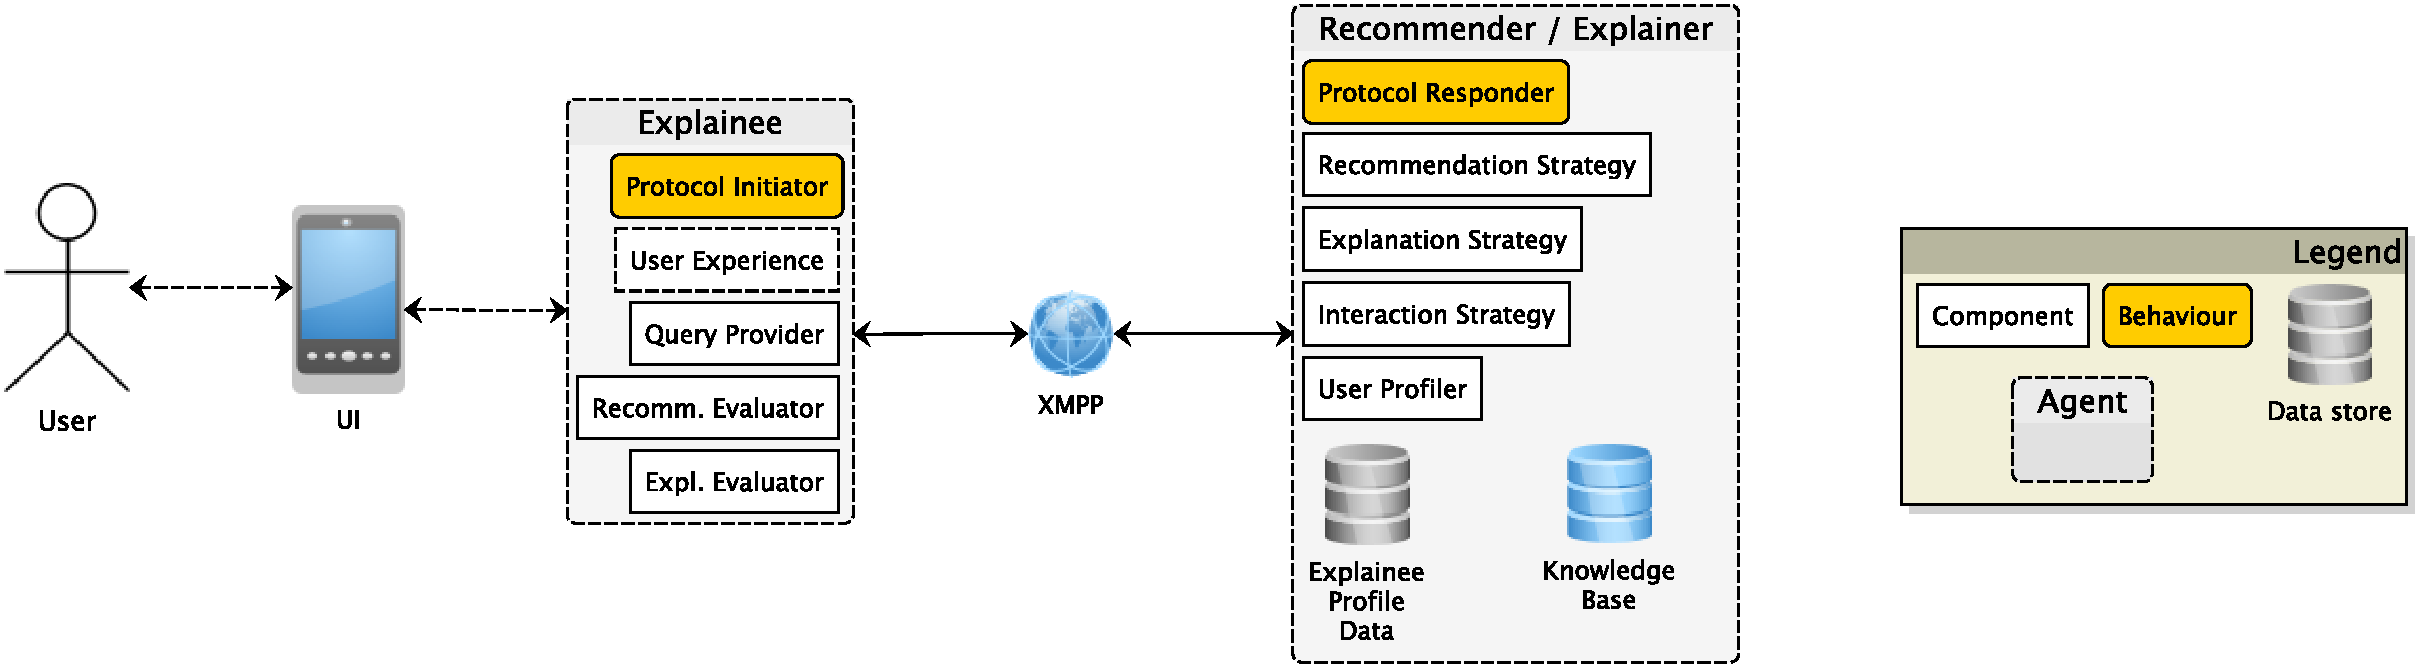
\includegraphics[width=\linewidth]{figures/pyxmas/architecture}
    \caption[Modular architecture of \textsc{PyXMas}]{%
        Modular architecture of \textsc{PyXMas}.
        %
        The library provides parametric behaviours that can be customized by implementing specific components.
        %
        If the explainee agent is human, a UX component may be required to facilitate interaction via a device.
    }
    \label{fig:architecture}
\end{figure}
%
This section describes how the proposed protocol can be implemented as agent-oriented software.
%
We introduce \textsc{PyXMas}\footnote{\url{https://github.com/pikalab-unibo/pyxmas}}, a Python library for explainable multi-agent systems (\glspl{MAS}).
%
The library is built on \textsc{Spade} and provides reusable implementations of the protocol described in \Cref{subsec:abstract-formulation-of-the-protocol}.
%
This allows researchers and developers to focus on designing recommender and explainer agents, as well as defining the representation of recommendations and explanations, without re-implementing the protocol.


\subsubsection{\textsc{PyXMas} Architecture}
\label{subsubsec:pyxmas-architecture}
%
\Cref{fig:architecture} illustrates the modular architecture of \textsc{PyXMas}.
%
The library defines two main behaviours:
%
\begin{inlinelist}
    \item the \emph{initiator}, responsible for sending recommendation queries and processing responses, and
    %
    \item the \emph{responder}, responsible for computing and returning recommendations and explanations.
\end{inlinelist}
%
The initiator behaviour is designed for the explainee agent, while the responder behaviour is intended for the explainer agent.
%
Both behaviours are parametric, allowing users to customize their functionality by implementing specific components.

\paragraph{Explainer Agent}
%
The explainer agent requires the following components:
%
\begin{itemize}
    \item \textbf{Recommendation Strategy:} Computes recommendations based on user queries, preferences, and goals (e.g., ``vegetarian'' or ``weight loss'').
    %
    The strategy can adapt over time by learning from user feedback.
    %
    \item \textbf{Explanation Strategy:} Generates explanations for recommendations, leveraging user profiles and domain knowledge (e.g., ``ingredient X is plant-based'').
    %
    \item \textbf{User Profiler:} Learns user preferences from feedback using heuristic or \gls{ML}-based methods.
    %
    This enables the agent to refine recommendations and explanations dynamically.
    %
    \item \textbf{Interaction Strategy:} Manages how recommendations and explanations are presented to the explainee.
    %
    For example, a humanoid robot may use gestures or facial expressions to enhance interaction.
\end{itemize}
%
The explainer agent stores two types of data:
%
\begin{inlinelist}
    \item user profile data, and
    %
    \item domain knowledge.
\end{inlinelist}
%
These are maintained in dedicated data stores and updated as needed.

\paragraph{Explainee Agent}
%
The explainee agent requires the following components:
%
\begin{itemize}
    \item \textbf{Query Provider:} Generates queries based on the explainee's goals.
    %
    \item \textbf{Recommendation Evaluator:} Assesses recommendations and decides whether to accept or reject them.
    %
    \item \textbf{Explanation Evaluator:} Evaluates explanations and influences the recommendation evaluator accordingly.
\end{itemize}
%
If the explainee is a human user, the agent acts as a proxy, mediating interactions via a \gls{UI} on a device (e.g., a smartphone).
%
In this case, a \textbf{\gls{UX}} component is required to manage the \gls{UI}, process user inputs, and present recommendations and explanations.


\subsubsection{PyXMas Design}\label{subsubsec:pyxmas-design}
%
\begin{figure}
    \centering
    \includegraphics[width=0.7\linewidth]{figures/pyxmas/types}
    \caption{
        Abstract classes for message payloads in \textsc{PyXMas}.
    }
    \label{fig:types}
\end{figure}
%
\textsc{PyXMas} is a Python library designed for developing explainable \glspl{MAS}.
%
It provides:
%
\begin{itemize}
    \item Abstract classes for the (de)serialization of message payloads exchanged between the explainer and explainee agents (see \Cref{fig:types}).
    %
    \item Abstract classes defining the initiator and responder behaviors.
\end{itemize}
%
These abstract classes allow developers to extend and customize their functionality by overriding specific methods.
%
This flexibility enables the creation of tailored explainable \glspl{MAS}.
%
\paragraph{Data Types for Message Payloads}
%
As illustrated in \Cref{fig:types}, \textsc{PyXMas} provides five abstract classes corresponding to the data types defined in \Cref{subsec:abstract-formulation-of-the-protocol}.
%
These classes enforce serialization, ensuring that data can be converted to and from strings.
%
This is essential for enabling communication between the explainer and explainee agents over the network.
%
Developers can define custom representations for queries, recommendations, explanations, and other data types by extending these abstract classes.
%
The only requirement is that the serialized data must be both machine- and human-readable.
%
\paragraph{Predefined Behaviors}
%
\begin{figure}
    \centering
    \begin{subfigure}[t]{\linewidth}
        \centering
        \includegraphics[width=\linewidth]{figures/pyxmas/user-state-diagram}
        \caption{
            Initiator-side state diagram.
        }
        \label{fig:user-state-diagram}
    \end{subfigure}
    %
    \begin{subfigure}[t]{\linewidth}
        \centering
        \includegraphics[width=\linewidth]{figures/pyxmas/agent-state-diagram}
        \caption{
            Responder-side state diagram.
        }
        \label{fig:agent-state-diagram}
    \end{subfigure}
    \caption{
        State diagrams describing the initiator and responder behaviors in \textsc{PyXMas}.
    }
    \label{fig:state-diagrams}
\end{figure}
%
\textsc{PyXMas} provides two abstract classes for the protocol roles:
%
\begin{itemize}
    \item The \emph{initiator}, which represents the explainee agent.
    %
    \item The \emph{responder}, which represents the explainer agent.
\end{itemize}
%
These behaviors are implemented as finite-state machines (FSMs) using \textsc{Spade}.
%
Each state corresponds to a specific action, such as waiting for a message or processing a response.
%
\Cref{fig:state-diagrams} illustrates the state diagrams for the initiator and responder behaviors.
%
On the initiator side, developers can override callbacks to control:
%
\begin{itemize}
    \item Query generation.
    %
    \item Evaluation of recommendations and decisions to accept or reject them.
    %
    \item Evaluation of explanations and their influence on recommendation acceptance.
\end{itemize}
%
On the responder side, developers can override callbacks to control:
%
\begin{itemize}
    \item Recommendation generation.
    %
    \item Explanation generation.
    %
    \item Handling of accepted or rejected recommendations.
\end{itemize}
%
This design ensures that \textsc{PyXMas} can be adapted to various application domains while maintaining a clear and modular structure.


\section[\Gls{NeSy} \Gls{AI} for disease diagnosis and monitoring]{\Gls{NeSy} \gls{AI} for supporting Chronic disease diagnosis and monitoring}
\label{sec:nesy-ai-for-supporting-chronic-disease-diagnosis-and-monitoring}
%
\subsection{Motivations and background}
\label{subsec:motivations-and-background}
%
Telemedicine platforms are increasingly used for personal assistance, enabling patients to share their symptoms, medical history, and diagnostic data, such as medical images, lab results, or vital signs.
%
These platforms often leverage \gls{AI} data-driven models~\cite{HunterNEJMra2212850,topol2022}.
%
While promising, accurate disease monitoring and diagnosis require more than identifying patterns in data.
%
The integration of \gls{AI} into clinical practice remains limited due to several challenges.
%
First, the performance of \gls{AI} models is often suboptimal, primarily due to insufficient dataset sizes for effectively training \gls{ML} algorithms~\cite{benjamens2020state}.
%
Second, even high-performing \gls{AI} models frequently operate as black boxes, making their outputs difficult to interpret.
%
This lack of transparency hinders adoption in clinical settings, where healthcare professionals require interpretable outputs to make informed decisions~\cite{ALI2023107555}.
%
Traditional clinical protocols, while validated and robust, also exhibit limitations.
%
They often fail to classify all clinical cases, leaving certain scenarios unresolved.
%
Additionally, these protocols do not leverage data analytics, which could uncover hidden patterns and provide valuable insights for decision-making.

Combining data-driven and knowledge-based models has been identified as a promising solution to enhance \gls{ML} performance and improve explainability~\cite{von2021informed}.
%
This work focuses on \gls{NeSy} \gls{AI}, specifically \gls{SKI}~\cite{DBLP:journals/csur/CiattoSAMO24}.
%
Among the various \gls{SKI} methods, we evaluate the \gls{LTN} approach~\cite{BadreddineGSS22}.
%
The potential of this approach is demonstrated using the \gls{PID} dataset for diabetes prediction~\cite{smith1988using}.
%
We compare its performance against classical \gls{ML} models, including \gls{KNN}, \gls{LR}, \gls{DT}, \gls{RF}, and an uneducated \gls{MLP}.
%
Performance is evaluated based on criteria such as classification accuracy and robustness.

Results indicate that classical \gls{ML} models struggle to achieve consistent performance.
%
In contrast, injecting domain knowledge into neural networks via the \gls{LTN} method significantly improves clinically relevant metrics, such as recall, balanced accuracy, F1 score, and Matthews Correlation Coefficient~\cite{MATTHEWS1975442}.
%
Moreover, \gls{LTN} enhances adherence to clinical knowledge, a critical requirement in the medical domain.
%
It also demonstrates high robustness against data manipulation, including noise injection, data dropping, and label flipping.

\subsection{Knowledge integration in medicine}
\label{subsec:knowledge-integration-in-medicine}

The integration of medical knowledge into \gls{ML} pipelines can occur at various stages~\cite{von2021informed,kierner2023taxonomy}.
%
\begin{itemize}
    \item \textbf{Data pre-processing:} Errors in datasets can be mitigated by removing anomalous samples based on clinical norms.
    %
    Virtual samples adhering to medical knowledge can be generated to address insufficient or missing data.
    %
    \item \textbf{Feature engineering:} Novel features can be derived using mathematical or logical models informed by medical knowledge.
    %
    Feature selection can also be guided by prior knowledge.
    %
    \item \textbf{Model learning:} Rules can be incorporated into the model's loss function or architecture.
    %
    \item \textbf{Output evaluation:} \gls{ML} outputs can be integrated with clinical guidelines to filter predictions or verify consistency with domain knowledge.
\end{itemize}
%
While these strategies are promising, they often do not reference the \gls{SKI} framework or its complementary \gls{SKE} paradigm~\cite{DBLP:journals/csur/CiattoSAMO24}.
%
These paradigms have proven effective in other domains and hold potential for healthcare applications.
%
Preliminary experiments~\cite{sirocchiRuleML2024} suggest that further evaluation of \gls{SKI} methods, such as \gls{LTN}, is warranted.


\subsection{Materials and methods}
\label{subsec:materials-and-methods}
%
In this study, we utilize the \gls{PID} dataset~\footnote{\url{https://www.kaggle.com/datasets/uciml/pima-indians-diabetes-database}}, a widely recognized benchmark in medical-related \gls{ML} research~\cite{karegowda2011application,DBLP:journals/nca/ChangBXS23}.
%
We focus on the \gls{LTN} approach~\cite{BadreddineGSS22}, a \gls{SKI} method that combines structuring and constraining injection strategies.
%
This section details the dataset, the \gls{LTN} methodology, and the metrics used to evaluate the impact of \gls{SKI} on predictive performance and \gls{QoS} aspects.

%
\subsubsection{Dataset and knowledge}
\label{subsubsec:dataset-and-knowledge}
%
The \gls{PID} dataset consists of 768 medical profiles of women aged 21 and above who underwent an oral glucose tolerance test.
%
The dataset includes features such as glucose and insulin concentrations, blood pressure (BP), skin thickness (ST), body mass index (BMI), diabetes pedigree function, number of pregnancies, and age.
%
The target variable is binary, indicating whether diabetes was diagnosed within five years.

%
Missing values are present in several attributes, including insulin (48.70\%), ST (29.56\%), BP (4.55\%), BMI (1.43\%), and glucose (0.65\%).
%
These missing values were imputed using the median value of the respective attribute.
%
The dataset is imbalanced, with 65.1\% of instances labeled as negative and 34.9\% as positive.

%
Public health guidelines on type-2 diabetes risks indicate that individuals with a high BMI (\(\geq 30\)) and high blood glucose levels (\(\geq 126\)) are at severe risk for diabetes.
%
Conversely, individuals with a normal BMI (\(\leq 25\)) and low blood glucose levels (\(\leq 100\)) are less likely to develop diabetes.
%
These guidelines are encoded into logic formulas as follows:
%
\begin{align}
    \forall x.\, (\text{glucose}(x) \geq 125 \land \text{bmi}(x) \geq 30 \rightarrow \text{Diabetic}(x)), \label{eq:diabetes_rule1} \\
    \forall x.\, (\text{glucose}(x) \leq 100 \land \text{bmi}(x) \leq 25 \rightarrow \neg \text{Diabetic}(x)). \label{eq:diabetes_rule2}
\end{align}

%
\subsubsection{Logic Tensor Network for \gls{SKI}}
\label{subsubsec:ltn-for-ski}
%
The \gls{LTN} framework~\cite{BadreddineGSS22} extends \gls{FOL} with fuzzy semantics, where formulas are interpreted as continuous truth values in the interval \([0, 1]\).
%
This allows the definition of logic rules that are not strictly true or false but partially true, with predicates computed by neural networks.

%
In this study, we use \gls{LTN} to inject the knowledge encoded in Equations~\eqref{eq:diabetes_rule1} and~\eqref{eq:diabetes_rule2}.
%
The predicate \(\text{Diabetic}(x)\) is modeled as a neural predicate backed by a feed-forward \gls{NN} with three hidden layers.
%
The NN outputs a real number in \([0, 1]\), representing the truth value of \(\text{Diabetic}(x)\) for an input \(x \in \mathbb{R}^8\).

%
The training process maximizes the truth value of the logic formulas while considering the available data.
%
This is achieved by minimizing a loss function that penalizes violations of the injected knowledge.
%
The predicates \(\text{glucose}(x)\) and \(\text{bmi}(x)\) are grounded to the actual values in the dataset, while the following dummy formulas are added to supervise the training:
%
\begin{align}
    \forall x.\, (\text{outcome}(x) = \text{diabetes} \rightarrow \text{Diabetic}(x)), \\
    \forall x.\, (\text{outcome}(x) = \text{healthy} \rightarrow \neg \text{Diabetic}(x)).
\end{align}

%
\subsubsection{Evaluation Metrics}
\label{subsubsec:evaluation-metrics}
%
To assess the impact of \gls{SKI}, we evaluate both predictive performance and \gls{QoS} metrics.

%
\paragraph{Performance Metrics}
%
Predictive performance is evaluated using standard metrics for binary classification, including accuracy, precision, recall, F1-score, balanced accuracy (BA), and the \gls{MCC}.

%
\paragraph{Logic Adherence}
%
Inspired by fidelity metrics in the \gls{SKE} framework~\cite{DBLP:journals/csur/CiattoSAMO24}, we propose a metric to assess adherence to clinical rules.
%
For each rule, we create a test set of instances satisfying the rule, assign labels based on the rule, and compute the model's accuracy on this subset.

%
\paragraph{Quality of Service}
%
\gls{QoS} metrics evaluate non-functional aspects such as robustness and complexity.
%
This study focuses on robustness to data degradation, which occurs when input data is noisy, incomplete, or biased.
%
Robustness is quantified using a reproducible procedure where training data is perturbed, and the model's performance is evaluated on the perturbed data~\cite{DBLP:journals/aamas/AgiolloRMCO23}.
%
The robustness score \(\rho_{N, D}(D)\) of a predictor \(N\) trained on \(D\) is defined in \Cref{eq:robustness-score}.
%
The robustness gain \(R_{N, D}(I)\) of an injection mechanism \(I\) is computed as shown in \Cref{eq:robustness-gain}.
%
A value \(R_{N, D}(I) > 1\) indicates improved robustness, while \(R_{N, D}(I) < 1\) indicates reduced robustness.


\subsubsection{Experimental Design}
\label{subsubsec:experimental-design}
%
The experiments are designed to evaluate the impact of the \gls{LTN} approach on the performance of \gls{ML} models in a clinical context.
%
The implementation of \gls{LTN} used in this study is publicly available\footnote{\url{https://github.com/pikalab-unibo/experiments-ltn-2024}}, along with the code for replicating the experiments.
%
The evaluation focuses on three main aspects:
%
\begin{enumerate}
    \item The predictive performance of \gls{ML} models, with particular attention to recall and F1-score, given the medical domain's sensitivity to false negatives.
    %
    \item The adherence of \gls{ML} models to established medical protocols, assessing whether the educated model aligns more closely with the injected knowledge compared to the uneducated one.
    %
    \item The robustness of \gls{ML} models to data degradation, analyzing whether the performance of the educated model degrades less than that of the uneducated model under perturbed data.
\end{enumerate}
%
To ensure a fair comparison, a grid search is performed to optimize the hyperparameters of all models.
%
The best hyperparameters for the baseline models are as follows:
%
\begin{itemize}
    \item \gls{KNN}: \(k = 7\), L1 distance.
    %
    \item \gls{DT}: Entropy as the split criterion, maximum depth of 10.
    %
    \item \gls{RF}: 50 trees, maximum depth of 20, entropy as the criterion, and a minimum of 5 samples per leaf.
    %
    \item \gls{LR}: Regularization parameter of 10, maximum iterations of 1,000, and \texttt{liblinear} as the solver.
\end{itemize}
%
The uneducated \gls{MLP} and the educated \gls{LTN} models share the same feedforward \gls{NN} architecture:
%
\begin{itemize}
    \item An input layer with 8 neurons, one for each feature in the dataset, using the \gls{LeakyReLU}~\cite{maas2013rectifier} activation function and batch normalization.
    %
    \item Three hidden layers with 256, 128, and 64 neurons, respectively, each using \gls{LeakyReLU} and batch normalization.
    %
    \item An output layer with a single neuron and a sigmoid activation function.
\end{itemize}
%
The training of the \gls{LTN} model consists of two phases.
%
First, the uneducated model is trained for 50 epochs using the Adam optimizer with a learning rate of \(10^{-4}\), weight decay of \(10^{-4}\), a batch size of 32, and a binary cross-entropy loss function.
%
An early stopping criterion is applied, with a patience of 5 epochs.
%
Second, the knowledge is injected, and the model is fine-tuned for 200 epochs using the same early stopping criterion but with a reduced learning rate of \(10^{-6}\).
%
All models are evaluated using multiple runs of a 50--50 train-test split, with performance metrics averaged over 50 runs.
%
Statistical significance is assessed using the Wilcoxon signed-rank test with a significance level of 0.05.
%
To evaluate robustness, the experiments include multiple runs with different types and magnitudes of data perturbations.
%
The perturbations include noise addition, sample drop, and label flipping, following the methodology in~\cite{DBLP:journals/aamas/AgiolloRMCO23}.
%
The noise magnitude \(\mu\) ranges from 0.1 to 1.0 in steps of 0.1, while the percentages of sample drop and label flipping vary from 0 to 0.9 in steps of 0.1.


\subsection{Results and Discussion}
\label{subsec:results-discussion}
%
We now present and discuss the results obtained for predictive performance metrics, logical adherence, and robustness.

%
\subsubsection{Performance Metrics}
\label{subsubsec:performance-metrics}
%
\begin{table*}[]
    \centering
    \begin{adjustbox}{max width=\textwidth}
        \begin{tabular}{|l|c|c|c|c|c|c|}
            \hline
            \textbf{Model} & \textbf{Accuracy} & \textbf{Precision} & \textbf{Recall} & \textbf{F1 Score} & \textbf{Balanced Accuracy} & \textbf{MCC} \\
            \hline
            \gls{KNN}  & 0.738 $\pm$  0.02 & 0.636 $\pm$  0.03 & 0.583 $\pm$  0.05 & 0.607 $\pm$  0.03 & 0.702 $\pm$  0.02 & 0.413 $\pm$  0.05 \\
            \hline
            \gls{DT}   & 0.697 $\pm$  0.02 & 0.565 $\pm$  0.03 & 0.580 $\pm$  0.05 & 0.571 $\pm$  0.03 & 0.670 $\pm$  0.02 & 0.339 $\pm$  0.05 \\
            \hline
            \gls{RF}   & 0.758 $\pm$  0.02 & 0.677 $\pm$  0.03 & 0.592 $\pm$  0.05 & 0.630 $\pm$  0.03 & 0.720 $\pm$  0.02 & 0.456 $\pm$  0.04 \\
            \hline
            \gls{LR}   & \textbf{0.763 $\pm$  0.02 }& \textbf{0.702 $\pm$  0.04} & 0.560 $\pm$  0.04 & 0.622 $\pm$  0.03 & 0.716 $\pm$  0.02 & 0.460 $\pm$  0.04 \\
            \hline
            \gls{MLP}  & 0.754 $\pm$  0.02 & 0.644 $\pm$  0.03 & 0.665 $\pm$  0.05 & 0.653 $\pm$  0.03 & 0.733 $\pm$  0.02 & 0.464 $\pm$  0.04 \\
            \hline
            \gls{LTN}  & 0.747 $\pm$  0.02 & 0.620 $\pm$  0.03 & \textbf{0.725 $\pm$  0.05} & \textbf{0.666 $\pm$  0.02} & \textbf{0.742 $\pm$  0.02} & \textbf{0.471 $\pm$  0.03} \\
            \hline
        \end{tabular}
    \end{adjustbox}
%    \vspace{0.5em}
    \caption[Performance metrics for \glsentryshort{ML} models on the \glsentryshort{PID} Dataset]{
      Performance metrics (mean $\pm$ std) for \glsentryshort{ML} models.
      %
      The best scores are highlighted in bold.
      %
      According to the Wilcoxon signed-rank test with p-value=0.05, the \gls{LTN} model outperforms all other models in terms of Recall, F1 Score, and Balanced Accuracy.
    }
    \label{tab:ski-diabetes-performance-metrics}
%    \vspace{-3em}
\end{table*}
%
The performance metrics are summarized in \Cref{tab:ski-diabetes-performance-metrics}.
%
While \gls{LR} achieves the highest accuracy, this metric is less reliable for imbalanced datasets.
%
In this study, the minority class, representing diabetic instances, is the primary focus.
%
The \gls{LTN} model achieves the highest scores in balanced accuracy, F1-score, and \gls{MCC}.
%
These metrics are more suitable for evaluating clinical models as they account for class imbalance.
%
The \gls{LTN} also achieves the highest recall value of \(0.725\), which is critical in clinical settings.
%
Recall measures the proportion of diabetic patients correctly identified, minimizing false negatives.
%
False negatives can lead to missed diagnoses and untreated conditions, which are particularly problematic in healthcare.
%
In contrast, \gls{KNN} and \gls{DT} achieve recall values of \(0.583\) and \(0.580\), respectively, indicating their limited ability to detect positive cases.
%
\gls{LR} achieves a recall of \(0.560\), while \gls{RF} slightly improves with a recall of \(0.592\).
%
Although the \gls{MLP} shows some improvement with a recall of \(0.66\), the injection of domain knowledge via the \gls{LTN} yields a significant performance boost.
%
Precision, while highest for \gls{LR}, is less emphasized in clinical contexts, as false positives typically lead to follow-up testing with minimal consequences.
%
These results highlight the limitations of classical \gls{ML} models in achieving sufficient recall for clinical deployment.
%
The superior recall of the \gls{LTN} can be attributed to its incorporation of logic formulas, which effectively utilize background knowledge.
%
By grounding predictions in logical structures, the \gls{LTN} identifies patterns that simpler models may overlook.

%
\subsubsection{Logical Adherence}
\label{subsubsec:logical-adherence}
%
\begin{table}
  \centering
  \begin{adjustbox}{max width=0.8\textwidth}
    \begin{tabular}{|l|c|c|}
      \hline
      \textbf{Model} & \textbf{Rule 1} & \textbf{Rule 2} \\
      \hline
      \gls{KNN}  & 70.8 $\pm$  4.8   & 100.0 $\pm$  0.0 \\
      \hline
      \gls{DT}   & 66.5 $\pm$  6.3   & 97.0 $\pm$  4.8 \\
      \hline
      \gls{RF}   & 76.6 $\pm$  5.1   & 100.0 $\pm$  0.0 \\
      \hline
      \gls{LR}   & 75.0 $\pm$  4.2   & 100.0 $\pm$  0.0 \\
      \hline
      \gls{MLP}  & 82.0 $\pm$  5.8   & 100.0 $\pm$  0.0 \\
      \hline
      \gls{LTN}  & \textbf{87.4 $\pm$  5.2 }  & 100.0 $\pm$  0.0 \\
      \hline
    \end{tabular}
  \end{adjustbox}
%  \vspace{0.5em}
  \caption[Logic adherence results for diabetes rules]{
      Logic adherence results for \Cref{eq:diabetes_rule1} and \Cref{eq:diabetes_rule2} (mean $\pm$ std) across various models.
  }
  \label{tab:logic-adherence}
%  \vspace{-2em}
\end{table}
%
In clinical applications, models must not only make accurate predictions but also align with established medical protocols.
%
Adherence to clinical guidelines enhances trust and reliability, increasing the likelihood of adoption in practice.
%
The logical adherence results are presented in \Cref{tab:logic-adherence}.
%
All models, except for \gls{DT}, fully comply with the second rule, which classifies healthy patients.
%
However, the primary focus is on adherence to the first rule, which identifies diabetic patients.
%
The \gls{MLP} achieves \(82\%\) adherence to the first rule, outperforming classical \gls{ML} models such as \gls{RF}, which achieves \(76\%\).
%
The \gls{LTN} further improves adherence, achieving \(87\%\).
%
These results confirm that injecting domain knowledge through the \gls{LTN} modifies the model's structure, aligning it more closely with medical knowledge and clinical protocols.

%
\subsubsection{Robustness Analysis}
\label{subsubsec:robustness-analysis}
%
\begin{figure}
    \centering
    \includegraphics[width=\linewidth]{figures/ski-diabetes-robustness}
    \caption[Robustness analysis under noise injection, label flipping, and data dropping]{
        %
        Robustness analysis under noise injection, label flipping, and data dropping.
        %
        The \gls{LTN} demonstrates superior robustness across all metrics compared to other models.
    }
    \label{fig:robustness-analysis}
\end{figure}
%
Robustness refers to the model's ability to maintain performance under data perturbations, such as noise, missing data, or label flipping.
%
This evaluation is critical in clinical settings, where data collection is often noisy or incomplete.
%
The robustness results are illustrated in \Cref{fig:robustness-analysis}.
\note{TODO: generate again the figure because it is not vectorial and it has an error}
%
Under noise injection, the \gls{LTN} demonstrates the most stable performance across \gls{MCC}, balanced accuracy, F1-score, and recall.
%
Performance declines significantly only at noise levels above \(0.5\), which are uncommon in clinical environments.
%
For label flipping, the \gls{LTN} shows resilience up to a flipping rate of \(0.6\), with recall remaining virtually unchanged.
%
A notable drop is observed only at a flipping rate of \(0.7\), which is rare in practice.
%
In the case of data dropping, all models maintain stable performance up to a drop rate of \(0.8\).
%
However, the \gls{LTN} uniquely preserves recall, highlighting its ability to recover positive cases even with missing data.
%
These findings underscore the advantages of knowledge injection via the \gls{LTN}, which enhances robustness in complex clinical data scenarios.


%\subsection{\Gls{LLM}-based solutions for healthcare chatbots: a comparative analysis}\label{subsec:llm-based-solutions-for-healthcare-chatbots-a-comparative-analysis}

%\subsection{Open-source small language models for personal medical assistant chatbots}\label{subsec:open-source-small-language-models-for-personal-medical-assistant-chatbots}

\section[RAG on open LLM for medical chatbot]{Applying \glsentryshort{RAG} on open \glspl{LLM} for a medical chatbot supporting hypertensive patients}\label{sec:applying-rag-on-open-llm-for-a-medical-chatbot-supporting-hypertensive-patients}

\subsection{Motivations and Background}
\label{subsec:motivations-and-background-rag}
%
Managing chronic diseases, such as hypertension, poses significant challenges for both healthcare systems and patients.
%
These conditions require continuous monitoring, lifestyle adjustments, and often lead to substantial healthcare costs.
%
Frequent interactions with healthcare professionals can result in long wait times and limited accessibility for patients.
%
To address these issues, we propose the development of a chatbot to support patients in the self-management of chronic conditions, with a specific focus on hypertension.
%
The chatbot aims to empower hypertensive patients by providing timely, accurate, and empathetic guidance, particularly for acquiring vital signs and maintaining a healthy lifestyle~\cite{telmed2024,llm-goodit2023}.
%
Two critical requirements emerge for such a system.
%
First, the interaction must be empathetic to ensure patient engagement and motivation.
%
Second, the chatbot must provide highly accurate information, as no healthcare professional mediates the conversation.
%
Additionally, the system must comply with data privacy regulations, precluding the use of third-party systems for \gls{NLP} and \gls{NLG}.

%
Given these requirements, we consider \glspl{LLM} as the core technology for the chatbot.
%
\Glspl{LLM} have demonstrated the ability to generate trustworthy, reliable, and empathetic text, making them suitable for this application.
%
For instance, studies have shown that patients often prefer responses generated by \glspl{LLM} over those from physicians in online forums, rating the chatbot's quality and empathy higher~\cite{Chatbot-JAMAIntMed2023}.
%
To avoid reliance on proprietary third-party services, we focus on open \glspl{LLM}, including both domain-specific and general-purpose models.
%
To enhance their performance, we integrate \gls{RAG} techniques~\cite{Lewis-NIPS20}.
%
\Gls{RAG} enriches the \gls{LLM} with symbolic knowledge, which aligns with the definition of \gls{SKI} provided by~\cite{DBLP:journals/csur/CiattoSAMO24}.
%
Unlike traditional \gls{SKI} methods that rely on logic rules, \gls{RAG} incorporates symbolic knowledge in the form of free text, enabling the \gls{LLM} to generate contextually relevant and precise responses.

%
The \gls{RAG} approach involves constructing a knowledge base -- usually stored in a vectorial data base -- from data provided by medical professionals and enriching it with retrieval techniques.
%
This allows for a comprehensive comparison of retrieval strategies and \glspl{LLM}, both specialized and general-purpose.
%
Our findings demonstrate that \gls{RAG} significantly improves model performance, often surpassing specialized models in most tested cases.

%
\subsubsection{Applications of \Glspl{LLM} in Healthcare}
%
The adoption of \glspl{LLM} in healthcare has grown exponentially, with applications spanning patient care, research, and education.
%
In patient care, \glspl{LLM}-based chatbots can assist healthcare professionals by abstracting key results from literature, detecting medical errors, and supporting clinical decisions.
%
For patients, these chatbots can provide trustworthy and empathetic answers, resembling a dialogue with a physician, and proactively suggest actions based on tracked activities and vital signs.
%
In research, \glspl{LLM} can automate tasks such as data analysis, summarization, and literature search.
%
In education, they can serve as interactive tutors, providing teaching material and demonstrating strong performance in medical examinations.

%
\subsubsection{Challenges and Techniques}
%
Three key requirements must be addressed for deploying \glspl{LLM} in healthcare.
%
First, ethical concerns, including privacy and security risks, must be mitigated~\cite{lancet2023}.
%
Second, the system must be reliable, avoiding hallucinations and ensuring accuracy~\cite{EthicsLLMs-NatureDigitalMedicine2024}.
%
Third, the chatbot must communicate empathetically, motivating patients and providing real-time support~\cite{Chatbot-JAMAIntMed2023}.
%
To meet these requirements, open-source \glspl{LLM} are preferred, as they allow local deployment and direct access to model weights.
%
However, open models may generate irrelevant or incomplete content, undermining trust and compliance.
%
To address these limitations, two primary techniques are recommended: \gls{RAG} and fine-tuning.
%
While fine-tuning aligns models with domain-specific datasets, \gls{RAG} dynamically updates the knowledge base, ensuring relevance to recent information.

%
\subsubsection{\Gls{RAG} in the Medical Domain}
%
\Gls{RAG} represents an innovative integration of information retrieval and generative models, enabling access to a medical knowledge base for generating precise and contextually relevant responses.
%
This approach enhances the safety and effectiveness of \glspl{LLM} in healthcare, where accuracy and specificity directly impact patient care quality.
%
For example, \gls{RAG} has been used to improve \glspl{LLM} in digestive diseases~\cite{Giuf2024} and Hepatitis C management~\cite{Kresevic2024-NPJ}, outperforming baseline models in delivering guideline-specific recommendations.
%
However, implementing \gls{RAG} in healthcare requires tailoring solutions to local needs, considering factors such as demographics, resources, and cultural practices.
%
This flexibility necessitates a modular and configurable architecture.

%
\subsubsection{Fine-Tuning in the Medical Domain}
%
Fine-tuning has demonstrated impressive results in specialized medical domains~\cite{Maharjan2024-ScientificReports}.
%
For instance, Wang et al.~\cite{Wang2023-Jamia} fine-tuned the Llama 2 model using clinical concepts from standardized vocabularies, such as the Human Phenotype Ontology (HPO), to address underdiagnosis and misdiagnosis.
%
However, due to the limited dataset size in this study, we focus on \gls{RAG}, which allows dynamic updates to the knowledge base, ensuring the model remains relevant with recent information.


\subsection{Materials and Methods}
\label{subsec:materials-and-methods-rag}

\subsubsection{Fine-Tuning}
\glspl{LLM} are initially pre-trained on large, general-purpose text corpora to predict the next token in a sequence.
%
This process equips the model with a broad understanding of language and serves as a foundation for fine-tuning.
%
Fine-tuning involves further training the model on smaller, domain-specific datasets to adapt it to specific tasks or fields.
%
This approach is computationally efficient as it leverages the model's pre-existing knowledge while refining it for specialized applications.

Full fine-tuning updates all the model's parameters to optimize its performance for a specific task.
%
While effective, this method is resource-intensive, requiring significant computational power and memory.

Parameter-efficient fine-tuning (PEFT) updates only a subset of the model's parameters, freezing the rest.
%
This reduces memory requirements while retaining the model's general linguistic knowledge.
%
Techniques such as low-rank adaptation (LoRA) and quantized LoRA (QLoRA) further minimize resource usage by refining smaller weight matrices and lowering the precision of adapter weights~\cite{DBLP:conf/iclr/HuSWALWWC22,DBLP:conf/nips/DettmersPHZ23}.
%
By selecting the appropriate fine-tuning method, models can be optimized for specific use cases while minimizing resource consumption.

\subsubsection{\gls{RAG}}
%
\begin{figure}
    \centering
    \includegraphics[width=0.8\linewidth]{figures/rag-architecture}
    \caption[\Gls{RAG} architecture]{
        \Gls{RAG} architecture.
        %
        The retriever identifies relevant information from a knowledge base, which the generator uses to produce a contextually appropriate response.
    }
    \label{fig:rag-architecture}
\end{figure}
%
Traditionally, \glspl{LLM} generate responses based solely on patterns and information learned during pre-training.
%
This limitation often results in responses lacking depth or specific knowledge.
%
\gls{RAG} addresses this by integrating external data during the response generation process.

The \gls{RAG} framework consists of two main phases:
%
\begin{enumerate}
    \item Retrieving relevant information from a large dataset or knowledge base in response to a query.
    %
    \item Using the retrieved information to guide the generation of the response.
\end{enumerate}
%
This enables software agents, such as chatbots, to provide accurate and context-specific answers by supplementing the model's internal knowledge with external information, such as private documentation or databases.

The retriever component identifies relevant information by splitting documents into smaller fragments (chunks) and converting these chunks into embedding vectors.
%
These vectors are stored in an indexed knowledge base for efficient retrieval.
%
When a query is processed, the system generates a query vector and matches it with stored document vectors using vector similarity techniques.
%
Sparse embeddings, such as those based on TF-IDF or BM25~\cite{DBLP:books/cu/LeskovecRU14,DBLP:journals/ftir/RobertsonZ09}, rely on keyword matches but may struggle with synonyms and semantic meaning.
%
Dense embeddings, generated by models like \gls{BERT}, capture deeper semantic relationships, enabling retrieval based on meaning rather than exact words~\cite{DBLP:conf/naacl/DevlinCLT19}.
%
Hybrid approaches combine both methods to balance speed and semantic depth.
%
The generator component, a \gls{LLM}, produces the final text response.
%
\Cref{fig:rag-architecture} illustrates the \gls{RAG} architecture, highlighting the interaction between the retriever and generator components.


\subsubsection{\gls{RAG} vs. Fine-Tuning}
\gls{RAG} and fine-tuning represent distinct approaches to enhancing \glspl{LLM}, each with unique advantages.
%
\begin{itemize}
    \item \textbf{Knowledge Integration vs. Task Specialization:} \gls{RAG} integrates external knowledge dynamically, enhancing versatility and ensuring up-to-date information.
    %
    Fine-tuning specializes the model for specific tasks, improving task-specific accuracy.
    %
    \item \textbf{Dynamic vs. Static Learning:} \gls{RAG} allows dynamic access to external data, while fine-tuning updates the model based on a static training cycle.
    %
    \item \textbf{Generalization vs. Customization:} \gls{RAG} preserves the model's generality, making it adaptable across tasks, whereas fine-tuning tailors the model for specific use cases.
    %
    \item \textbf{Resource Demands:} \gls{RAG} requires runtime retrieval mechanisms, while fine-tuning is resource-intensive during training but efficient during deployment.
\end{itemize}

\subsubsection{Chosen Approach}
%
\begin{table}
  \begin{tabular}{|l|p{0.7\textwidth}|}
      \hline
      \textbf{Model} & \textbf{Description} \\
      \hline
      Llama3.1 & A general-purpose \gls{LLM} based on the Llama3 architecture with 8B parameters, trained on a diverse range of text data~\cite{llama3}. \\
      \hline
      Llama3.1-Medical & A medical-domain-specific version of Llama3.1, fine-tuned on medical data to enhance its performance in healthcare applications: \url{https://ollama.com/qordmlwls/llama3.1-medical}. \\
      \hline
      Qwen2 & A general-purpose \gls{LLM} with 7B parameters, trained on 29 different languages to improve cross-lingual performance~\cite{qwen2}. \\
      \hline
      Qwen2-Medical & A medical-domain-specific version of Qwen2, fine-tuned on medical data to improve its performance in healthcare tasks: \url{https://ollama.com/echelonify/med-qwen2}. \\
      \hline
      Mistral-Nemo & A 12B parameter model with a large context window (128K tokens) developed by Nvidia: \url{https://ollama.com/library/mistral-nemo}. \\
      \hline
      Phi3 & A relatively small \gls{LLM} with 3B parameters, trained by Microsoft on filtered high-quality data~\cite{abdin2024phi3technicalreporthighly}. \\
      \hline
      Gemma2 & A 9B parameter model based on Deepmind Gemini developed by Google~\cite{gemmateam2024gemma2improvingopen}. \\
      \hline
  \end{tabular}
  \centering
  \caption{Evaluated \gls{LLM} for our study.}
  \label{tab:evaluated-llms}
\end{table}
%
This study employs \gls{RAG} techniques to enhance the performance of open \glspl{LLM} for developing a chatbot supporting hypertensive patients.
%
\gls{RAG} was chosen over fine-tuning for several reasons:
%
\begin{itemize}
    \item It dynamically integrates external data, allowing the system to adapt to diverse contexts and provide accurate information.
    %
    \item Fine-tuning requires extensive computational resources, which are currently unavailable.
    %
    \item \gls{RAG} mitigates issues such as model drift, hallucinations, and biases that can arise during fine-tuning.
\end{itemize}

\paragraph{Retrieval Strategies}
Three retrieval strategies were tested:
%
\begin{itemize}
    \item \textbf{Base Retriever:} Retrieves information based on vector similarity using maximum marginal relevance~\cite{DBLP:conf/sigir/CarbonellG98}.
    %
    \item \textbf{Multi-Query Retriever:} Enhances diversity and relevance by generating multiple queries with a \gls{LLM} and retrieving relevant chunks for each query.
    %
    \item \textbf{Ensemble Retriever:} Combines outputs from multiple retrievers, such as the base retriever and BM25, using reciprocal rank fusion~\cite{DBLP:conf/sigir/CormackCB09}.
\end{itemize}

The dataset used for \gls{RAG} consists of 1,473 question-answer pairs extracted from medical consultations.
%
The questions cover topics related to hypertension, including symptoms, causes, treatments, and lifestyle recommendations.
%
All answers, written in Italian, were reviewed by medical professionals to ensure accuracy and relevance.

The evaluated \glspl{LLM} include both general-purpose models (e.g., Llama 3.1, Qwen2, Mistral Nemo) and medical-domain-specific models (e.g., Llama 3.1-Medical, Qwen2-Medical).
%
Further details are provided in Table~\ref{tab:evaluated-llms}.


\subsection{Evaluation}
\label{subsec:evaluation-rag}

\subsubsection{Experimental Setup}
We evaluated the effectiveness of various \gls{RAG} techniques using the RAGAS framework\footnote{\url{https://docs.ragas.io/en/stable/}}.
%
This framework provides a comprehensive suite of metrics for assessing retrieval and generation aspects of \gls{LLM}-based systems.
%
Instead of partitioning the dataset into training and test sets, we leveraged an external \gls{LLM} (GPT-4o) to generate a test set of 20 question-context-answer triplets.
%
These triplets were designed to maintain statistical relevance to the original dataset.
%
We evaluated a range of state-of-the-art open-source \glspl{LLM}, both general-purpose and domain-specific, with and without \gls{RAG}.
%
The evaluation employed the following prompt:
%
\begin{promptbox}[Medical system prompt]
    \scriptsize
    You are an AI medical assistant specializing in hypertension.
    Provide detailed and evidence-based answers, using clear and accessible language. Always respect patient privacy, and if you are unsure of the answer,
    state ``I am not sure of the answer.''
    Base your response on the provided context to answer accurately.
    Include current recommendations and explain medical concepts in an understandable way.

    **Context:** { context }

    **Question:** { question }
\end{promptbox}
%
In the case of \gls{RAG}, the context was the retrieved information from the knowledge base.
%
Otherwise, the context was left empty.


\subsubsection{Metrics}
To evaluate the performance of the \gls{RAG} systems, we employed three key metrics: \textit{Answer Relevancy}, \textit{Answer Correctness}, and \textit{Faithfulness}.
%
These metrics were computed using a reference \gls{LLM} (GPT-4o) to analyze the quality of the generated responses.

\paragraph{Answer Relevancy}
This metric measures the alignment between the generated response and the original question.
%
It is computed as the cosine similarity between the embedding of the original question, \(E_o\), and the embeddings of the generated responses, \(E_{g_i}\), for \(i \in \{1, \dots, N\}\):
%
\begin{equation}
    \label{eq:answer-relevancy}
    \text{Answer Relevancy} = \frac{1}{N} \sum_{i=1}^{N} \cos(E_{g_i}, E_o) = \frac{1}{N} \sum_{i=1}^{N} \frac{E_{g_i} \cdot E_o}{\|E_{g_i}\| \|E_o\|}.
\end{equation}
%
Higher values indicate greater relevance.

\paragraph{Answer Correctness}
This metric, denoted as \(AC\), evaluates the factual accuracy of a generated answer \(A\) with respect to a ground truth answer \(G\).
%
It combines \textit{Factual Correctness} (\(FC\)) and \textit{Semantic Similarity} (\(SS\)), both ranging from 0 to 1:
%
\begin{equation}
    \label{eq:answer-correctness}
    AC = w_1 \cdot FC + w_2 \cdot SS, \quad w_1 + w_2 = 1.
\end{equation}
%
The \(FC\) is computed using the \(F_1\)-score:
%
\begin{equation}
    \label{eq:factual-correctness}
    FC = \frac{|TP|}{|TP| + 0.5 \cdot (|FP| + |FN|)},
\end{equation}
%
where \(TP\), \(FP\), and \(FN\) represent true positives, false positives, and false negatives, respectively.
%
The \(SS\) is calculated as the cosine similarity between the embeddings of \(A\) and \(G\).

\paragraph{Faithfulness}
This metric assesses the consistency of the generated answer \(A\) with the provided context \(C\).
%
Let \(C_A = \{c_1, c_2, \dots, c_n\}\) be the set of claims in \(A\).
%
The faithfulness score \(F\) is defined as:
%
\begin{equation}
    \label{eq:faithfulness}
    F(A, C) = \frac{|\{c_i \in C_A \mid c_i \text{ can be inferred from } C\}|}{n}.
\end{equation}
%
Higher scores indicate greater factual consistency.

\subsubsection{Results}
%
\begin{figure}[h]
    \centering
    \begin{subfigure}{0.9\textwidth}
        \includegraphics[width=\textwidth]{figures/RAGvsNoRAG_correctness}
        \caption{Answer Correctness}
        \label{fig:ragvsnorag_correctness}
    \end{subfigure}
        \begin{subfigure}{0.9\textwidth}
        \includegraphics[width=\textwidth]{figures/RAGvsNoRAG_relevancy}
        \caption{Answer Relevancy}
        \label{fig:ragvsnorag_relevancy}
    \end{subfigure}
    \caption[Performance comparison of \gls{RAG}-based systems against plain \gls{LLM} systems]{
      Performance comparison of \gls{RAG}-based systems against plain \gls{LLM} systems.
      %
      (a) Answer Correctness, (b) Answer Relevancy.
      %
      The results demonstrate that \gls{RAG} significantly enhances both answer correctness and relevancy across all tested models.
    }
    \label{fig:ragvsnorag}
\end{figure}
%
Our experiments revealed that \gls{RAG}-based systems consistently outperformed plain \glspl{LLM} in terms of \textit{Answer Relevancy} and \textit{Answer Correctness} as shown in \Cref{fig:ragvsnorag}.
%
The performance boost was particularly significant for models trained on medical data, with improvements of up to 20\% in correctness and 40\% in relevancy.

\paragraph{Impact of Retrieval Strategies}
%
\begin{figure}[h]
  \centering
  \begin{subfigure}{0.49\textwidth}
    \includegraphics[width=\textwidth]{figures/heatmap_Base}
    \caption{Base Retriever}
  \end{subfigure}
  \begin{subfigure}{0.49\textwidth}
    \includegraphics[width=\textwidth]{figures/heatmap_Ensemble}
    \caption{Ensemble Retriever}
  \end{subfigure}
  \begin{subfigure}{0.49\textwidth}
    \includegraphics[width=\textwidth]{figures/heatmap_Multi}
    \caption{MultiQuery Retriever}
  \end{subfigure}
  \caption[Performance comparison of different retrieval strategies]{
      Performance comparison of different retrieval strategies: (a) Base Retriever, (b) Ensemble Retriever, (c) MultiQuery Retriever.
      %
      Each strategy demonstrates strengths and weaknesses across various evaluation metrics, highlighting the need for careful selection based on the specific task and model.
  }
  \label{fig:retrievers}
\end{figure}
%
The choice of retrieval strategy significantly influenced performance.
%
As illustrated in \Cref{fig:retrievers}, each strategy exhibited distinct strengths and weaknesses across the evaluation metrics.
%
The \textit{Base Retriever} excelled in correctness and faithfulness, while the \textit{Ensemble Retriever} achieved superior relevancy.
%
The \textit{Multi-Query Retriever} showed promise in relevancy but struggled with correctness due to the inclusion of irrelevant information.

\paragraph{Domain-Specific Fine-Tuning}
%
Specialized models, such as LlamaMed and Qwen2-Med, outperformed their general-purpose counterparts in relevancy (up to 5\%) and correctness (up to 3\%).
%
However, \gls{RAG}-augmented base models consistently surpassed even specialized models without \gls{RAG}, highlighting the advantages of retrieval augmentation.

\subsubsection{Discussion}
The findings demonstrate the effectiveness of \gls{RAG} as a robust tool for enhancing open-source \glspl{LLM} in the medical domain.
%
By incorporating a verified knowledge base, \gls{RAG} significantly improves the accuracy and relevance of chatbot responses, making it an optimal solution for supporting hypertensive patients.
%
Even without large datasets for fine-tuning, \gls{RAG} provides an efficient, out-of-the-box solution for creating high-performance chatbots in specialized domains.
%
Future work should include human evaluation by medical professionals to assess clinical accuracy and explore metrics for evaluating empathetic responses.
\input{chapters/chapter_8_autonomous_learning_systems}
%\printbibliography[title=References,heading=bibintoc]
%\end{refsection}

%! Author = matteomagnini
%! Date = 05/03/25

%----------------------------------------------------------------------------------------
\chapter{Conclusions}
\label{ch:conclusions}
\minitoc
%----------------------------------------------------------------------------------------

This thesis situates itself at the intersection of symbolic and sub-symbolic \gls{AI}, focusing on the integration of both to enhance the capabilities of intelligent systems.
%
The foundation of this work lies in classical \gls{AI} techniques and \gls{KR} such as computational logic and ontologies (\Cref{ch:intelligent-systems}).
%
An \gls{SLR} was conducted to explore the current landscape of \gls{SKI} and \gls{SKE} techniques (\Cref{ch:nesy-ai}) defining a taxonomy to categorize existing approaches and identifying gaps in the literature.
%
A considerable amount of the work carried out in this thesis contributed to the design and development of \gls{SKI} methods, a novel \gls{SKI} framework (\gls{PSyKI}), and evaluation metrics (\Cref{ch:ski-methods-and-contributions,ch:psyki}).
%
Also, studies about \gls{AI} and society, in particular related to the fairness of \gls{AI} systems through \gls{SKI} methods, were conducted (\Cref{ch:fairness-through-ski}).
%
Real-world applications of \gls{SKI} techniques were explored, demonstrating their effectiveness in various domains (\Cref{ch:nesy-ai-for-real-world-applications}).
%
Finally, because the ultimate goal of this work is to design and implement intelligent systems that can autonomously learn knowledge about a given domain, solutions based on \gls{SKI} and \gls{SKE} techniques were proposed and evaluated (\Cref{ch:autonomous-learning-systems}).


\section{Discussion}\label{sec:discussion}

\subsection*{About the relevance of \gls{SKI} and \gls{SKE} techniques}
%
Regarding the research question \Cref{itm:rq0}, introduced in \Cref{ch:introduction}, we conducted an \gls{SLR} to investigate the current state of \gls{SKI} and \gls{SKE} techniques (\Cref{ch:nesy-ai}).
%
The \gls{SLR} investigated \emph{249} relevant papers, identifying \emph{117} distinct \gls{SKI} works and \emph{132} \gls{SKE} methods.
%
These high numbers, along with the increasing trend of publications in recent years, indicate that \gls{SKI} and \gls{SKE} are active research areas within the \gls{AI} community.
%
In the course of other chapters -- e.g., when presenting the possibility to use \gls{SKI} techniques to enhance the fairness of \gls{AI} systems in \Cref{ch:fairness-through-ski} and when showing real-world applications in \Cref{ch:nesy-ai-for-real-world-applications} -- we further demonstrated the relevance of \gls{SKI} and \gls{SKE} techniques in addressing contemporary challenges in \gls{AI}.


\subsection*{About the characteristics of \gls{SKI} and \gls{SKE} techniques}
%
The \gls{SLR} also provided insights into the characteristics of existing \gls{SKI} and \gls{SKE} techniques posed by the research question \Cref{itm:rq1}.
%
A comprehensive taxonomy was developed to categorize the techniques based on various dimensions.


For \gls{SKI}, the dimensions that characterise most the methods are \emph{input knowledge type}, \emph{sub-symbolic model target}, and \emph{injection strategy}.
%
We observed that \gls{SKI} techniques predominantly utilize structured knowledge representations, such as ontologies and knowledge graphs, to inject knowledge into sub-symbolic models.
%
Also logic rules are widely used.
%
Regarding the target sub-symbolic models, \gls{SKI} methods mainly focus on \glspl{NN} of any kind, with a predominance of feed-forward architectures.
%
Finally, the injection strategies are quite balanced among the three main categories: \emph{structuring}, \emph{embedding}, and \emph{guided learning}.


For \gls{SKE}, the most characterising dimensions are \emph{output knowledge shape}, \emph{output knowledge expressiveness}, and \emph{translucency}.
%
\gls{SKE} techniques predominantly generate knowledge in the form of logic rules, with \gls{DT} being the second most common shape.
%
The expressiveness of the extracted knowledge is often limited to propositional logic, with fewer methods producing first-order logic or more complex representations.
%
Regarding translucency, \gls{SKE} methods are fairly evenly distributed among \emph{pedagogical} and \emph{decompositional} approaches.


\subsection*{Measuring the effectiveness of \gls{SKI} and \gls{SKE} techniques}
%
Accuracy, precision, recall, and F1-score are the most commonly used metrics to evaluate \gls{ML} models, but these metrics do not capture the full spectrum of qualities of \gls{SKI} and \gls{SKE} techniques.
%
To answer the research question \Cref{itm:rq2}, we proposed \gls{QoS} metrics specifically designed to assess other aspects beyond traditional performance metrics (\Cref{ch:ski-methods-and-contributions}).
%
In particular, in \Cref{sec:ski-meets-intelligent-agents} four different \gls{QoS} metrics were proposed: \emph{memory footprint}, \emph{energy consumption}, \emph{latency}, and \emph{data efficiency}.
%
Additionally, in \Cref{sec:empirical-study-on-the-robustness-of-ski-methods}, we introduced a \emph{robustness} metric to evaluate the resilience of \gls{SKI} methods against different types of data degradation.
%
All the metrics were rigorously defined and empirically validated through experiments.
%
Finally, the fairness dimension was explored in \Cref{ch:fairness-through-ski}, where we demonstrated how \gls{SKI} techniques can mitigate the bias of \gls{ML} models, quantifiable through established fairness metrics.


\subsection*{When and where to use \gls{SKI} and \gls{SKE} techniques}
%
In the context of real-world applications, we addressed the research question \Cref{itm:rq3} by exploring various domains and purposes where \gls{SKI} and \gls{SKE} techniques have been successfully applied (\Cref{ch:nesy-ai-for-real-world-applications}).
%
Specifically:
%
\begin{inlinelist}
    %
    \item we mitigated bias in \gls{AI} systems (\Cref{sec:fauci}) using \gls{SKI} techniques to enhance fairness,
    %
    \item we examined applications in healthcare (\Cref{sec:ske-for-explainable-nutritional-recommenders}) using \gls{SKE} to enhance explainability and customization of nutritional recommendations,
    %
    \item we introduced a protocol for multi-agent based explanations in \gls{AI} systems (\Cref{sec:a-general-purpose-protocol-for-multi-agent-based-explanations}) to improve transparency and user trust,
    %
    \item again in the healthcare domain (\Cref{sec:nesy-ai-for-supporting-chronic-disease-diagnosis-and-monitoring}), we used \gls{SKI} to provide established domain knowledge to \gls{ML} predictors in the context of chronic diseases,
    %
    \item finally, we explored the use of \gls{RAG} -- that falls into our \gls{SKI} definition -- by providing contextual prior knowledge to \glspl{LLM}.
    %
\end{inlinelist}


\subsection*{\gls{SKI} and \gls{SKE} techniques for designing \gls{NeSy} \gls{AI} systems}
%
The last research question \Cref{itm:rq4} was addressed in both \Cref{ch:nesy-ai-for-real-world-applications} (already summarised in the previous paragraph) and \Cref{ch:autonomous-learning-systems}.
%
Because the ultimate goal of this thesis is to design and implement intelligent systems that can autonomously learn, in \Cref{ch:autonomous-learning-systems} we focused entirely on this aspect.
%
In \Cref{sec:cycle-ski-ske} we proposed a conceptual architecture for autonomous learning systems that leverage \gls{SKI} and \gls{SKE} techniques to continuously acquire, integrate, and refine knowledge.
%
The idea consists in cycle of \gls{SKI} and \gls{SKE} steps, where knowledge is injected into sub-symbolic models, which are then used to extract new knowledge that can be reintegrated.
%
Concrete systems that automatically learn knowledge are presented in \Cref{sec:llm-as-oracles-for-instantiating-ontologies-with-domain-specific-knowledge,sec:actively-learning-ontologies}.
%
The first work (\Cref{sec:llm-as-oracles-for-instantiating-ontologies-with-domain-specific-knowledge}) uses \glspl{LLM} as oracles to populate ontologies starting from a predefined schema (the schema itself can be asked to the \gls{LLM}).
%
One can perform multiple iterations to refine the ontology at will.
%
The second work (\Cref{sec:actively-learning-ontologies}) instead consists in an active-learning framework that exploits \glspl{LLM} as a teacher and the student learns the target ontology by posing queries to the teacher.
%
Membership queries are directly answered by the \gls{LLM}, while equivalence queries are simulated through the \gls{PAC} framework.
%
These contributions demonstrate the feasibility of designing autonomous learning systems.



\section{Future work}\label{sec:future-work}

\printbibliography[title=Reference,heading=bibintoc]
\end{refsection}

\adjustmtc

\end{document}